% Options for packages loaded elsewhere
\PassOptionsToPackage{unicode}{hyperref}
\PassOptionsToPackage{hyphens}{url}
\PassOptionsToPackage{dvipsnames,svgnames,x11names}{xcolor}
%
\documentclass[
]{book}
\usepackage{amsmath,amssymb}
\usepackage{lmodern}
\usepackage{iftex}
\ifPDFTeX
  \usepackage[T1]{fontenc}
  \usepackage[utf8]{inputenc}
  \usepackage{textcomp} % provide euro and other symbols
\else % if luatex or xetex
  \usepackage{unicode-math}
  \defaultfontfeatures{Scale=MatchLowercase}
  \defaultfontfeatures[\rmfamily]{Ligatures=TeX,Scale=1}
\fi
% Use upquote if available, for straight quotes in verbatim environments
\IfFileExists{upquote.sty}{\usepackage{upquote}}{}
\IfFileExists{microtype.sty}{% use microtype if available
  \usepackage[]{microtype}
  \UseMicrotypeSet[protrusion]{basicmath} % disable protrusion for tt fonts
}{}
\makeatletter
\@ifundefined{KOMAClassName}{% if non-KOMA class
  \IfFileExists{parskip.sty}{%
    \usepackage{parskip}
  }{% else
    \setlength{\parindent}{0pt}
    \setlength{\parskip}{6pt plus 2pt minus 1pt}}
}{% if KOMA class
  \KOMAoptions{parskip=half}}
\makeatother
\usepackage{xcolor}
\IfFileExists{xurl.sty}{\usepackage{xurl}}{} % add URL line breaks if available
\IfFileExists{bookmark.sty}{\usepackage{bookmark}}{\usepackage{hyperref}}
\hypersetup{
  pdftitle={Applied Philosophy of Science and Data Ethics},
  pdfauthor={Dr.~Carlos Vega},
  colorlinks=true,
  linkcolor={red},
  filecolor={Maroon},
  citecolor={Blue},
  urlcolor={blue},
  pdfcreator={LaTeX via pandoc}}
\urlstyle{same} % disable monospaced font for URLs
\usepackage{longtable,booktabs,array}
\usepackage{calc} % for calculating minipage widths
% Correct order of tables after \paragraph or \subparagraph
\usepackage{etoolbox}
\makeatletter
\patchcmd\longtable{\par}{\if@noskipsec\mbox{}\fi\par}{}{}
\makeatother
% Allow footnotes in longtable head/foot
\IfFileExists{footnotehyper.sty}{\usepackage{footnotehyper}}{\usepackage{footnote}}
\makesavenoteenv{longtable}
\usepackage{graphicx}
\makeatletter
\def\maxwidth{\ifdim\Gin@nat@width>\linewidth\linewidth\else\Gin@nat@width\fi}
\def\maxheight{\ifdim\Gin@nat@height>\textheight\textheight\else\Gin@nat@height\fi}
\makeatother
% Scale images if necessary, so that they will not overflow the page
% margins by default, and it is still possible to overwrite the defaults
% using explicit options in \includegraphics[width, height, ...]{}
\setkeys{Gin}{width=\maxwidth,height=\maxheight,keepaspectratio}
% Set default figure placement to htbp
\makeatletter
\def\fps@figure{htbp}
\makeatother
\setlength{\emergencystretch}{3em} % prevent overfull lines
\providecommand{\tightlist}{%
  \setlength{\itemsep}{0pt}\setlength{\parskip}{0pt}}
\setcounter{secnumdepth}{5}
\usepackage{booktabs}
\usepackage{amsthm}
\usepackage{float}
\usepackage{wrapfig}
\usepackage{caption}


\makeatletter
\def\thm@space@setup{%
  \thm@preskip=8pt plus 2pt minus 4pt
  \thm@postskip=\thm@preskip
}

\usepackage{tcolorbox}

\definecolor{yellownote}{RGB}{254,255,156}
\definecolor{bluenote}{RGB}{218,238,255}

\newtcolorbox{notebox}{
  colback=yellownote,
  colframe=black,
  coltext=black,
  boxsep=4pt,
  fontupper=\small,
  fontlower=\small,
  arc=3pt}

\newtcolorbox{tipbox}{
  colback=bluenote,
  colframe=black,
  coltext=black,
  boxsep=4pt,
  fontupper=\small,
  fontlower=\small,
  arc=3pt}


\newenvironment{rnote}{\par\raggedleft}{\par}

\makeatother
\usepackage{float}
\usepackage{wrapfig}
\usepackage{caption}
\ifLuaTeX
  \usepackage{selnolig}  % disable illegal ligatures
\fi
\usepackage[]{natbib}
\bibliographystyle{apalike}

\title{Applied Philosophy of Science and Data Ethics}
\author{Dr.~Carlos Vega}
\date{2021: Last compiled: 2021-11-30}

\begin{document}
\maketitle

{
\hypersetup{linkcolor=}
\setcounter{tocdepth}{3}
\tableofcontents
}
\hypertarget{preface}{%
\chapter*{Preface}\label{preface}}
\addcontentsline{toc}{chapter}{Preface}

\begin{notebox}

\begin{center}
\textbf{Course Note:}

\end{center}

This class book is still under construction. There are more chapters coming. The current published version is a test to check serving the contents through GitHub.

\end{notebox}

This class book gathers the contents addressed in the course \textbf{Applied Philosophy of Science and Data Ethics} from the \href{https://wwwfr.uni.lu/formations/fstm/master_of_data_science}{Master of Data Science} at the University of Luxembourg. This course will introduce basic philosophical and scientific concepts supported by examples and discussion. The course expects pro-active participation from the students in the form of presentations and essays as well as open debates.

This course aims to provide the students with guidelines and methodologies to identify epistemic and ethical issues present in data science. We expect the students to develop a critical eye that helps them mitigate such problems in their daily work as data scientists.

During this course, students will learn by example different layers of the scientific method and how they relate to data science and data ethics. In particular, they will learn how the mechanisms behind the data affect the data analysis, and how the different types of scientific inference condition method choice and affect the conclusions drawn from the analysis. In this sense, examples of statistical abuse, misconduct and bad visualization will be shown together with their, sometimes catastrophic, collateral consequences.

\textbf{Disclaimer}

Although the impact and extension of the topics addressed in this course are broad and diverse, its duration is limited. Hence the scope and depth of the contents are restricted. Consequently, several topics on Philosophy of Science are tackled superficially while some others are completely ignored. Such philosophical questions are handled from a practical data science point of view. Similarly, Data Ethics is a relatively new matter in continuous evolution. Therefore we will try to cope with the main issues in the most practical way.

\textbf{Learning outcomes}

In line with the European Qualitity Framework, Bachelor degrees require a critical understanding of theories and principles, while Master degrees involve higher specialised knowledge and critical awareness of knowledge issues in a field. In this case, the field at issue is data science and the contents will tackle philosophical and ethical issues concerning data science. Therefore, the aim is to provide students with a better understanding of method justification, to increase their knowledge about such methods, their scope, purpose and relation to other practices.

\begin{itemize}
\tightlist
\item
  Get familiar with the scientific goals and methods.
\item
  Learn the most common data science misconduct problems.
\item
  Critically evaluate ethical issues and method choice.
\end{itemize}

\textbf{About this course}

A considerable part of the first chapters of this course is inspired by the book from Prof.~Dr Lars-Göran Johansson \citep{johansson2016philosophy} and the educational works of Prof.~Dr Till Grüne-Yanoff \citep{grune2014teaching}, such as his great course at EDX on ``Philosophy of Science for Engineers and Scientists''. Regarding the second part of the course, which covers data ethics, I would like to thank the Univerisity of Michigan, for its online courses (from which I was already a fan during my PhD, especially Applied Data Science) and especially Prof.~Dr H. V. Jagadish for its course on Data Science Ethics which inspired me on the contents and examples of this course. Moreover, this last part of the course would not have been possible without many relevant books on the topics tackled in this course (see References). Including The Book of Why \citep{book-of-why}; Ethics and Data Science \citep{loukides2018ethics}; Philosophy of Natural Science \citep{hempel-pos}; How charts lie \citep{cairo2019charts}; Automating inequality \citep{eubanks2018automating}. I hope any resemblance or imitation is seen as an act of flattery.

\textbf{About this class book}

This class book was made thanks to the great tutorial available on the book \href{https://www.crumplab.com/OER_bookdown}{``Open tools for writing open interactive textbooks (and more)''}.

\textbf{Licensed under CC BY-NC-SA 4.0}

The book is released under \href{https://creativecommons.org/licenses/by-nc-sa/4.0/}{CC BY-NC-SA 4.0} license. This means that you are free to:

\begin{itemize}
\tightlist
\item
  \textbf{Share}: copy and redistribute the material in any medium or format.
\item
  \textbf{Adapt}: remix, transform, and build upon the material.
\end{itemize}

Under the following terms:

\begin{itemize}
\tightlist
\item
  \textbf{Attribution}: You must give appropriate credit, provide a link to the license, and indicate if changes were made. You may do so in any reasonable manner, but not in any way that suggests the licensor endorses you or your use.
\item
  \textbf{Non-Commercial}: You may not use the material for commercial purposes.
\item
  \textbf{Share-A-like}: If you remix, transform, or build upon the material, you must distribute your contributions under the same license as the original.
\end{itemize}

\hypertarget{scientific-goals-methods-and-knowledge}{%
\chapter{Scientific Goals, Methods and Knowledge}\label{scientific-goals-methods-and-knowledge}}

\hypertarget{what-is-science}{%
\section{What is Science?}\label{what-is-science}}

This question attempts to answer what common features share subjects such as physics or biology to be called sciences, i.e.~what it is that which \emph{makes} something a science. Among other things, science aims to understand, explain and predict the world we live in. But also religions, astrology or alchemy attempt to understand, explain or predict our world. What makes them different from science?

Four historical elements are essential for the development of a scientific approach. Namely: to seek explanations of natural phenomena; to argue; to investigate the rules of argumentation and logical validity; to build them into a logically consistent system. \citep{johansson2016philosophy}

Rather than finding a proper definition of science, which many have struggled with, we will focus on what makes science different and why its methods are called scientific.

\hypertarget{scientific-goals-and-knowledge}{%
\subsection{Scientific Goals and Knowledge}\label{scientific-goals-and-knowledge}}

The main goals of science include prediction, explanation, understanding, and design. Through observation we can draw explanations and achieve understanding of nature phenomena. Once we understand we can aim to make predictions. Thanks to our understanding we can as well design experiments, instruments and solutions that help us further explaining, understanding and predicting our world. Predicting \(X\) means knowing that at time \emph{t}, \(X\) will happen. Explaining \(X\) means to know the cause(s) that produced \(X\). Designing \(X\) requires knowing that artifact \(X\) will satisfy certain functions \(F\). All these goals share a common ingredient, scientific knowledge. Scientists arrive to such knowledge by applying the scientific method (see § \ref{sci-method}). The goals of science are achieved through a series of activities that constitute the scientific method which include systematic observation and experimentation, inductive and deductive reasoning, and the formation and testing of hypotheses and theories.

\begin{quote}
Knowledge is justified true belief --- Plato (428 - 348 BC)
\end{quote}

The most popular definition of knowledge was given by philosopher Plato in the above's quote. This definition specifies that a statement must meet three criteria to be considered knowledge. This definition of knowledge is sufficiently good for this course. However, the definition of knowledge is an ongoing debate among epistemologists. Although these criteria are necessary conditions, they are not sufficient as there are situations that satisfy all these conditions and yet don't constitute knowledge (see \href{https://en.wikipedia.org/wiki/Gettier_case}{Gettier cases}) but such cases are rather philosophical and will not be discussed during this course.

\begin{itemize}
\tightlist
\item
  \textbf{True} because statements must refer to an actual state of the world.

  \begin{itemize}
  \tightlist
  \item
    A wet sidewalk does not necessarily imply it rained even if you believe so.
  \item
    Even if we are justified to believe that something is true, it might not be true.
  \end{itemize}
\item
  \textbf{Justified} because you need proper proof, evidence or reasons to defend our statement.

  \begin{itemize}
  \tightlist
  \item
    Even if it actually rained, a wet sidewalk caused by a sprinkler is not good justification for you to believe it rained.
  \end{itemize}
\item
  \textbf{Belief} because even under justified reasons about true facts, people can choose not to believe such knowledge. We define belief as to the state of mind of a person that thinks something is the case. This state of mind is of course \emph{tied to the individual} and \emph{comes in degrees}. We act based on our beliefs and values, and new knowledge can affect these.
\end{itemize}

Certainty of belief and truth are different. Is possible to have certain beliefs about false claims.
Similarly, we can have uncertain beliefs about true claims. From tossing a coin, we can expect a fair probability in which head and tails have the same probability. But we cannot know for sure if the coin is biased or not until it lands. Similarly, is possible that even our best theories are wrong or partially wrong. Even after many successful experiments, they might be proved wrong (see \ref{neptune-vulcan}). In fact, scientific hypotheses can rarely if ever be proved right, they can, however, be proven wrong.

\begin{quote}
``We never are definitely right, we can only be sure we are wrong'' --- Richard Feynman
\end{quote}

Below you can find a \href{https://youtu.be/ECY-4Ng9Nkc?t=1190}{clip from the last lecture} of a series of 7 special Messenger Lectures given by the renowned American theoretical physicist Richard Phillips Feynman. \href{https://sites.google.com/site/barrykort/feynman-on-the-scientific-method}{The transcription can also be found online}.

While is relatively easy to determine cases of failed justification, is much harder to identify what suffices to justify a belief. Few claims can be conclusively proven so that no doubt remains. An ideal justification of a belief would consider all relevant reasons for and against believing a statement. This is why science is a human enterprise where justifications, hypotheses and experiments are made public for review, replication or rebuttal.

\begin{figure}

{\centering 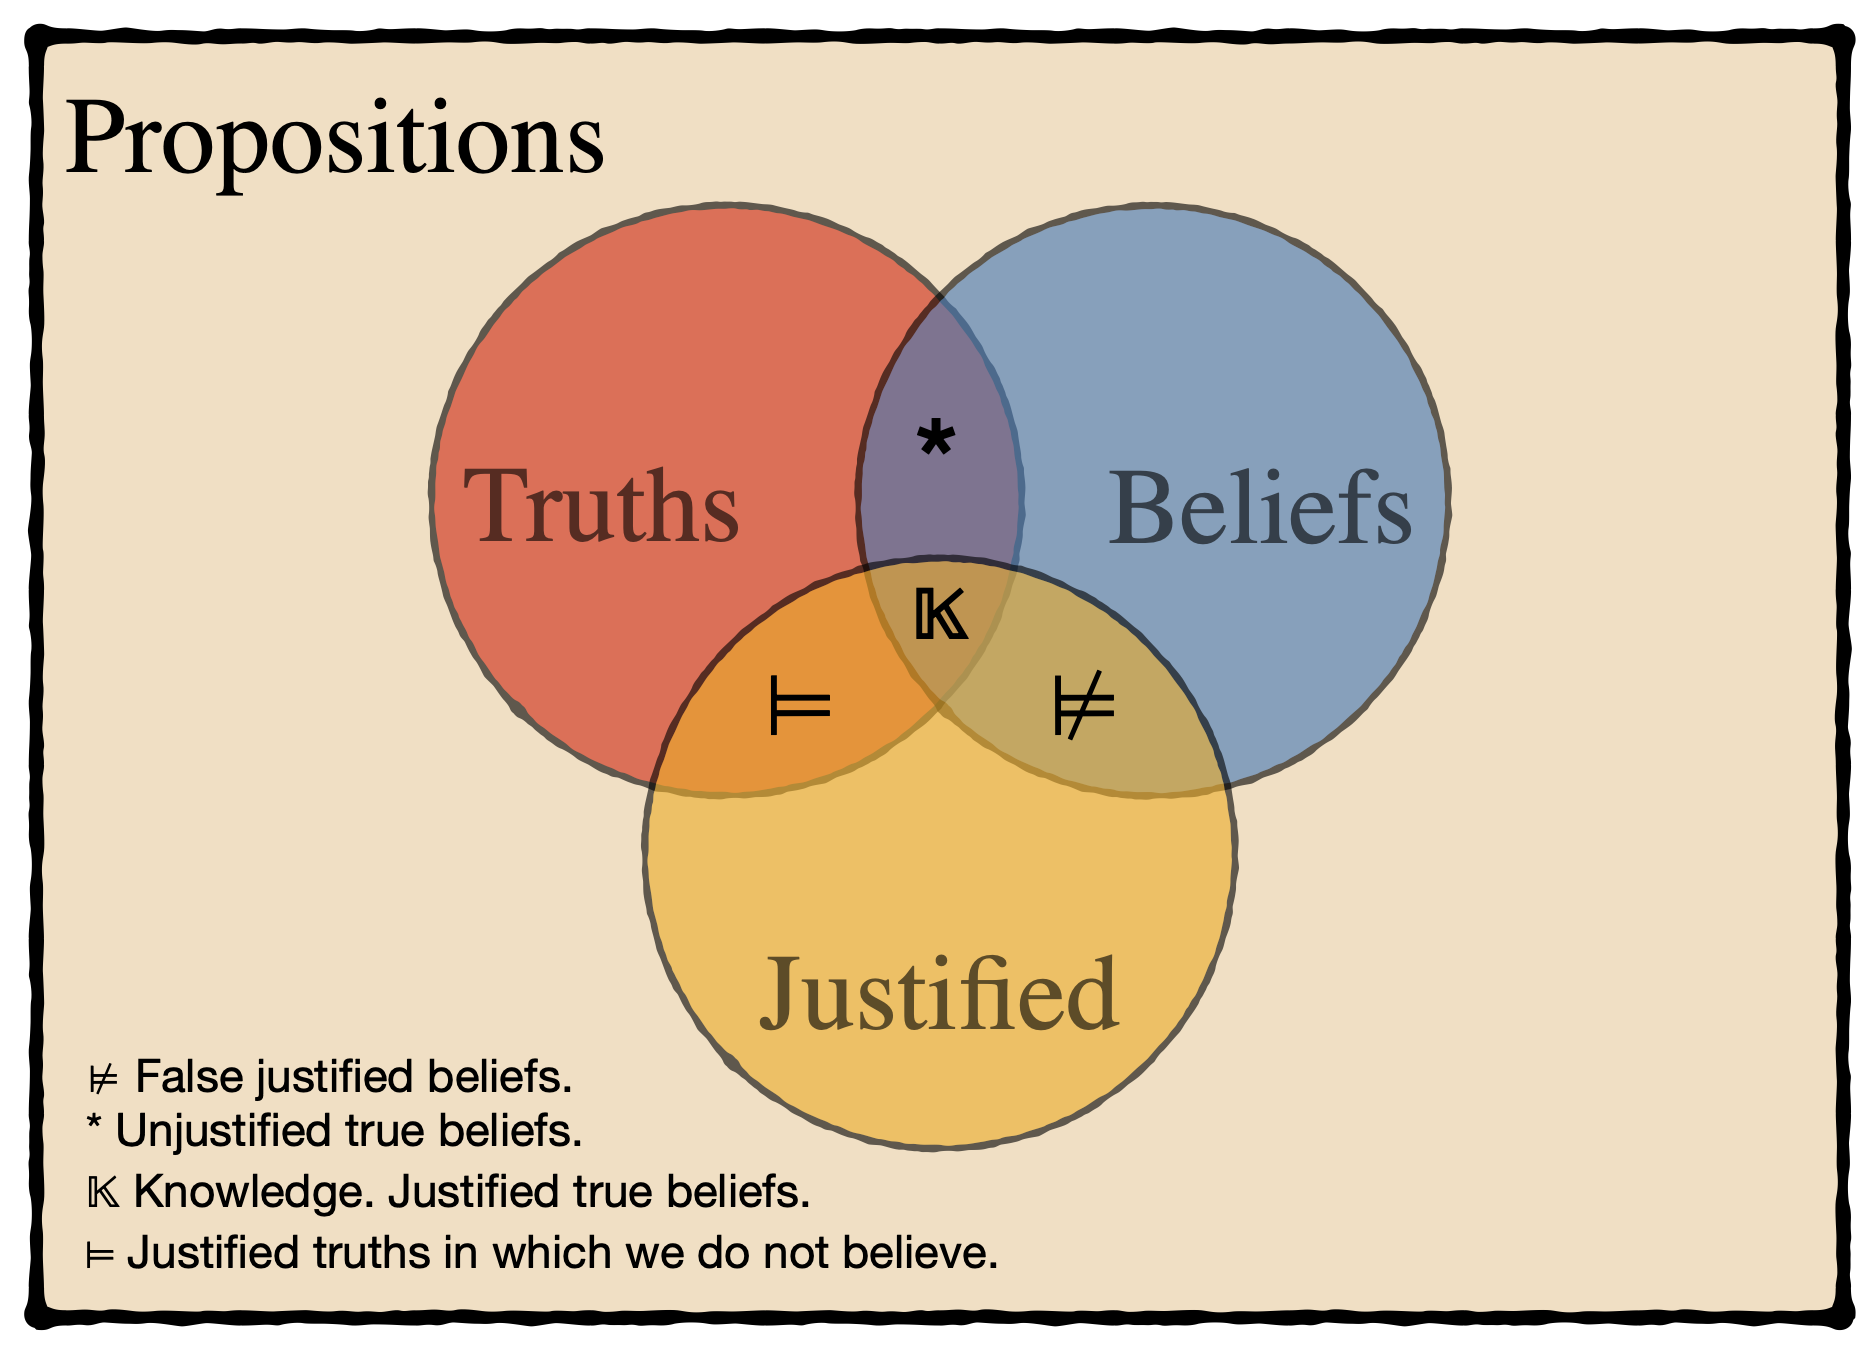
\includegraphics[width=1\linewidth]{Figures/knowledge} 

}

\caption{A Venn diagram illustrating the classical theory of knowledge.}\label{fig:plato-knowledge}
\end{figure}

Definitions should not be accepted without reason, and instead, we should attend to the arguments that support such definitions. Certain definitions may have widespread popularity but that doesn't make them any more true. For example, a dolphin is a mammal even if many people consider it a fish. In the same way, tomatoes and cucumbers are fruits for botanists even if we daily sort them as vegetables. And sometimes, even the \href{https://eur-lex.europa.eu/LexUriServ/LexUriServ.do?uri=CELEX:32001L0113:En:HTML\#d1e32-72-1}{EU} and \href{https://www.nationalgeographic.com/culture/article/fruit-or-vegetable}{the Supreme Court of the United States of America} need to act to set certain market debates.

As another example, the first astronomers who lacked the telescope believed on the geocentric model because their observations did not suffice to reject it. These first astronomers had \textbf{false justified beliefs}. After the advent of the telescope in 1609, the geocentric model was rejected. But how do we know we are not in a similar situation that of the pre-telescope astronomers? Events as recent as the Michelson-Morley (see \ref{michelson-morley}) experiment, the expeditions of Sir Arthur S. Eddington or the predictions of Urbain Le Verrier (see \ref{neptune-vulcan}) have changed our conceptions of the universe and physics forcing scientists to re-formulate models and theories.

In the next chapter we will see how knowledge is obtained.

\hypertarget{data-information-and-knowledge}{%
\subsubsection{Data, information and knowledge}\label{data-information-and-knowledge}}

Nowadays, technology allows us to collect data into datasets, transform datasets into information and arrive at new knowledge. Such processes have always been crucial in science but computer science comes to question concepts such as data, information and knowledge. \citep{johansson2016philosophy}

By \textbf{knowledge}, we can understand three different things. First, knowledge of truths, e.g.~we know that the sun rises on the east. Such knowledge can be obtained by reading a book or listening to the radio.
The second category of knowledge consists of skills, such as riding a bike or speaking a foreign language. However, this knowledge requires more than language to be communicated. It requires practice.
Finally, the third category is the knowledge of objects, what Bertrand Russell called knowledge by acquaintance \citep{russell2001problems}. This knowledge is obtained through experience.

In common English, we can't distinguish between knowledge of truths and objects. However, languages such as German, French or Spanish make clear this distinction by using different verbs, Rusell proposed to use the word ``acquaintance''.

\begin{itemize}
\tightlist
\item
  German: wissen vs kennen.
\item
  French: savoir vs connaître.
\item
  Spanish: saber vs conocer.
\end{itemize}

Example from William James (1890) --- ``I am acquainted with many people and things, which I know very little about, except their presence in the places where I have met them. I know the colour blue when I see it, and the flavour of a pear when I taste it; {[}\ldots{]}''

What is the difference between data and information?

The following excerpt from \citep{johansson2016philosophy} may clarify this question:

\begin{quote}
But why call the input `information'? The reason seems to be that we can describe the input as being about something, often the state of the environment. It has content. Or rather, when we humans describe the input and the workings of the system we find it natural to talk as if the information-containing system consciously sent messages to us humans; we say that the systems obtain information, transmit information or store information about something, as if it were like a human mind. The core feature of this use of the word `information' is thus its aboutness, its intentionality.
\end{quote}

\begin{quote}
Finally data. It is common in computer science to say that information is data with meaning. This is ok as far as it goes, but what is `meaning'? And how do data acquire meaning? It seems that minimally it means that meaningful data becomes information when we have been able to formulate declarative sentences expressing the information that is obtained from a data set. Almost anything can be data. In order to obtain data from e.g.~a story, from light from distant stars, or from the result of an experiment, we need to divide the stream of sounds, lights, or states of detectors into distinct items. When using written text as data source one must divide the string of linguistic signs into distinct items, such as words or longer or shorter expressions. {[}\ldots{]} In short, in order to obtain a data set, we need to define a principle for dividing up something into distinct pieces. Hence from a conceptual point of view, discerning data and collecting a data set presupposes that we have a prior principle of making distinctions within a phenomenon. {[}\ldots{]} Sometimes we have lot of background knowledge from start.
\end{quote}

\begin{quote}
In short, a piece of knowledge is a piece of information for which the knower can provide good reasons.
\end{quote}

\hypertarget{what-is-philosophy-of-science}{%
\subsection{What is Philosophy of Science?}\label{what-is-philosophy-of-science}}

One of the tasks of philosophy of science is to question assumptions that scientists take for granted. For example, suppose a scientist conducts an experiment that yields a particular result. The scientist then repeats the experiment a couple of times more obtaining the same result. The scientist then stops repeating the experiment, convinced that repeating it under the same conditions will produce the same result. But \emph{why} does the scientist assume that future repetitions will provide the same outcome? How are we sure this is true?

Therefore, one of the main objectives of philosophy of science is to study the methods and methodologies of enquiry used in the sciences, understanding how techniques like experimentation, observation and theory building enable scientists to reveal new knowledge. Philosophy of science asks questions such as: What is knowledge? What is a scientifically acceptable observation? What makes an explanation scientific? What is a scientific theory?

Finally, the philosophy of science tackles a wide range of topics that would require its own master. Moreover, not all topics are directly related to the aims of this course and the scope of the master. For this reason, a brief summary of the topics left behind is included in § \ref{wont-fix}. Of course, the curriculum is subject to change in the future and the list might change too.

\hypertarget{sci-method}{%
\section{The scientific method}\label{sci-method}}

The scientific method is the main pillar of science. All science begins with \emph{observation}, as this is the \textbf{first step} of the scientific method. Moreover, such observation must be \emph{repeatable}, either actually or potentially. Once an observation has been made, the \textbf{second step} involves the definition of a \emph{problem}, or in other words, asking a question about the observation. However, such a question needs to be valuable scientifically, it must be \emph{relevant} and must be \emph{testable}. Questions need to be reformulated until they become testable. The \textbf{third step} may seem a rather unscientific procedure as it involves guessing what the answer to the question might be by postulating a \emph{hypothesis}. The \textbf{fourth step} will tell the scientist if the \emph{hypothesis} is correct through \emph{experimentation}, which tests the validity of a scientific guess. Notwithstanding, experiments do not guarantee a scientific conclusion. Experiment results represent \emph{evidence}, i.e.~the hypothesis in answer to the question is confirmed as correct or invalidated. Given the latter, a new hypothesis with new experiments might be needed. Finally, experimental evidence is key for the \textbf{fifth step} of the scientific method, the formulation of a \emph{theory}. A good theory has a \emph{predictive} value, usually predicting that something is \emph{likely} to happen with a certain degree of probability \citep{pos-nidditch}.

\hypertarget{methodology}{%
\section{Methodology}\label{methodology}}

A method is a particular tool to reach a particular goal (e.g.~statistical test). Methodology is the systematic assessment and justification of method choice. Scientists often need to choose between alternative methods in order to reach a particular scientific goal. But specifying a goal does not directly determine what method to choose. We need to consider the reasons why some method is better than another for a particular goal. This process could require a better definition of the initial goal or learning more about the context and domain where the methods will be applied. Methodology must be distinguished from describing methods, which usually concerns the design and implementation of particular research approaches and focus on the technical aspects (e.g.~how to program simulations or set up instruments).

For example, a laboratory experiment can be advantageous because the test conditions can be controlled but laboratory experiments might not be realistic enough for certain tests. On the other hand, a field experiment provides more realistic test conditions but is difficult to control all variables.

Similar considerations may be necessary for other seemingly trivial questions such as model choice or data visualization. Should we use a significance test or a Bayesian approach? Should we present our results using a bar chart or a violin plot? Should we use a structural model or a quantum model? Methodology asks questions such as: What methods are available to reach a particular goal? What reasons speak for or against the alternatives? How should be weight the reasons to form a final decision?

How do we decide between alternative methods? Is there a way to determine what is rational to choose?
Traditionally there are three ways to choose between alternative methods.

\textbf{By convention,} The methods are chosen because you have been taught to, or because is an established convention between your peers. Conventionalisms create long-term issues when methods become dominant in a field. A good example is the use of p-value in hypothesis significance testing. Similarly, accuracy and precision metrics in Machine Learning can be considered conventionalism. More problems arise when different disciplines have different conventions, hindering inter-disciplinary work.

\textbf{Outcome-oriented.} While choosing the method that yields the best results may seem well-intended and appropriate, this certainly sounds very vague too. The intention is to find a method that serves some purpose best, but this purpose is sometimes not sufficiently clear. Science frequently involves long-term projects where the final material outcome is uncertain or unknown. For example, the International Space Station or the Large Hadron Collider. This methodology raises the question of how to measure the outcome. For instance, is speed the best way to assess which car is best? Should we focus on fuel autonomy or pollution instead? What about combining all of them?

\textbf{Reason-based.} Choosing the method based on the overall best reasons seems the best option, particularly when the reasons include considerations that justify choosing a method over others for a given scientific goal (e.g.~prediction). But sometimes there are methods that despite providing more valuable results could be unethical and/or illegal. For example, randomized control trials (RCT) are often employed to test the effectiveness of a new drug. Participants are divided \emph{at random} into two groups (treatment and control), eliminating the effect of confounding factors on the outcome of interest. However, RCTs are not always feasible, for either practical or ethical reasons. For instance, it won't be ethical to assign people to smoke for decades in order to study if cigarette smoking causes cancer. These other aspects need to be weighted together with the scientific reasons during method choice.

See \ref{smoke-debate} for an example of how reason-based methods are not always easy to implement while at the same time, outcome-oriented methods led the mainstream of an important debate.

\newpage

\hypertarget{examples}{%
\section{Examples}\label{examples}}

\hypertarget{neptune-vulcan}{%
\subsection{Neptune and Vulcan}\label{neptune-vulcan}}

Newton's gravitational theory predicted the paths the planets should follow as they orbit the sun. Most of these were confirmed by observation, but the orbit of Uranus differed from Newton's predictions. In 1846 John Adams in England and Urbain Le Verrier in France solved the mystery. Both of them suggested that another planet, yet undiscovered, was the cause of an additional gravitational force exerted on Uranus. These scientists calculated the mass and position that this planet would need to have to explain Uranus' orbit. The planet Neptune was indeed found close to the location predicted by Adams and Le Verrier.

So, instead of rejecting Newton's theory right away (see \ref{falsification}), these scientists stuck to it and tried to find another missing factor that could explain the difference. When the motion of Uranus was found not to match the predictions of Newton's laws, the theory ``There are seven planets in the solar system'' was rejected, and not Newton's laws themselves.

However, Le Verrier also found irregularities in the motion of the planet Mercury and tried to explain them as resulting from the gravitational pull of an, again, yet undetected planet Vulcan. This hypothetical planet would have to be a very dense and small object between the sun and Mercury. In this case, no planet was found between Mercury and the sun. A satisfactory explanation was provided much later by the general theory of relativity, which justified irregularities through a new system of laws. In this case, the hypothesis or theory had to be reformulated or replaced by new one.

Below you can find a \href{https://www.youtube.com/watch?v=j3mhkYbznBk\&t=1830s}{clip from lecture ``The Law of Gravitation''}, from the Messenger Lectures given by the renowned American theoretical physicist Richard Phillips Feynman.

\hypertarget{michelson-morley}{%
\subsection{The most famous ``failed'' experiment}\label{michelson-morley}}

The Michelson-Morley experiment (1887) was designed to detect the motion of the Earth through the luminiferous aether. XIX century physicists used aether to explain how light could be transmitted through empty space between the Sun and the Earth. The result of this experiment is considered to be the first strong evidence against the then-prevalent aether theory, and the beginning of a new line of research that eventually led to special relativity, which rules out a stationary aether.

To the ancients, the concept of a void universe was impossible. Aristotle arrived at the hypothesis of the aether to explain the cosmos and several natural phenomena such as the movement of the planets. By the XIX century, the aether became more than a philosophical need. Whenever there is a wave, something must be waving. But what waves when light waves travel from the Sun? For XIX physicists, the aether was the medium through which light waves from the Sun would propagate.

Michelson and Morley attempted to detect the absolute motion of Earth through space. For that, they set an experiment in which a beam of light was sent through a half-silvered mirror used to split the light beam into two beams travelling at right angles to one another. The beams were then reflected back to the half-silvered mirror by two respective mirrors and recombined into a single beam. The experiment can be seen as a race between two light beams. If the beams arrive in a tie, the result is a bright spot at the centre of the interference pattern, otherwise, a destructive interference would make the centre of the image dark. The hypothesis foretold that a tie was not possible since the two beams were racing on a moving track. It was assumed that the Earth was moving through the aether and therefore the beam should trace different paths with respect to the aether.

The extent to which the negative result of the Michelson--Morley experiment influenced Einstein is disputed. However, the null result helped the notion of the constancy of the speed of light gain acceptance in the physics community. This example shows the impact a well-designed experiment can have.

For a longer and deeper explanation of the experiment, its historical context and consequences, watch \href{https://www.youtube.com/watch?v=Ip_jdcA8fcw}{episode 41 from The Mechanical Universe}. The timeline of luminiferous aether can be found \href{https://en.wikipedia.org/wiki/Timeline_of_luminiferous_aether}{at the Wikipedia}.

\hypertarget{eddington-expeditions}{%
\subsection{Eddington expeditions}\label{eddington-expeditions}}

\begin{wrapfigure}{R}{.25\textwidth}  
 \begin{center}
    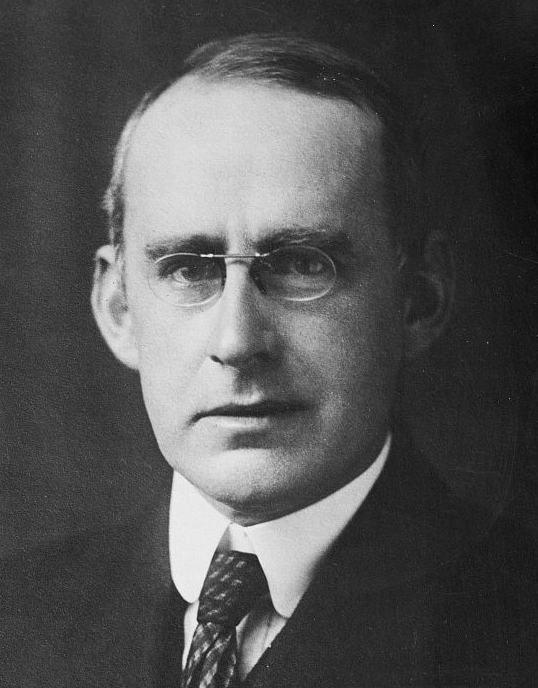
\includegraphics[width=.22\textwidth]{Figures/Arthur_Stanley_Eddington.jpg}  
  \captionsetup{labelformat=empty}
  \caption{Sir Arthur Stanley Eddington (1882–1944).} 
\end{center}
\end{wrapfigure}
\addtocounter{figure}{-1}

The following example also relates to falsification (see \ref{falsification}) which is taught in the next Chapter. However, this is also a good example of how a good theory should make definite predictions such as those from Einstein's theory of general relativity.

Figure \ref{fig:eddington-eclipse} shows the positions of different stars during the eclipse. Such stars are not normally visible in the daytime due to the brightness of the Sun but become visible during the moment when the Moon fully covers the solar disc. A difference in the observed position of the stars during the eclipse, compared to their normal position at night, indicates that the light from these stars had bent as it passed close to the Sun.



\begin{quote}
Einstein's theory made a clear prediction: light rays from distant stars would be deflected by the gravitational field of the sun. Normally this effect would be impossible to observe --- except during a solar eclipse. In 1919 the English astrophysicist Sir Arthur Eddington organized two expeditions to observe the solar eclipse of that year, one to Brazil and one to the island of Principe off the Atlantic coast of Africa, with the aim of testing Einstein's prediction. The expeditions found that starlight was indeed deflected by the sun, by almost exactly the amount Einstein had predicted. Popper was very impressed by this. Einstein's theory had made a definite, precise prediction, which was confirmed by observations. Had it turned out that starlight was not deflected by the sun, this would have shown that Einstein was wrong. So Einstein's theory satisfies the criterion of falsifiability. --- \citep{okasha-pos}
\end{quote}

\begin{figure}

{\centering 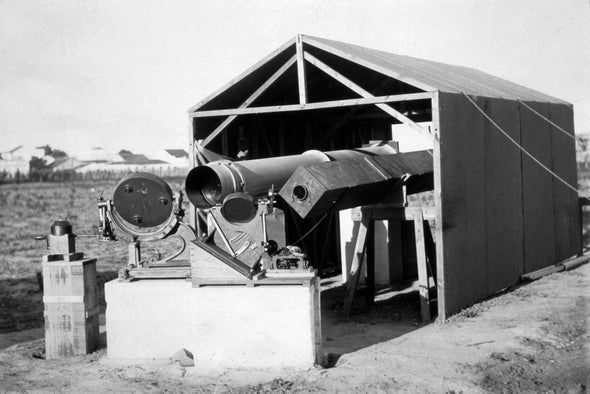
\includegraphics[width=0.5\linewidth]{Figures/eddington-instruments} 

}

\caption{Instruments used in the 1919 observations to test Einstein's predictions about warped spacetime. Credit: Getty Images}\label{fig:eddington-instruments}
\end{figure}

\begin{quote}
Einstein published his general theory of relativity in 1915. The total solar eclipse of 1919 offered the perfect opportunity to test it experimentally, by exploring whether --- and how --- the immense gravity of the Sun bends and distorts incoming light from more distant stars, as predicted by Einstein's theory. For a brief moment during the eclipse, the Moon would block the Sun's light in the sky and make visible some of the stars that lie close to the line of sight of the Sun, not normally visible during the daytime. By measuring the positions of these stars during the eclipse and comparing them to their positions at night, when the sun is not in the field of view, it would be possible to determine whether their light rays bends while passing close to the Sun. --- European Southern Observatory
\end{quote}

\begin{figure}

{\centering 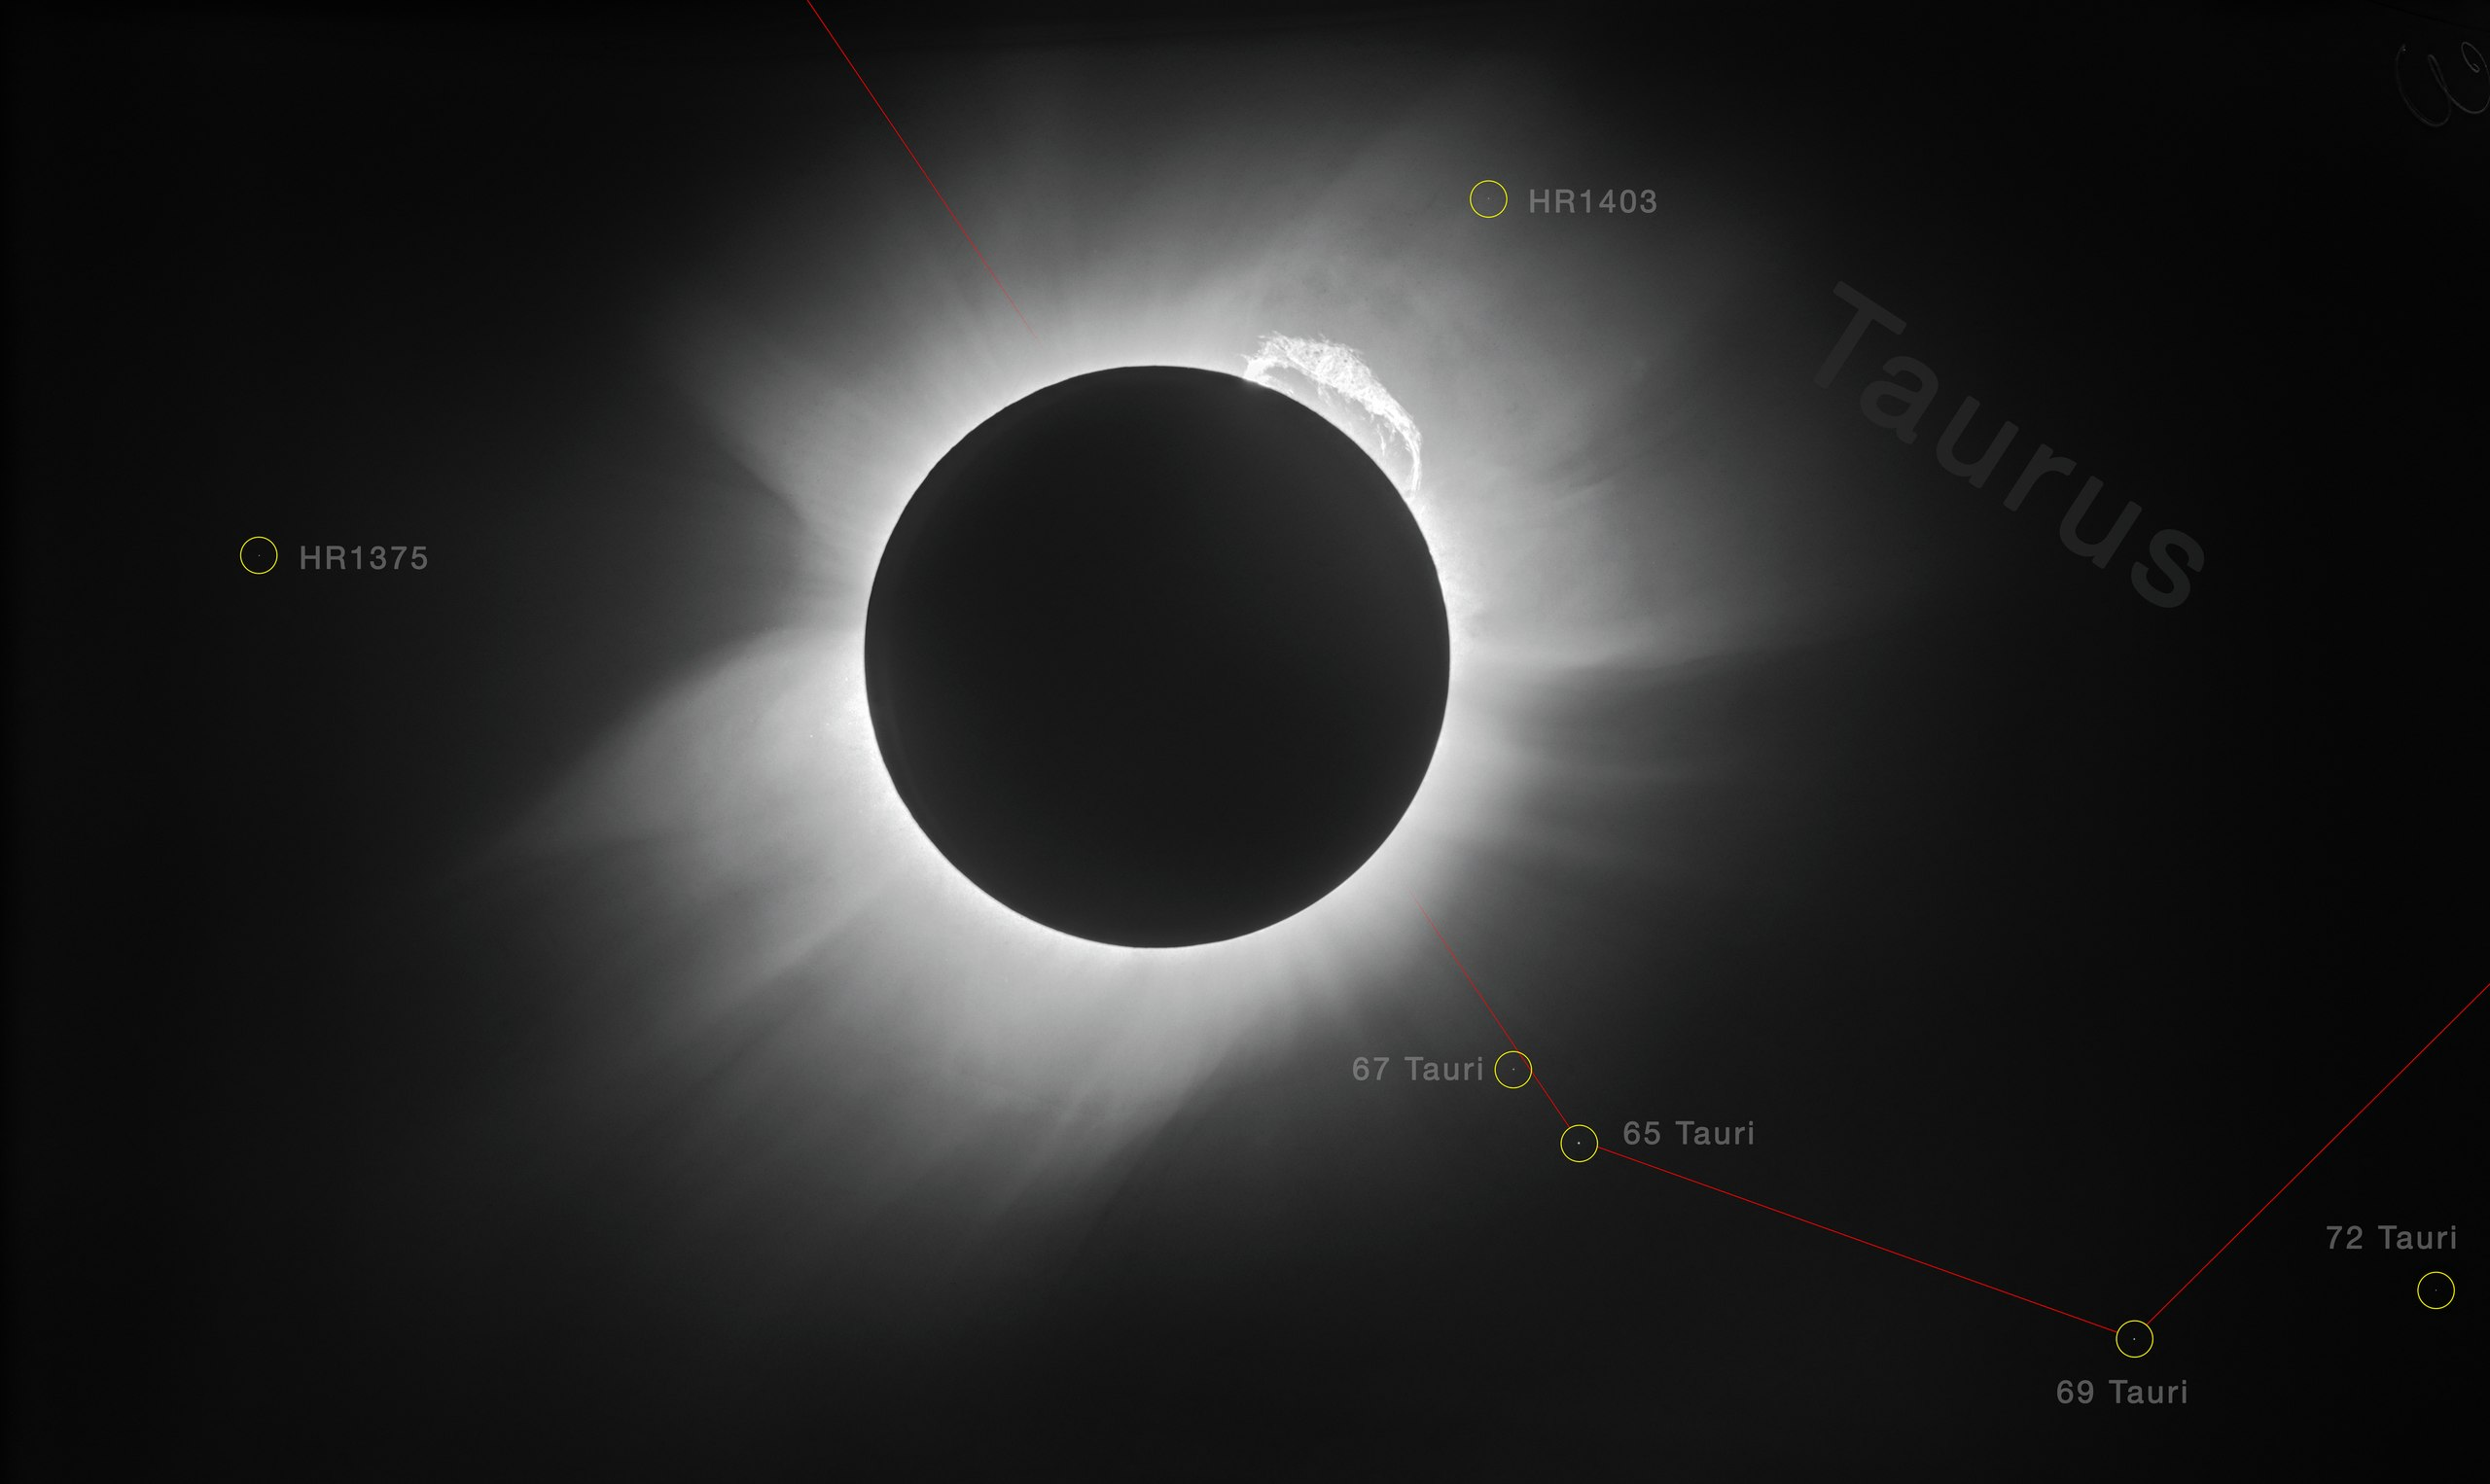
\includegraphics[width=1\linewidth]{Figures/solar_eclipse} 

}

\caption{Eddington and Crommelin imaged the eclipse using the technology of the time: photographic plates made of glass. Sadly, the original plates from the 1919 expedition have been lost --- but, luckily, copies of one of the plates were made and sent to observatories around the world to allow scientists everywhere to see the evidence in support of relativity with their own eyes. Source: \href{https://www.eso.org/public/images/potw1926a/}{European Southern Observatory}.}\label{fig:eddington-eclipse}
\end{figure}

\begin{quote}
One of the interesting facts from Stanley's account is that Einstein had made a stab at calculating the bending of light back in 1911, before he had formulated the full general theory of relativity. His result was precisely the same as the Newtonian value. I was left wondering what would have happened to his reputation if measurements had been taken then. Would they have been a setback? Or would they just have driven him harder to produce the full theory, with its crucial factor of two? --- \citep{coles2019einstein}
\end{quote}

\hypertarget{smoke-debate}{%
\subsection{The smoke debate}\label{smoke-debate}}

In the mid-1700s, James Lind discovered that citrus fruits prevent scurvy, while in the mid-1800s, John Snow figured out that water contaminated with faecal matter caused cholera. These two examples share a common fortunate one-to-one relation between cause and effect. Deficiency of vitamin C is necessary to produce scurvy. Similarly, cholera bacillus is the only cause of cholera.

However, during the late 1950s and early 1960s, whether or not smoking caused lung cancer was not clear. The subject of the debate wasn't tobacco or cancer but rather the word \emph{caused} as one of the most important arguments against the smoking-cancer hypothesis was the possible existence of confounding factors that may cause lung cancer and nicotine dependency. Many smokers live long lives without getting lung cancer while others develop cancer without ever smoking. Plotting the rates of lung cancer and tobacco consumption makes the connection impossible to miss (See Figure \ref{fig:smoke-ts}). However, time-series data are poor evidence for causality. Researchers already knew about RCT though its use was unethical in this case.



\begin{figure}

{\centering 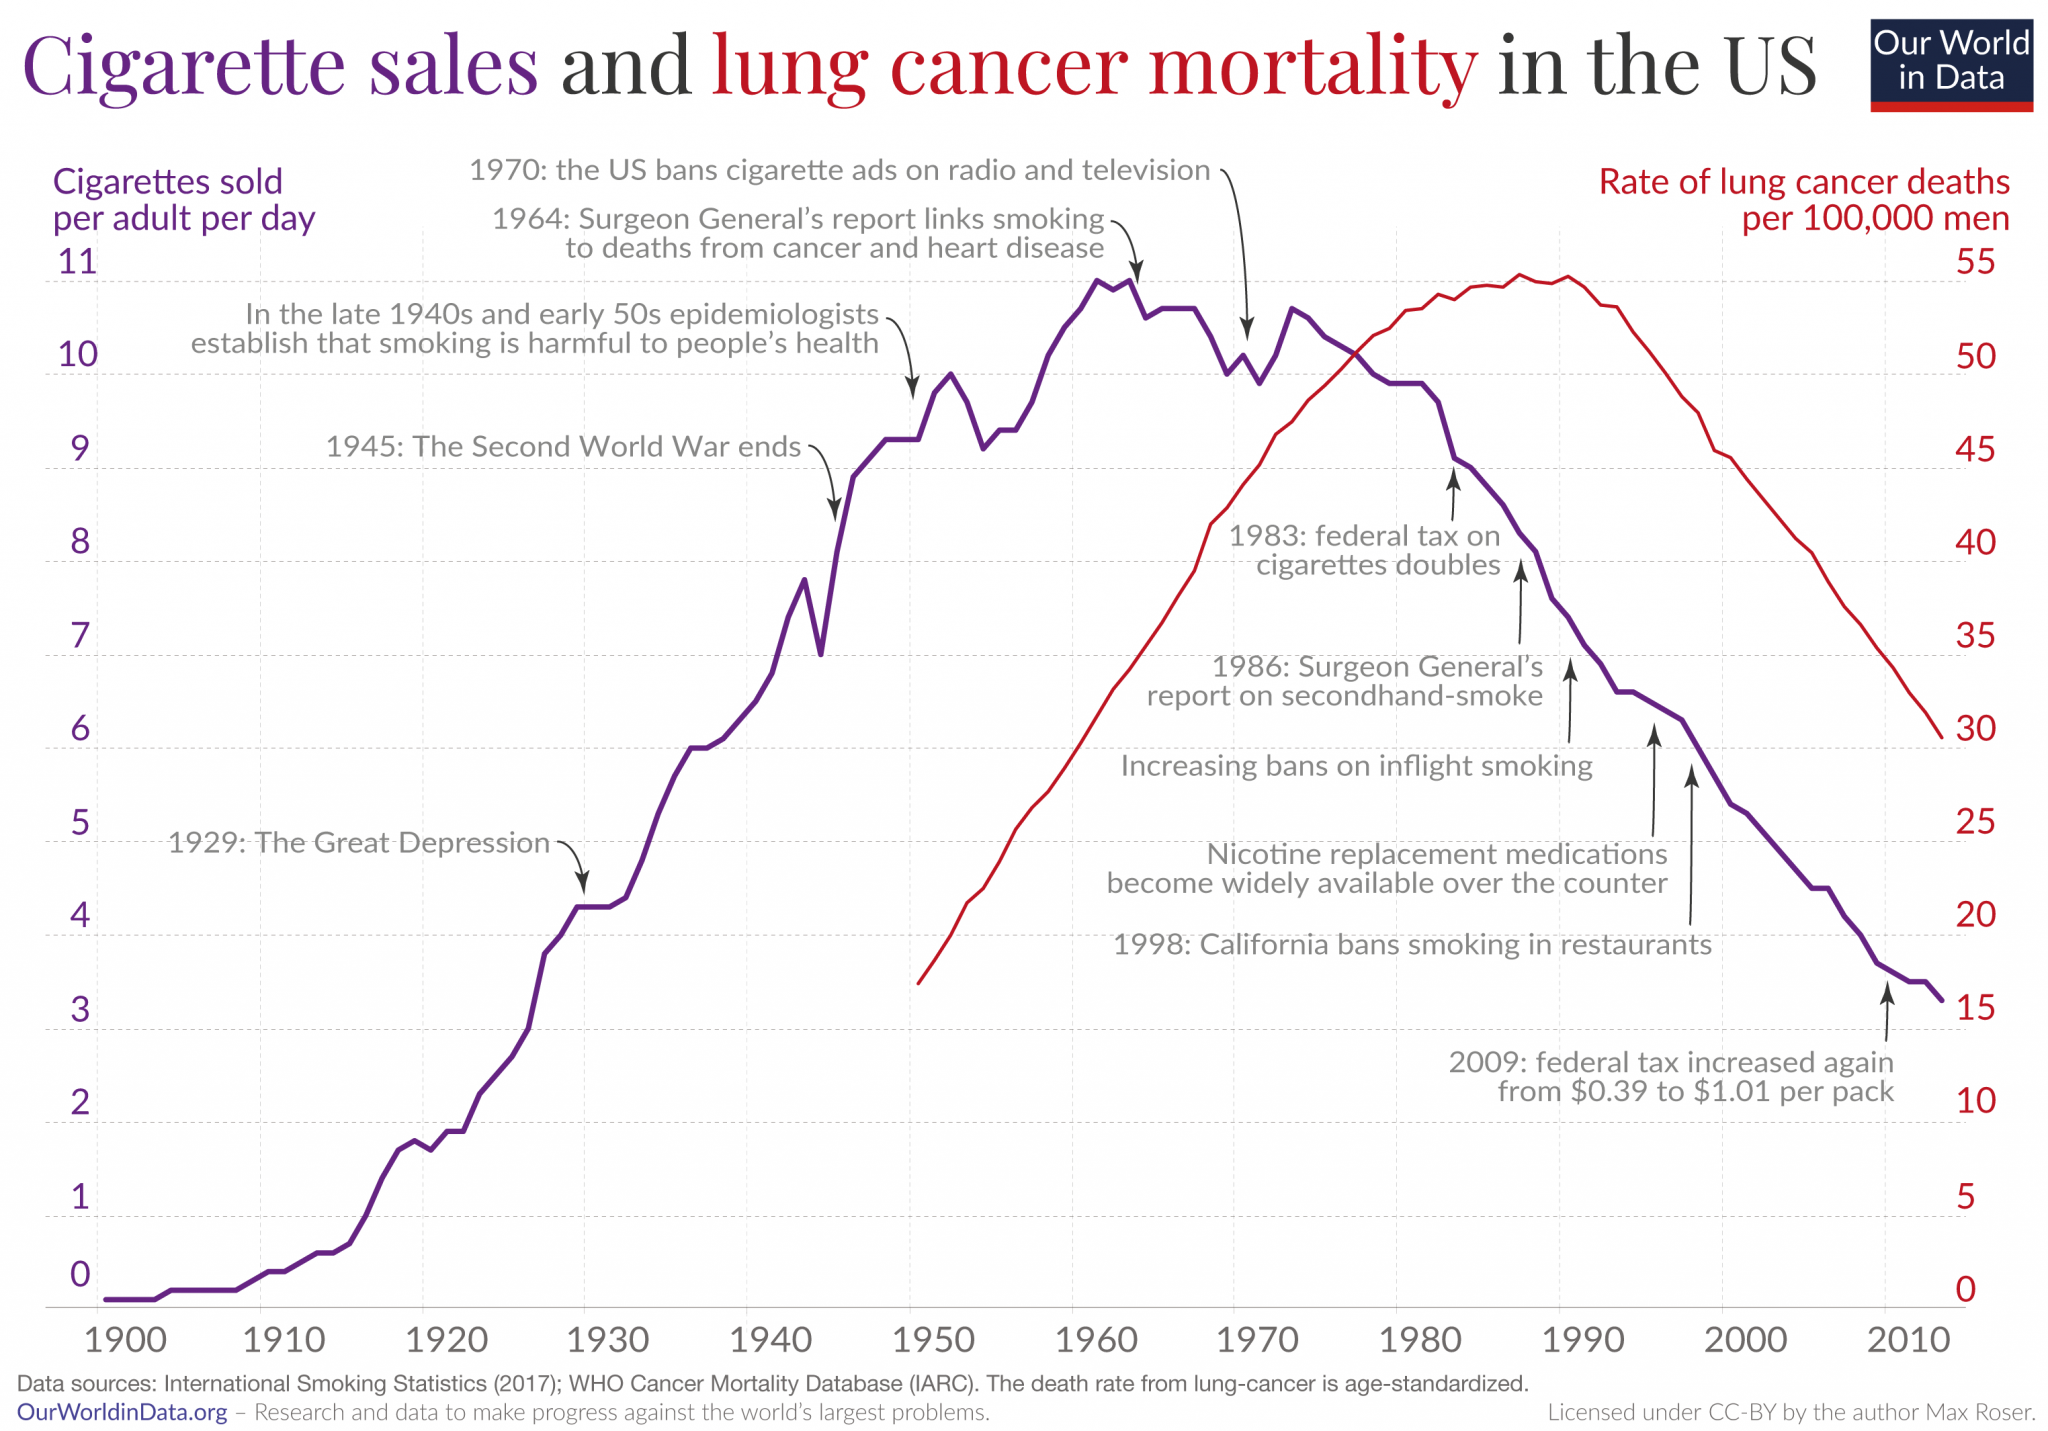
\includegraphics[width=0.75\linewidth]{Figures/Smoking-and-lung-cancer-mortality-US-only} 

}

\caption{Source: \href{https://ourworldindata.org/smoking-big-problem-in-brief}{Our World in Data}.}\label{fig:smoke-ts}
\end{figure}

Austin B. Hill proposed to compare patients already diagnosed with cancer to a control group of healthy volunteers. The results showed that all but two of the 649 lung cancer patients had been smokers. This type of study is today called a case-control study because it compares cases to controls. However, \textbf{this method has some drawbacks too}. First, the study is retrospective, meaning that participants known to have cancer are considered and researchers look back to understand why. Second, the probability logic is backwards, as the data tell us the probability that a cancer patient is a smoker instead of the probability that a smoker will get cancer. Moreover, case-control studies admit several possible sources of bias such as recall bias or selection bias. Hospitalised cancer patients were not a representative sample of the population, not even from the smoke population. Researchers were careful to call their results an ``association''. Later on, the study was replicated with similar results. Deniers such as R. A. Fischer were right to point out that repeating a biased study doesn't make it any better as is still biased.

We won't focus on how this story ends here but \textbf{is important to notice how methods chosen based on scientific reasons are sometimes tough to implement and often need to fight against outcome-oriented studies} such as those sponsored by leading tobacco companies.

In the end, many subsequent studies settled the smoking-cancer debate. We will come back to this example in upcoming sections of the course. If you can't wait, read Chapter 5 from the Book of Why, by Judea Pearl and Dana Mackenzie \citep{book-of-why}.

\hypertarget{kekuluxe9s-dream}{%
\subsection{Kekulé's dream}\label{kekuluxe9s-dream}}

The third step of the scientific method (see § \ref{sci-method}) requires guessing an answer (or hypothesis) to a previously determined question. There is no clear method to arrive at a hypothesis. Experience, historical context, and previously failed hypothesis condition how a hypothesis is conceived. But sometimes hypotheses can be reached in the most unlikely and unconventional of ways. It makes no difference as long as the hypothesis is then scientifically tested before its acceptance. One of the most famous examples is the structural model of the benzene molecule. In 1865 the chemist August Kekulé hit on the hypothesis of the structure after dreaming of a snake trying to bite its tail (See Figure \ref{fig:ouroboros}).



\begin{figure}

{\centering 
\includegraphics[width=0.25\linewidth]{Figures/Ouroboros-benzene} 

}

\caption{Source and credits to: Haltopub, from \href{https://en.wikipedia.org/wiki/File:Ouroboros-benzene.svg}{Wikimedia}.}\label{fig:ouroboros}
\end{figure}

\hypertarget{scientific-inference}{%
\chapter{Scientific Inference}\label{scientific-inference}}

\hypertarget{overview}{%
\section{Overview}\label{overview}}

Humans have a natural ability to conjecture and spot relationships about the world, \emph{jumping} from hypotheses to conclusions. The scientific attitude is to keep such \emph{jumps} under control and use a well defined procedure to arrive to a conclusion from an hypothesis. In this chapter we will examine in detail those procedures.

\begin{quote}
But our sun is only one of a billion-trillion stars within the observable universe. And those countless suns all obey natural laws some of which are already known to us. How did we discover that there are such laws? If we lived on a planet where nothing ever changed, there wouldn't be much to do, there'd be nothing to figure out. There'd be no impetus for science. And if we lived in an unpredictable world where things changed in random or very complex ways, we wouldn't be able to figure things out. And again, there'd be no such thing as science. But we live in an in between universe where things change alright, but according to patterns, rules, or as we call them, laws of nature. If I throw a stick up in the air, it always falls down. If the sun sets in the west, it always rises again the next morning in the east. And so it's possible to figure things out. We can do science. And with it we can improve our lives. --- Carl Sagan
\end{quote}

\hypertarget{types-of-inferences}{%
\section{Types of inferences}\label{types-of-inferences}}

Most scientific conclusions are uncanny at first glance and difficult to believe without more information and proper explanations about them (e.g.~expansion of the universe, electromagnetism, etc.). How do scientists reach such unlikely conclusions? An inference is the act of reaching a conclusion from known facts but there are multiple types as we will see below.

\hypertarget{deduction}{%
\subsection{Deduction and Induction}\label{deduction}}

A good argument is one whose conclusions follow from its premises. But how do we tell if the conclusion is a consequence of its premises? Is often assumed that as long as the premises are valid, the conclusions will be valid too. This does not imply that the conclusion is also true. The premises might not be true, but if they are true, then the conclusion will also be true. However, is the truth of the premises always \emph{necessarily sufficient} for the truth of the conclusions? Logicians distinguish between deductive and inductive inference. \citep{sep-abduction}

Below there is an example of a deductive inference with two premises followed by a conclusion.

\begin{verbatim}
All Frenchmen like cheese
Loubin is a Frenchman
------------------------------
Therefore, Loubin likes cheese
\end{verbatim}

\begin{verbatim}
All As are Bs
a is an A
--------------------
Therefore, a is a B
\end{verbatim}

We call an inference \emph{deductive} whenever the conclusion \emph{necessarily} follows from the premises. \textbf{The truth of the premises \emph{guarantees} the truth of the conclusion.} Or in other words, what is inferred is \emph{necessarily} true if the premises from which it is inferred are true. We call this type of inferences \emph{explicative}.

Not all inferences are deductive. For example:

\begin{verbatim}
The first five eggs in the box were good.
All the eggs have the same best-before date stamped on them.
------------------------------------------------------------
Therefore, the next egg will be good too.
\end{verbatim}

In this case, the premises do not entail the conclusion. Even if the previous eggs were good, it is possible that the next egg will be rotten. In this case, is logically possible for the premises to be true and yet the conclusion false. We call this type of inferences \emph{inductive}. Contrary to deduction, where the truth of the premises guarantees the truth of the conclusion, \textbf{inductive inferences are \emph{ampliative} --- since whose conclusions go beyond what is contained in their premises ---} and their conclusions could be totally wrong even if infinitely many examples confirm them. \citep{bergadano1991problem}

In these regards, deduction seems safer than induction. Whenever we reason deductively we can be sure that given true premises we will reach true conclusions. On the other hand, \textbf{inductive reasoning can take us from true premises to a false conclusion}. Notwithstanding, we rely on inductive reasoning every day. For instance, every day we turn on our computers and we are confident they will not explode in our faces. \citep{okasha-pos} But why? Simply because we do it every morning and it has never exploded up to now.

We are sure that the sun will rise tomorrow, and if we are asked why we believe so, we will naturally answer ``Because it always does''. We believe that it will rise in the future because it has risen in the past. Of course, when we are challenged to answer what \emph{justifies} our belief we can refer to the laws of motion and nature. But will the laws of motion remain the same tomorrow? \citep{russell2001problems}

\hypertarget{modus}{%
\subsection{Modus ponens and Modus tollens}\label{modus}}

\begin{notebox}

\begin{center}
\textbf{Course Note:}

\end{center}

The following content relates to deduction and is usually taught in high school philosophy courses as part of propositional calculus. It will help getting a better understanding of the deductive inference rules. If this is already clear to you, feel free to jump to the problem(s) of induction \ref{problem-induction}.

\end{notebox}

There are two rules of inference in deductive reasoning. Deduction constitutes top-down logic because particular conclusions are drawn from general premises. Whereas in bottom-up logic the conclusion is reached by generalizing from specific cases.

\begin{itemize}
\tightlist
\item
  Modus ponens: \texttt{P\ implies\ Q.\ P\ is\ true.\ Therefore\ Q\ must\ also\ be\ true.}
\item
  Modus tollens: \texttt{If\ P,\ then\ Q.\ Not\ Q.\ Therefore,\ not\ P.}
\end{itemize}

The form of a \textbf{modus ponens} argument looks like a syllogism consisting of two premises and a conclusion. The first premise is a conditional if-then claim (e.g.~\texttt{P\ implies\ Q}). The second premise is an assertion that \(P\) (the antecedent of the first premise) is indeed true. From these two premises, it can be concluded that \(Q\), (the consequent of the first premise) must be true as well.

\begin{verbatim}
If P, then Q.
P.
--------------
Therefore, Q.
\end{verbatim}

The next example fits the form of \emph{modus ponens}.

\begin{verbatim}
If today rains, John will take the umbrella.
Today is raining.
------------------
Therefore, John will take the umbrella.
\end{verbatim}

The argument is valid but it doesn't matter if the statements in the argument are actually true. An argument can be valid but nonetheless unsound if their premises are false. \emph{Modus ponens} rule can be written as \(P \rightarrow Q, P \vdash Q\). In logic, an argument is sound if it is both valid in form and its premises are true.

On the other hand, the form of a \textbf{modus tollens} argument also consists of two premises and a conclusion. The first premise is a conditional if-then claim (e.g.~\texttt{P\ implies\ Q}). The second premise is an assertion that \(Q\) (the consequent of the conditional claim) is not the case. From these two premises, it can be concluded that \(P\) is also not the case. \emph{Modus tollens} rule can be written as \(P \rightarrow Q, \lnot Q \vdash \lnot P\).

\begin{verbatim}
If P, then Q.
Not Q.
-----------------
Therefore, not P.
\end{verbatim}

Modus tollens is specially important in falsification (see \ref{falsification}). For instance, we take our hypothesis H to test and assume that is true. If \(H\) is true, then consequent \(C\) is true. We make an observation and see that \(C\) is false. Therefore, we conclude that H is false.

\begin{verbatim}
If H, then C.
C is false.
-----------------
Therefore, H is false.
\end{verbatim}

\begin{center}\rule{0.5\linewidth}{0.5pt}\end{center}

Other forms of arguments are apparently \textbf{similar but invalid forms}.

\textbf{Affirming the consequent}. This formal fallacy consists of taking a true conditional statement \(P \rightarrow Q\) and invalidly inferring its converse \(Q \rightarrow P\). For example, the statement ``if the light is broken, the room would be dark'' does not justify inferring the converse ``the room is dark, therefore the lamp is broken''. This situations may arise when a consequent has more than one possible antecedent.

\textbf{Denying the antecedent}. This fallacy is committed by reasoning in the form: \texttt{If\ P,\ then\ Q.\ Therefore,\ if\ not\ P,\ then\ not\ Q}. This kind of arguments can seem valid at first glance. Consider this famous example from Alan Turing:

\begin{quote}
If each man had a definite set of rules of conduct by which he regulated his life he would be no better than a machine. But there are no such rules, so men cannot be machines. --- Alan Turing
\end{quote}

Men could still be machines that do not follow a definite set of rules.

Another trivial example of this second fallacy.

\begin{verbatim}
If you are a bus driver, then you have a job.
You are not a bus driver.
---------------------------
Therefore, you have no job.
\end{verbatim}

\hypertarget{problem-induction}{%
\section{The problem(s) of induction}\label{problem-induction}}

\textbf{Do scientists use induction?} Pretty much all the time. Whenever scientists move from limited data to general conclusions scientists reason inductively. \textbf{In inductively valid arguments, the (joint) truth of the premises is very likely (but not necessarily) sufficient for the truth of the conclusion.} For instance, a newspaper may run the headline ``scientists find experimental proof that transgenic maize is safe to eat''. This means scientists tested transgenic maize on a large number of people without finding any issues. Does this \emph{strictly prove} that transgenic maize is safe? Is this prove as strong as the proof of the Pythagoras' theorem? Going from ``the transgenic maize didn't harm any of the people on whom it was tested'' to ``the transgenic maize will not harm anyone'' is an inductive inference, not deductive.

\begin{tipbox}

\textbf{Writing Note:}

Suppose the following inductive inference \(I\): If the probability of observing \(R\), given that \(H\) is true, is smaller than a significance level of 0.05, then reject \(H\). Is important to distinguish between the two following things:

\begin{itemize}
\tightlist
\item
  Justification \emph{with} an inference rule: Justifying the conclusion by pointing to the premise and the inference rule. Inference rules justify conclusions.
\item
  Justification \emph{of} an inference rule: What makes \(I\) a good inductive inference? Why not choosing other parameters? The choice of a particular inference rule must be justified.
\end{itemize}

\end{tipbox}

\hypertarget{david-humes-problem-of-induction}{%
\subsection{David Hume's Problem of Induction}\label{david-humes-problem-of-induction}}

\begin{wrapfigure}{R}{.33\textwidth}  
 \begin{center}
    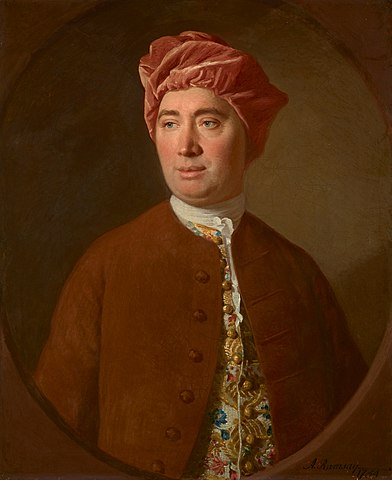
\includegraphics[width=.30\textwidth]{Figures/David_Hume.jpg}  
  \captionsetup{labelformat=empty}
  \caption{Portrait of David Hume by Allan Ramsay.} 
\end{center}
\end{wrapfigure}
\addtocounter{figure}{-1}

We use induction to justify our statements but how do we justify induction itself? How would you convince someone else that induction is a good inference method? The Scottish philosopher David Hume (1711-76) argued that the use of induction cannot be rationally justified at all. In 1739, still under the shadow of the bubonic plague in Europe, David Hume publishes \emph{A Treatise of Human Nature}, presumably without knowing that his work would not only continue to be debated more than 200 years later, but also still remarkably relevant in the technological advances of our time. In \emph{the problem of induction} Hume argues that we cannot make a causal inference just by \emph{a priori} means, and poses the question of how we can conclude from the observed to the unobserved.

Hume admitted that we use induction all the time in everyday life and science but insisted that this is just a matter of brute animal habit. What does he mean by that? Bertrand Russell (1872-1970) gives us a good example on this. He argues that the inductive association is also present in animals.

\begin{quote}
``And this kind of association is not confined to men; in animals also it is very strong. A horse which has been often driven along a certain road resists the attempt to drive him in a different direction. Domestic animals expect food when they see the person who usually feeds them. We know that all these rather crude expectations of uniformity are liable to be misleading. The man who has fed the chicken every day throughout its life at last wrings its neck instead, showing that more refined views as to the uniformity of nature would have been useful to the chicken. {[}\ldots{]} The mere fact that something has happened a certain number of times causes animals and men to expect that it will happen again. Thus our instincts certainly cause us to believe that the sun will rise to-morrow, but we may be in no better a position than the chicken which unexpectedly has its neck wrung.'' --- \citep{russell2001problems}
\end{quote}

Hume arrived to this conclusion by noting that whenever we make inductive inferences we presuppose the \emph{uniformity of nature}. Remember the eggs box example in § \ref{deduction} ? Our reasoning depends on the assumption that objects that we have not examined yet will resemble those objects that we have already examined. Then, Hume argues that we cannot prove the truth of the uniformity assumption. Basically, from the mere act of being able to imagine a world where nature is not uniform but changes at random it follows that we cannot prove that the uniformity assumption is true. Also, if we try to argue for the uniformity assumption on empirical grounds, we end up reasoning in a circle.

The conclusion then is that our tendency to project past regularities into the future is not underpinned by reason. The problem of induction is to find a way to avoid this conclusion, despite Hume's argument \citep{sep-induction-problem}. \textbf{Hume's problem of induction is still an active area of research for philosophers}. There are many different ways to respond to Hume's argument, yet none is fully convincing. Peter Strawson (1950s) used the following analogy: justifying induction is like asking whether the law is itself legal. This is rather odd, since the law is the standard against which the legality of other things is judged. Others, like Karl Popper (1902-1994) argued that science is not in fact based on inductive inferences at all and presented a deductivist view of science. We will study this in detail in § \ref{falsification}.

\begin{tipbox}

\textbf{Note on uniformity of nature:}

Notice how Machine Learning (ML) models can be regarded as inductive machines performing inductive inferences based on previous observations. For the ML model to perform well on novel data, is often assumed that novel data will resemble past data.

Hume refers to this assumption as the Principle of Uniformity of Nature: \emph{``If reason determined us, it would proceed upon that principle, that instances, of which we have had no experience, must resemble those, of which we have had experience, and that the course of nature continues always uniformly the same.''}

And it continues: \emph{``Our foregoing method of reasoning will easily convince us, that there can be no demonstrative arguments to prove, that those instances, of which we have had no experience, resemble those, of which we have had experience. We can at least conceive a change in the course of nature; which sufficiently proves, that such a change is not absolutely impossible. To form a clear idea of any thing, is an undeniable argument for its possibility, and is alone a refutation of any pretended demonstration against it.''}

\citep{hume1739treatise} T. 1.3.6.4

\end{tipbox}

As scientists, Hume's problem of induction may leave a huge void in our heart. An empty feeling that science is indeed fallible and the sudden realisation of the impossibility of establishing the truth or falsity of scientific laws \citep{rosenberg2019philosophy}. But perhaps there is a way to fill such gap, and perhaps big part of the effort of science is put on filling this void with as much certainty as possible.

Hume's argument concerns specific inductive inferences such as \texttt{All\ observed\ instances\ of\ A\ have\ been\ B} and \texttt{The\ next\ instance\ of\ A\ will\ be\ B}. Hume's argument proceeds as follows:

\begin{itemize}
\tightlist
\item
  Every inference is either inductive or deductive.
\item
  To justify an inductive inference rule \(I\), this rule must be inferred from some premises.
\item
  Is not possible to infer the rule \(I\) deductively, because there are no necessary connection between past and future inferences.
\item
  Therefore, the rule \(I\) must be inferred inductively.
\item
  When inferring \(I\) inductively, we must invoke another inductive inference rule \(J\) to justify this induction. But then, how do we justify \(J\)? \ldots{} {[}\emph{infinite regress}{]}
\end{itemize}

Just because an inference rule has yield true conclusions in the past does not necessarily imply that it will do so in the future.
Consequently, Hume concludes that no inductive inference rule can be justified. But, does this mean all scientific inductive inferences are not justified?

\begin{tipbox}

\textbf{Note for data scientists!}

If we visualise the data as points in a plane; every set of finite points belongs to infinite functions or curves. The problem of induction, in this case, consists in establishing criteria that allow us to say that the finite series of data confirms only one of the functions, or less dramatically but just as problematic, that one is more confirmed than the others \citep{diez1997fundamentos}. (See the problem of underdetermination in §\ref{confirmation}).

\end{tipbox}

\hypertarget{the-hypothetico-deductive-method}{%
\section{The Hypothetico-deductive Method}\label{the-hypothetico-deductive-method}}

In the section about the \protect\hyperlink{sci-method}{scientific method}, we learnt how scientists begin proposing (or guessing) unproven hypotheses. After an initial consideration of the problem and collection of data a conjecture or hypothesis to explain a particular phenomena is formulated. Afterwards, deduction is used to derive consequences or observable implications \(\{C_i\}\) from such hypotheses \(H\). These consequences should be relevant for \(H\) and observable directly or with the help of instruments (e.g.~microscope, MRI, etc.). Next, hypotheses are put to test and either based on the results scientists decrease or increase the confidence over the hypotheses.

\begin{itemize}
\item
  \begin{enumerate}
  \def\labelenumi{\arabic{enumi}.}
  \tightlist
  \item
    Propose a hypothesis \(H\).
  \end{enumerate}
\item
  \begin{enumerate}
  \def\labelenumi{\arabic{enumi}.}
  \setcounter{enumi}{1}
  \tightlist
  \item
    Deduce observable consequences \(\{C_i\}\) from \(H\).
  \end{enumerate}
\item
  \begin{enumerate}
  \def\labelenumi{\arabic{enumi}.}
  \setcounter{enumi}{2}
  \tightlist
  \item
    Test. Look for evidence that conflicts with the predicted consequences \(\{C_i\}\) in order to disprove \(H\).
  \end{enumerate}
\item
  \begin{enumerate}
  \def\labelenumi{\arabic{enumi}.}
  \setcounter{enumi}{3}
  \tightlist
  \item
    If \(\{C_i\}\) is false, infer that \(H\) is false, reformulate \(H\). (See § \ref{falsification})
  \end{enumerate}
\item
  \begin{enumerate}
  \def\labelenumi{\arabic{enumi}.}
  \setcounter{enumi}{4}
  \tightlist
  \item
    If \(\{C_i\}\) is true, increase confidence in \(H\). (See § \ref{confirmation})
  \end{enumerate}
\end{itemize}

For relevant examples, check \ref{semmelweis} and \ref{wason}.

\hypertarget{a-good-hypothesis}{%
\subsection{A good hypothesis}\label{a-good-hypothesis}}

There are though some criteria for a \href{https://opentext.wsu.edu/carriecuttler/chapter/developing-a-hypothesis/}{good hypothesis}. Apart from other criteria such as parsimony, scope, fruitfulness and conservatism, these are other criteria to recall.

\begin{itemize}
\item
  It should be an statement that can be either true or false (e.g.~``Boiling point of a liquid increases with increase in pressure''). In other words, it should be \textbf{testable and falsifiable}. We must be able to test the hypothesis using the methods of science and according to Popper's falsifiability criterion, it must be possible to gather evidence that will reject the hypothesis if it is indeed false.
\item
  A hypothesis must not be a tautology (i.e.~claims that are necessarily true or false; e.g.~``Either it will rain tomorrow or it will not rain.'' or ``all bachelors are unmarried'').
\item
  Hypotheses should be informed by previous theories or observations and logical reasoning.
\item
  Finally, the hypothesis should be positive. That is, the hypothesis should make a positive statement about the existence of a relationship or effect, rather than a statement that a relationship or effect does not exist.
\item
  Finally, it should have some generality (e.g.~``things of certain type\ldots{}'') or be about some non-directly observable property of a particular.
\end{itemize}

\hypertarget{falsification}{%
\subsection{Falsification}\label{falsification}}

\begin{wrapfigure}{R}{.25\textwidth}  
 \begin{center}
    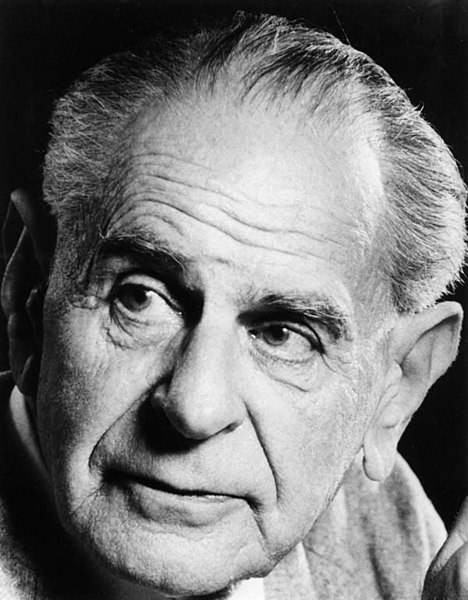
\includegraphics[width=.22\textwidth]{Figures/Karl_Popper.jpg}  
  \captionsetup{labelformat=empty}
  \caption{Karl Popper in the 1980's.} 
\end{center}
\end{wrapfigure}
\addtocounter{figure}{-1}

According to the Hypothetico-deductive method (H-D), a hypothesis is formulated, then relevant consequences are deduced, and finally we observe whether these consequences are false or true. Depending on these observations the hypothesis will be either falsified or confirmed.

Is important to note a key difference between confirmation and falsification. In step 4 of the \textbf{H-D method} we can infer the falsity of the hypothesis from the falsity of even a single one of the expected consequences. In contrast, in step 5 confirmation of the hypothesis is not inferred from the truth of even a large set of the consequences. Instead, we only increase our confidence on the hypothesis after finding that many consequences of the hypothesis are true. This difference is referred as the \textbf{asymmetry between confirmation and falsification}. Although a scientific theory can never be proved true by a finite amount of data, it can be proved false, or refuted by a single experiment.

\begin{quote}
``No amount of experimentation can ever prove me right; a single experiment can prove me wrong.'' --- Albert Einstein
\end{quote}

This asymmetry forms the basics of Karl Popper's (1902-1994) falsificationism.

\begin{itemize}
\tightlist
\item
  Propose falsifiable hypotheses.
\item
  Try to falsify these hypotheses with observable evidence.
\item
  Reject any falsified hypothesis as false.
\item
  Never accept any hypothesis as true - consider non-falsified hypotheses as ``not-rejected yet''.
\end{itemize}

\begin{quote}
One objection to this {[}the asymmetry between confirmation and falsification{]} holds that the asymmetry is an illusion, because whenever we refute a universal statement we thereby verify its negation. A universal statement ``All x are y'' is equivalent to ``There is no non-y x.'' Therefore, when we refute ``All apples are green'' we automatically verify ``There is a non-green apple.'' --- \citep{percival2015confirmation}
\end{quote}

Popper is quite radical in this last step. For him, confirmation places no role at all. One can never infer the truth of hypotheses - Popper argues - from the observations regarding their implications. Not even increase the confidence in the truth of the hypothesis. Popper hoped to avoid Hume's problem of induction by not employing induction in science. Popper thought that science was and should be deductive, and therefore that the lack of justification for inductive inferences was not as damaging for science. Below example is illustrative.

\begin{quote}
Suppose a scientist is testing the hypothesis that all pieces of metal conduct electricity. Even if every piece of metal they examine conducts electricity, this doesn't prove that the hypothesis is true, for reasons that we've seen. But if the scientist finds even one piece of metal that fails to conduct electricity, this conclusively refutes the theory. For the inference from `this piece of metal does not conduct electricity' to `it is false that all pieces of metal conduct electricity' is a deductive inference---the premise entails the conclusion. So if a scientist were trying to refute their theory, rather than establish its truth, their goal could be accomplished without the use of induction. --- \citep{okasha-pos}
\end{quote}

However, this view of science process could be rather limiting with respect to the actual scientific practice. First, it does not allow to distinguish between non-falsified hypotheses. Popper argues that obtaining evidence in favour of a given theory is generally easy, and holds that such \emph{corroboration} should count scientifically only if it is the positive result of a genuinely \emph{risky} prediction, which might conceivably have been false.

\begin{quote}
It is logically impossible to verify a universal proposition by reference to experience (as Hume saw clearly), but a single genuine counter-instance falsifies the corresponding universal law. In a word, an exception, far from ``proving'' a rule, conclusively refutes it. --- \citep{sep-popper}
\end{quote}

Second, in scientific practice hypotheses rarely have immediate observable consequences, they often require measurements or experiments to do so. For instance, the hypothesis ``this liquid contains 3 substances'' does not entail any direct observable consequence. We might use distillation or chromatography to test such hypothesis but this requires relying on \textbf{auxiliary hypothesis} (e.g.~the distillation machine works properly). This consideration quite changes the \textbf{H-D method} steps. Moreover, we never test a single hypothesis alone, but only in conjunction with various auxiliary hypotheses (Duhem-Quine Thesis). One relevant example is the work of Galileo Galilei and his reports of mountains on the moon and Jupiter satellites. Philosophers such as Cesare Cremonini refused to look through the telescope, arguing that the instrument itself might have introduced artefacts, producing a visual illusion. Therefore, Duhem-Quine thesis states that in order to falsify a hypothesis we must be confident that the responsible for falsity of the consequence are not the auxiliary hypotheses but the main hypothesis.

\begin{itemize}
\item
  \begin{enumerate}
  \def\labelenumi{\arabic{enumi}.}
  \tightlist
  \item
    Propose a hypothesis \(H\).
  \end{enumerate}
\item
  \begin{enumerate}
  \def\labelenumi{\arabic{enumi}.}
  \setcounter{enumi}{1}
  \tightlist
  \item
    Deduce observable consequences \(\{C_i\}\) from \(H\) in conjunction with auxiliary hypotheses \({AH_j}\)
  \end{enumerate}
\item
  \begin{enumerate}
  \def\labelenumi{\arabic{enumi}.}
  \setcounter{enumi}{2}
  \tightlist
  \item
    Test. Look for evidence that conflicts with the predicted consequences \(\{C_i\}\) in order to disprove \(H\).
  \end{enumerate}
\item
  \begin{enumerate}
  \def\labelenumi{\arabic{enumi}.}
  \setcounter{enumi}{3}
  \tightlist
  \item
    If \(\{C_i\}\) is false, infer that \(H \& \{AH_j\}\) is false, reformulate \(H\).
  \end{enumerate}
\item
  \begin{enumerate}
  \def\labelenumi{\arabic{enumi}.}
  \setcounter{enumi}{4}
  \tightlist
  \item
    If \(\{C_i\}\) is true, increase confidence in \(H \& \{AH_j\}\).
  \end{enumerate}
\end{itemize}

\begin{tipbox}

\textbf{Semantic Note:}

Note the difference between \emph{falsifiable} and \emph{falsified}.

\textbf{Falsifiability} is a quality of a hypothesis or a theory. Is the quality of a conjecture or hypothesis to be proven wrong. Some theories have no empirical implications. Popper claimed that astrology and Freud's psychoanalysis were not falsifiable. He argued that \emph{falsifiability} demarcates whether a theory is scientific or not (see the \href{https://plato.stanford.edu/entries/pseudo-science/}{demarcation problem} \citep{sep-pseudo-science}). Similarly, some hypotheses might be more falsifiable than others because they have more empirically testable implications. For example, Newton's law of gravitation is falsifiable (e.g.~it is falsified by ``The brick fell upwards when released'').

\textbf{Falsification} is the observation that an implication of a hypothesis is not true which implies (by \emph{modus tollens}) the falsity of the hypothesis. Hypothesis can only be falsified if they are falsifiable.

\begin{quote}
Falsification uses the valid inference modus tollens: if from a statement \(P\) we logically deduce \(Q\), but what is observed is \(\lnot Q\), we infer that \(P\) is false. For example, given the statement ``all swans are white'' and the initial condition ``there is a swan here'', we can deduce ``the swan here is white'', but if what is observed is ``the swan here is not white'' (say black), then ``all swans are white'' is false, or it was not a swan.
\end{quote}

\end{tipbox}

The take-away message from falsification is that despite proposing an unrealistically restrictive practice of science, it might be a useful inference method for scientists. However, they should be aware of its limitations and for instance, bear in mind the pitfalls of \emph{ad-hoc} modifications. (See negative weight in phlogiston theory \citep{phlogiston}). An \emph{ad-hoc} hypothesis is added to a theory to save it from being falsified. A modification is considered \emph{ad-hoc} if it reduces the falsifiability of the hypothesis in question.

\hypertarget{confirmation}{%
\subsection{Confirmation}\label{confirmation}}

Confirmation is the act of using evidence to justify increasing the confidence in the hypothesis.
Confirmation is not based on deductively valid inferences. For instance, in the \textbf{H-D method} we identify some \(C\) that is an implication of \(H\). \(H\) implies \(C\), then if \(H\) is true we conclude (by \emph{modus ponens}) that \(C\) is also true. Moreover, if we observe than \(C\) is false, then we conclude (by \emph{modus tollens}) that \(H\) is false as well. While these two inference rules are deductively valid, they do not tell us what to conclude if the implication \(C\) is true. There is no valid deductive rule that can be used for the case where \(H\) implies \(C\) and \(C\) is true. We cannot deduce anything from that.

\begin{verbatim}
Modus ponens     Modus tollens    Induction

H, then C        H, then C        H, then C
H                not C            C
-----------      -----------      =========
C                not H            H 
\end{verbatim}

Instead, any rule used here must amplify the information contained in the premises to infer the conclusions. Therefore we must make use of inductive inferences. Inductive inferences are fallible (inductions that fail are common e.g.~predicting the weather, stock investing). But fallibility comes in degrees and this degree is affected by the kind and quality of the evidence as well as the inference rule employed. Scientists have attempted to quantify confidence, most prominently by using probabilities. For instance, if an observation \(O\) confirms hypothesis \(H\), therefore we say that \(P(H|O)\) is greater than \(P(H|\lnot O)\) where \(P(H|O)\) means ``the probability of \(H\) given \(O\)''.

There is certain debate on this last point. Not everybody agrees that it makes sense to assign probabilities to hypotheses because they differ on the interpretation of the concept of probability. \textbf{Frequentists} interpret the probabilities as the frequencies of repeatable observable events. Therefore probabilities cannot be assigned to hypotheses since these are not events, nor observable or repeatable. Another problem is that probabilities are already used to express a property different from confidence. For instance, we may say that the probability of tails when throwing a coin is 50\%. But then someone may ask us how confident we are about our claim. Even if we can also answer that second question with a probability, is clear that these two numbers express different things.

\begin{tipbox}

\textbf{Note for data scientists!}

Is important to note the relevance of frequentist and Bayesian approaches in artificial intelligence. Both frequentist and Bayesian are statistical approaches to learning from data. But there is a broad distinction between the frequentist and Bayesian. The frequentist learning only depends on the given data, while the Bayesian learning is performed by the prior belief as well as the given data \citep{jun2016frequentist}.

The frequentist computes the probability of result or data \(D\) given hypothesis \(H\) is true, i.e.~\(P(D|H)\). In comparison, the Bayesian approach focus on the probability of hypothesis \(H\) when the result or data \(D\) occurs, i.e.~\(P(H|D)\) \citep{orloffcomparison}.

\end{tipbox}

Understanding that confirmation comes in degrees may help clarify the last step of \textbf{H-D method}. Observing \(C\) to be true, increases our degree of confidence that \(H\) is true. But why is this? A naïve answer to this question is that observing \(C\) confirms \(H\) because \(H\) is compatible with \(C\). But this seems rather weak justification. Indefinitely irrelevant implications could be inferred from a hypothesis. For instance:

\begin{verbatim}
I have pancreas cancer, then I have a pancreas
I have a pancreas    
---------
I have pancreas cancer
\end{verbatim}

A clear deductive consequence from this example is that indeed I have a pancreas. However, observing that I do have a pancreas should not confirm the claim that I have pancreas cancer. To solve this issue we should introduce a criteria for relevance to make sure that the chosen implications are relevant to the question. This is key part of the scientific process as this often depends on the domain knowledge we have about the matter we are investigating.

An additional problem to the compatibility issue, is that very many hypotheses are compatible with any given observation. This is called the problem of underdetermination.

\begin{figure}

{\centering 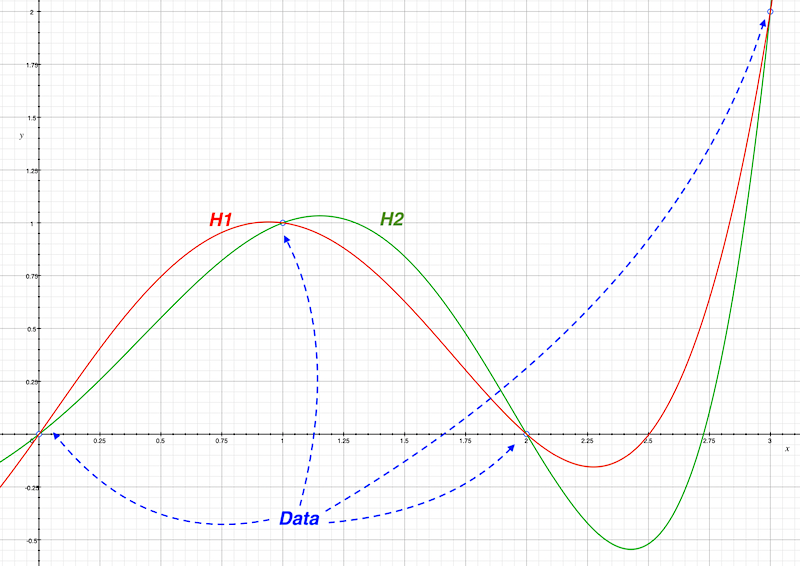
\includegraphics[width=0.75\linewidth]{Figures/underdetermination_small} 

}

\caption{The problem of underdetermination illustrated with a chart.}\label{fig:chart-underdetermination}
\end{figure}

\begin{tipbox}

\textbf{Note for data scientists!}

According to \emph{anti-realists}, there will always be multiple \emph{competing} theories about unobservable entities (e.g.~atoms) which can account for the data equally well. In other words, such theories are \emph{undetermined} by the empirical data. But then, how do scientists justify choosing one theory over another? \emph{Realists} often reply that aforementioned scenario is only possible in the trivial sense. In fact, scientists often struggle to find even \emph{one} theory that fits the data properly.

But why is this important for data scientists? Often you will find many ML models or solutions that fit your available data or fulfil your requirements, and yet you will have to decide which model/solution is best. If possible, validation with external data and other assessments must be conducted, but sometimes solutions are also chosen based on \emph{non-epistemic} values, such as making society more just or making money.

Is also important to notice how the problem of underdetermination relates to the popular \emph{No Free Lunch Theorem} which is very relevant in the Machine Learning community \citep{dotan2020theory}. For more on the NFL read \citep{domingos2015master}.

\end{tipbox}

\hypertarget{other-types-of-inference}{%
\section{Other types of inference}\label{other-types-of-inference}}

\begin{notebox}

\begin{center}
\textbf{Course Note:}

\end{center}

The following content is under construction but might as well be taught during the course. I hope to complete it on time.
This section will superficially tackle abduction and causal inferences and its relation to data science regarding non-monotonic logic.

\end{notebox}

\hypertarget{non-monotonic-logic-and-defeasible-reasoning}{%
\section{Non-Monotonic logic and defeasible reasoning}\label{non-monotonic-logic-and-defeasible-reasoning}}

In its epistemic sense, monotonicity expresses the fact that adding more premises to an argument allows you to derive all the same conclusions as you could with fewer \citep{sep-logic-nonmonotonic}. Specifically, under monotonic reasoning, if a conclusion \(p\) follows from a set of premises \(A\), (denoted as \(A\) \vdash \(p\)), adding another set of premises \(B\) doesn't alter the conclusion (i.e.~\(A ∧ B \vdash p\) also holds). Therefore, reasoning is \href{https://plato.stanford.edu/entries/logic-nonmonotonic/}{non-monotonic} when a conclusion supported by a set of premises can be retracted in the light of new information. Or in other words, we can infer certain conclusions from a subset of a set \(S\) of premises which cannot be inferred from \(S\) as a whole. Medical diagnosis fits very well under such definition.

\begin{figure}

{\centering 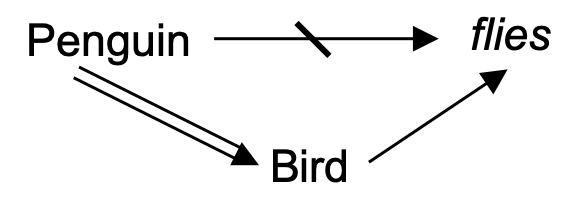
\includegraphics[width=0.33\linewidth]{Figures/PenguinFlies} 

}

\caption{Double arrows indicate non-defeasible inferences (hard fact), single arrows depict defeasible inferences, and strikethrough arrows denote a negation. It can be read as: Penguins are birds (no exceptions); Birds usually fly; and Penguins usually don’t fly.}\label{fig:tweety}
\end{figure}

Defeasible reasoning deals with tentative relationships between premises and conclusions, which can be \emph{defeated} by additional information, allowing for the retraction of inferences. For instance, while we may infer that Tweety flies based on the information that Tweety is a bird and the domain knowledge that birds generally fly, we can retract this inference when we learn that Tweety is a penguin. Tweety is indeed a bird but it cannot fly. Defeasible reasoning is not exempt from limitations, requiring from causal information to properly derive conclusions under certain scenarios. Consider, for example, this problem of Judea Pearl: if the sprinkler is on, then normally the sidewalk is wet, and, if the sidewalk is wet, then normally it is raining. However, we should not infer that it is raining from the fact that the sprinkler is on \citep{pearl2014probabilistic}. Conflicts may arise between hard facts and defeasible conclusions. For instance, both arguments in Figure \ref{fig:tweety} \(Penguin ⇒ Bird → flies\) and \(Penguin → ¬flies\) finish with a defeasible inference. The transitivity rule \((a → b, b → c) ⇒ a → c\) cannot be applied to the first argument. In this case, according to their specificity we can give priority to the argument with more a specific antecedent but is not always as trivial, and complex conflicts can remain unresolved.

\begin{quote}
Reasoning is defeasible when the corresponding argument is rationally compelling but not deductively valid. The truth of the premises of a good defeasible argument provide support for the conclusion, even though it is possible for the premises to be true and the conclusion false. In other words, the relationship of support between premises and conclusion is a tentative one, potentially defeated by additional information. --- \citep{sep-reasoning-defeasible}.
\end{quote}

\begin{quote}
Defeasible reasoning is a particular kind of non-demonstrative reasoning, where the reasoning does not produce a full, complete, or final demonstration of a claim, i.e., where fallibility and corrigibility of a conclusion are acknowledged. In other words, defeasible reasoning produces a contingent statement or claim. Defeasible reasoning is also a kind of ampliative reasoning because its conclusions reach beyond the pure meanings of the premises. Defeasible reasoning finds its fullest expression in jurisprudence, ethics and moral philosophy, epistemology, pragmatics and conversational conventions in linguistics, constructivist decision theories, and in knowledge representation and planning in artificial intelligence. --- Wikipedia
\end{quote}

\hypertarget{explanation}{%
\section{Explanation}\label{explanation}}

\begin{wrapfigure}{R}{.25\textwidth}  
 \begin{center}
    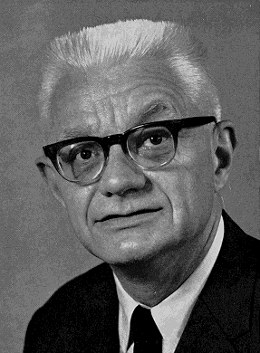
\includegraphics[width=.22\textwidth]{Figures/Carl_Gustav_Hempel.jpg}  
  \captionsetup{labelformat=empty}
  \caption{Carl Hempel (1905 - 1997).} 
\end{center}
\end{wrapfigure}
\addtocounter{figure}{-1}

At this point, many of you probably have already related data science to two of the goals of science: explanation and prediction. But how do they relate to one another? and what is a scientific explanation? Either to satisfy our natural curiosity or for a further purpose, science has always attempted to understand how the world works. The German philosopher Carl Hempel attempted to answer this question in the 1950s with what is known as the \emph{covering law} model of explanation. He stated that a scientific explanation is an answer given in response to \emph{explanation-seeking why-questions} (e.g.~why salt dissolves in water).

According to Hempel, explanations are structured like an argument, i.e.~a set of premises followed by a conclusion. Therefore, the conclusion of such an argument states that certain phenomenon occurs, e.g.~``salt dissolves in water''. On the other hand, the premises indicate why the conclusion is true. Then, the challenge lays in the relationship that should follow between such premises and the conclusion. For Hempel, the premises should all be true and entail the conclusion, i.e.~the argument should be deductive and \emph{sound}. Additionally, the premises should contain at least one general law (e.g.~all metals conduct electricity), a.k.a. \emph{laws of nature}. The name of the model comes from that fact that the phenomenon to be explained is ``covered'' by some general law.

\begin{enumerate}
\def\labelenumi{\arabic{enumi}.}
\tightlist
\item
  The \emph{explanandum} must be a valid deductive argument.
\item
  The \emph{explanans} must contain at least one general law actually needed in the deduction.
\item
  The \emph{explanans} must be empirically testable.
\item
  The sentences in the \emph{explanans} must be true.
\end{enumerate}

For instance, Newton explained the elliptical orbits of planets alluding a general rule (his law of universal gravitation) together with some minor assumptions. This example fits Hempel's model very well, but not all scientific explanations do.

\begin{verbatim}
General Law      (explanans)
Particular Facts (explanans)
---------
Phenomenon to be explained (explanandum)
\end{verbatim}

An interesting consequence of this model lays in the relationship between explanation and prediction. Hempel argued that these are two sides of the same coin. Whenever a phenomenon is explained with the help of a covering law, the laws and the particular facts we use could have allowed us to predict the occurrence of the phenomenon. Hempel expressed this by saying that every scientific explanation is potentially a prediction. Hempel argued that the opposite is also true: every prediction is potentially an explanation. \textbf{For Hempel, explanation and prediction are structurally symmetric}. For instance, the same information we could use to predict an animal species extinction before it happened will serve to explain that very same fact after it has happened.



\begin{figure}

{\centering 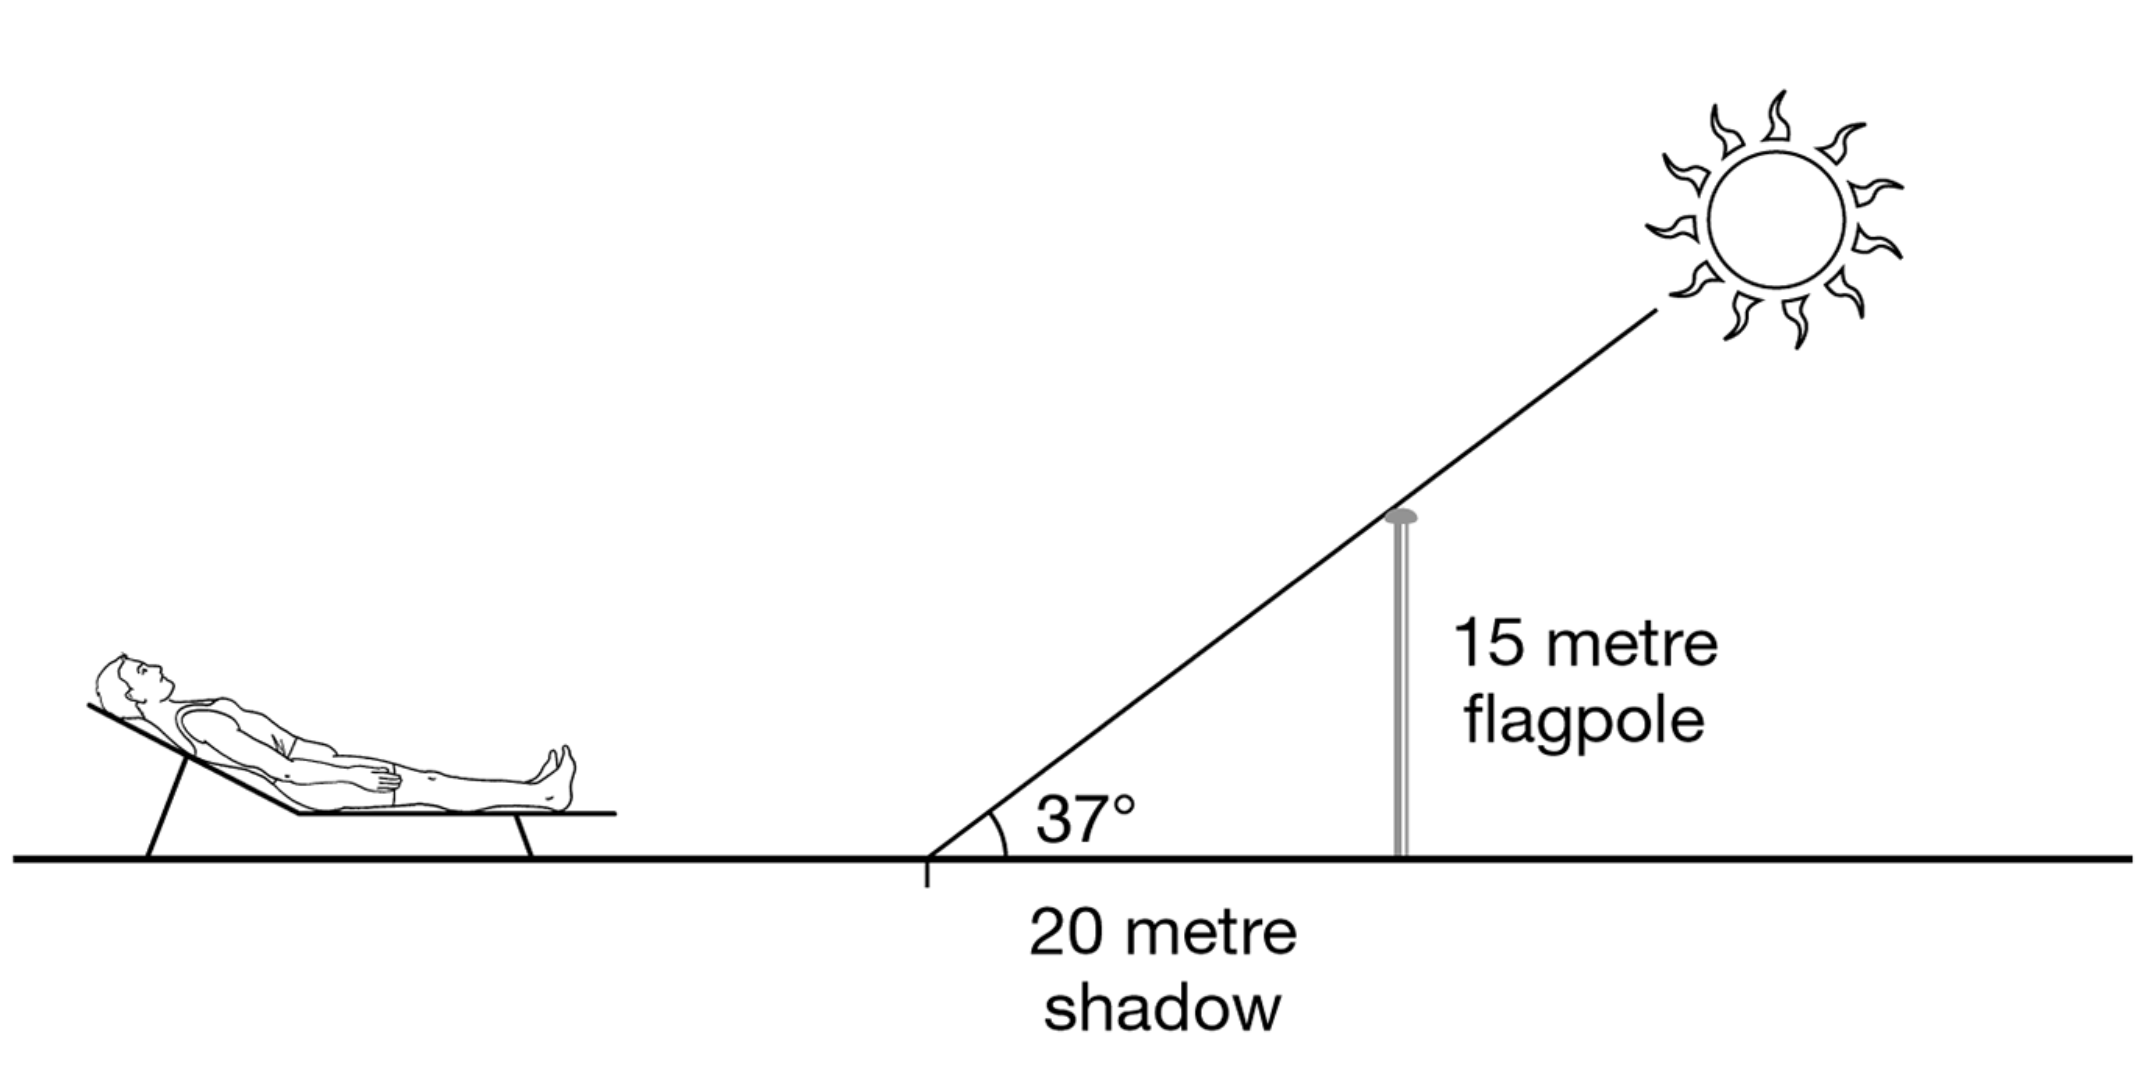
\includegraphics[width=0.75\linewidth]{Figures/flagpole} 

}

\caption{A 15-metre flagpole casts a shadow of 20 metres when the sun is 37° overhead. Figure from \citep{okasha-pos}.}\label{fig:flagpole}
\end{figure}

Hempel's model might be too liberal, as it faces a number of odd counterexamples. For example, consider Figure \ref{fig:flagpole}. In order to explain why the shadow is 20 metres long. Indeed, this is a \emph{explanation-seeking why-question} and a possible answer could be the following: The light rays from the sun hit the flagpole (15 metres high), the sun's elevation angle is 37° and light travels in straight lines. The trigonometric calculation \(tan(37°) = 15/20\) demonstrates that the flagpole will cast a shadow of 20 metres long. This example can be found in both \citep{rosenberg2019philosophy} and \citep{okasha-pos}.

\begin{verbatim}
General Law      (Light travels in straight lines)
General Law      (Trigonometric laws)
Particular Fact  (Flagpole is 15 metres high)
Particular Fact  (Sun's angle of elevation is 37°)
---------
Phenomenon to be explained (Shadow is 20 metres long)
\end{verbatim}

This explanation can be structured according to Hempel's schema and indeed fits Hempel's covering law model. However, when we swap the \emph{explanandum} with the particular fact that the flagpole is 15 metres high, a problem arises. The explanation still complies with the covering law pattern, but it would be rather odd to regard it as an explanation of why the flagpole is 15 metres high. In this case, we know that the height of the flagpole is not conditioned by the sun's angle of elevation but rather because it was manufactured with such height. We can \emph{calculate} or \emph{predict} its height but this height will not change upon the other variables, so they do not \emph{explain} the flagpole height.

\begin{verbatim}
General Law      (Light travels in straight lines)
General Law      (Trigonometric laws)
Particular Fact  (Shadow is 20 metres long)
Particular Fact  (Sun's angle of elevation is 37°)
---------
Phenomenon to be explained (Flagpole is 15 metres high)
\end{verbatim}

The moral of this example is that the concept of explanation showcases an important \textbf{asymmetry}. The length of the shadow can be explained by the height of the flagpole, given aforementioned general laws. But this does not happen in the other direction. In general, if \(x\) explains \(y\), then it will not be true that \(y\) explains \(x\) given the same laws and facts. Explanation is then an asymetric relation and Hempel's covering law model does not respect such asymmetry. Information that allow us to predict a fact before we know it does not serve to explain that very same fact after we know it, which \textbf{contradicts Hempel's thesis}.
The general conclusion is that a good explanation of a phenomenon should contain information that is relevant to the phenomenon's occurrence.

\hypertarget{explanation-and-causality}{%
\subsection{Explanation and causality}\label{explanation-and-causality}}

There are alternatives to the covering law model that help us understanding scientific explanation. For many, explaining a phenomenon is simply to say what caused it. Obviously, causality is also an asymmetric relation. If a faulty appliance caused a fire, then is clear that the fire did not cause the appliance's failure. The asymmetry of explanation derives from the asymmetry of causality.

However, the criticism against Hempel covering law is a bit unfair as he was an empiricist. Empiricists are sceptical about the concept of causality and argue that all our knowledge comes from experience. David Hume argued that is impossible to experience causal relations, and that causality is just what we humans project to understand the world.

There are however some examples were explanation and causality do not match. For example, to say that an object's temperature is the average kinetic energy of its molecules is to explain what temperature \emph{is}, but this does not yield the cause of such temperature.

The law \(PV = nRT.\) explains the temperature of a gas at equilibrium by appeal to its pressure and the volume it takes up. But volume and pressure cannot be \emph{causes} of temperature since all of them --- the temperature, the volume, and the pressure --- vary, in the way the law describes, instantaneously. The changes in volume at one time do not cause changes in temperature at a later time; instead, the change in temperature occurs during exactly the same interval that pressure is changing \citep{rosenberg2019philosophy}. The nature of causation is still an open debate, but most philosophers have agreed that causes somehow necessitate their effects and that mere regularity cannot express this necessity.

Another example, this time from \citep{book-of-why}, show us the gap between causal vocabulary and ordinary scientific vocabulary. Consider the problem of expressing the following causal relationship: The barometer reading \(B\) tracks the atmospheric pressure \(P\). We can write down the relationship as \(B = kP\), where \(k\) is a constant of proportionality. Thanks to algebra we can rewrite the equation in multiple ways such as: \(P = B/k\), \(k = B/P\), or \(B-kP = 0\). They mean the same and given two of the variables we can calculate the third. But in these equations there is no account of directionality. We cannot express that is the pressure which \emph{causes} the barometer to change and not the other way around. Similarly, we cannot express the fact that the singing of the rooster \emph{does not cause} the sun to rise. Why have scientists not captured such facts in formulas as is done in other areas like mechanics, geometry or optics? For a better understanding of causation and its role in data science I recommend you the Book of Why \citep{book-of-why}.

\begin{quote}
Data can tell you that the people who took a medicine recovered faster than those who did not take it, but they can't tell you why. --- Book of Why
\end{quote}

\begin{tipbox}

\textbf{Note for data scientists!}

In the biological and social sciences, instead of strict laws one finds statements of probabilities, or statistical regularities, and explanations that appeal to them. In the medical contexts, explanations often employ relations that are reported in statistical form in order to express causal relationships. For instance, it is accepted that smoking causes lung cancer because it is associated with a big increase in the probability of contracting lung cancer. Nonetheless, we know that \textbf{statistical correlation does not warrant causal connection}. There are some problems with the statement that smoking causes cancer. Some smokers never contract cancer, while some lung cancer victims never smoked. The latter issue is easy, smoking is not the only cause of lung cancer. However, the first problem is harder to tackle.

\begin{quote}
Smoking can be said to cause cancer if and only if, among all the different background conditions we know about (heredity, diet, exercise, air pollution, etc.), there is no correlation between smoking and a lower than average incidence of lung cancer, and in one or more of these background conditions, smoking is correlated with a higher incidence in lung cancer rates. --- \citep{rosenberg2019philosophy}
\end{quote}

\end{tipbox}

\newpage

\hypertarget{examples-1}{%
\section{Examples}\label{examples-1}}

\hypertarget{semmelweis}{%
\subsection{The problem is in your hands!}\label{semmelweis}}

\begin{wrapfigure}{R}{.25\textwidth}  
 \begin{center}
    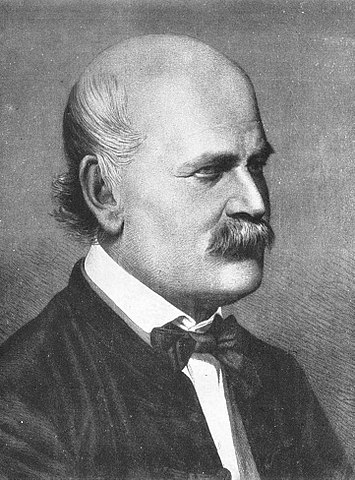
\includegraphics[width=.22\textwidth]{Figures/Semmelweis.jpg}  
  \captionsetup{labelformat=empty}
  \caption{Dr. Ignaz Semmelweis in 1860.} 
\end{center}
\end{wrapfigure}
\addtocounter{figure}{-1}

Ignaz Semmelweis, a Hungarian physician, was a member of the First Maternity Division at the Vienna General Hospital from 1844 to 1848. Semmelweis was distressed to find a big proportion of the women who delivered their babies contracted a serious and often fatal illness known as childbed fever. In 1844, 8.2\% of mothers died from the disease, 6.8\% in 1845 and 11.4\% in 1846. However, in the adjacent Second Maternity Division which had as many women as the first, the death toll was much lower (2.3\%, 2\% and 2.7\% respectively).

From this moment on, various explanations were considered, subjected to test and then rejected.

The first explanation attributed the issue to ``epidemic influences'' described as ``atmospheric-cosmic-telluric changes'' spreading over districts and causing childbed fever. This hypothesis did not explain why the first division had more cases than the second. Neither explained the lack of cases in the city of Vienna. Epidemics such as cholera are not so selective. Finally, Semmelweis notes that women who had to give birth in the street on their way to the hospital had a lower death rate than the average for the first division.

On a different view, overcrowding of the first division was proposed as a cause but Semmelweis pointed out that the second division was much crowded. Moreover, there were no differences regarding diet or general care of the patients.

In 1846, a commission was appointed to investigate the issue, which attributed the prevalence to injuries in the first division resulting from rough examination by medical students. Semmelweis refuted this view since: a) the injuries of birth itself are more extensive than those from the examination. b) midwives' examinations from the second division were similar. c) as a consequence of the commission the number of students was halved and the examinations were reduced to a minimum. The mortality increased.

After considering peculiar conjectures (e.g.~delivery position, priest visits), an accident gave Semmelweis the decisive clue. In 1847, a colleague of his received a puncture wound in the finger, from the scalpel of a student while performing an autopsy. His colleague died after an illness with similar symptoms to those observed in the victims of childbed fever. Note, that the role of micro-organisms had not yet been recognized at the time. Semmelweis ordered all medical students to wash their hands with a chlorinated lime solution before making examinations, especially after performing dissections in the autopsy room.

Mortality fell to 1.27\% in the First Division compared to 1.33\% in the second. In further support of his hypothesis, Semmelweis notes that midwives from the Second Division did not dissect cadavers. This also explained the ``street births'' low mortality since women were rarely examined as they already gave birth. Semmelweis concluded that the cause was infection by cadaveric material and putrid matter.

\begin{rnote}
Example and discussion extracted from Chapter 2 of \citep{hempel-pos}

\end{rnote}

\hypertarget{how-a-hypothesis-is-tested}{%
\subsubsection{How a hypothesis is tested}\label{how-a-hypothesis-is-tested}}

Some conjectures (e.g.~differences in diet, crowding or care) were trivial to test as their assumptions conflict with readily observable facts. Others were not as straightforward and required certain interventions. For example, changing the routine of the priest or the birth position. If the hypothesis \(H\) is true, then certain observable events \(I\) should occur (e.g.~drop in mortality) under specified circumstances (e.g.~lateral delivery position). Semmelweis experiment showed the test implication to be false, rejecting the hypothesis in consequence.

\begin{verbatim}
If H is true, then so is I.
But (as the evidence shows) I is not true.
---------------
H is not true.
\end{verbatim}

This is a good example of \emph{modus tollens} (see \ref{modus}). However, let us consider now the case where observation or experiment confirms the test implication \(I\). From the hypothesis that childbed fever is blood poisoning produced by cadaveric matter, Semmelweis infers that antiseptic measures will reduce mortality rates. Now, the experiment shows the test implication to be true. But this favourable outcome does not prove the hypothesis true.

\begin{verbatim}
If H is true, then so is I.
(as the evidence shows) I is true.
---------------
H is true.
\end{verbatim}

This reasoning is deductively invalid and referred to as the \emph{fallacy of affirming the consequent} (see \ref{modus}). The conclusion may be false even if its premises are true. Thus, even if many implications of a hypothesis have been confirmed by tests, the hypothesis may still be false.

\begin{verbatim}
If H is true, then so are I1, I2, ...
(as the evidence shows) I1, I2, ... are all true.
---------------
H is true.
\end{verbatim}

Above's argument still commits the fallacy. Note that although the many tests do not provide conclusive proof for a hypothesis, they provide at least some support or confirmation for it.

\begin{rnote}
Chapter 4 of \citep{hempel-pos} continues on this.

\end{rnote}

\begin{quote}
In the absence of unfavorable evidence, the confirmation of a hypothesis will normally be regarded as increasing with the number of favorable test findings. {[}\ldots{]} \textbf{the increase in confirmation effected by one new favorable instance will generally become smaller as the number of previously established favorable instances grows.} If thousands of confirmatory cases are already available, \textbf{the addition of one more favorable finding will raise the confirmation but little.}
\end{quote}

\begin{tipbox}

\textbf{Note for data scientists!}

Notice how Machine Learning (ML) models can also be affected by the previous statement. Many researchers blindly rely on the dogma \emph{the more data, the merrier} but is not just the amount of data that matters but also its variety. The greater the variety, the stronger the resulting support for the trained model.

\end{tipbox}

\hypertarget{wason}{%
\subsection{Wason selection task}\label{wason}}

\begin{figure}[hbtp]

{\centering 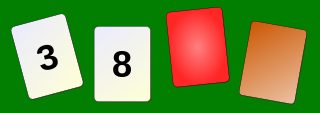
\includegraphics[width=0.25\linewidth]{Figures/wason_cards} 

}

\caption{Wason selection task or four-card problem.}\label{fig:wason-cards}
\end{figure}

Consider the following hypothetico-deductive reasoning problem created by Peter Cathcart Wason employing the logical rule of implication:

\begin{quote}
You are shown a set of four cards placed on a table, each of which has a number on one side and a colored patch on the other side. The visible faces of the cards show 3, 8, red and brown. Which card(s) must you turn over in order to test the truth of the proposition that if a card shows an even number on one face, then its opposite face is red?
\end{quote}

Hypothesis H: ``If a card shows an even number on one face, then its opposite face is red''

Test whether H is false. Which consequences of H do you need to consider - i.e.~which cards do you need to turn over? Under what conditions would this statement be false?

These are the possible situations:

\begin{itemize}
\tightlist
\item
  If the 3 card is red (or brown), that doesn't violate the rule. The rule makes no claims about odd numbers. (Denying the antecedent)
\item
  If the 8 card is not red, it violates the rule. (Modus ponens)
\item
  If the red card is odd (or even), that doesn't violate the rule. The red color is not exclusive to even numbers. (Affirming the consequent)
\item
  If the brown card is even, it violates the rule. (Modus tollens)
\end{itemize}

\begin{longtable}[]{@{}llr@{}}
\caption{Truth table for \(p \rightarrow q\). \textbf{(*)} In instances of \emph{modus ponens} we assume as premises that \(p \rightarrow q\) is true and \(p\) is true. Only one line of the truth table --- the first --- satisfies these two conditions (\(p\) and \(p \rightarrow q\)). On this line, \(q\) is also true. Therefore, whenever \(p \rightarrow q\) is true and \(p\) is true, \(q\) must also be true. \textbf{(**)} In instances of \emph{modus tollens} we assume as premises that \(p \rightarrow q\) is true and \(q\) is false. There is only one line of the truth table --- the fourth line --- which satisfies these two conditions. In this line, \(p\) is false. Therefore, in every instance in which \(p \rightarrow q\) is true and \(q\) is false, \(p\) must also be false.}\tabularnewline
\toprule
\(p\) & \(q\) & \(p \rightarrow q\) \\
\midrule
\endfirsthead
\toprule
\(p\) & \(q\) & \(p \rightarrow q\) \\
\midrule
\endhead
T & T & *T \\
T & F & F \\
F & T & T \\
F & F & **T \\
\bottomrule
\end{longtable}





There are two ways to face the problem and reach the solution. First, we can choose the cards based on \emph{modus ponens} and \emph{modus tollens} as follows: From \emph{modus ponens} we need to check the cards that are even. If even cards are not red, then the claim is false.

\begin{verbatim}
If even, then red. (claim)
even               (obs)
-----------------
Therefore, red.    (conclusion)
\end{verbatim}

From \emph{modus tollens} we need to check the cards that are not red i.e.~brown. If brown cards are even, then the claim is false.

\begin{verbatim}
If even, then red. (claim)
not red            (obs)
-----------------
Therefore, not even (conclusion)
\end{verbatim}

Another approach is to take the truth table of \(p \rightarrow q\) and take the case where \(p \rightarrow q\) is false - second line - i.e.~when \(p\) is true and \(q\) is false or for our case, when a card is even and its back not red (so brown). From this we need to take the cards that are \(p\) and \(\lnot q\) i.e.~even cards and brown cards.

\newpage

\hypertarget{u.s.a.-presidents}{%
\subsection{U.S.A. Presidents}\label{u.s.a.-presidents}}

\begin{figure}

{\centering 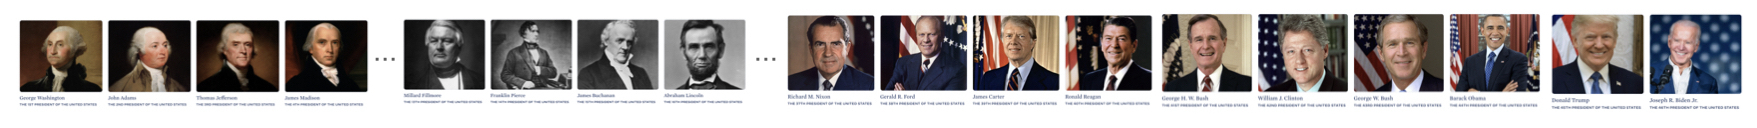
\includegraphics[width=1\linewidth]{Figures/usa_presidents} 

}

\caption{Presidents of the United States of America as of 2021.}\label{fig:us-presidents}
\end{figure}

Suppose we aim to predict whether the next president of the United States of America will be a woman or not. If we rely solely on the gender of previous presidents, by induction we will predict a zero chance. But by understanding how a person becomes a presidential candidate, and how previously became a candidate for their party, we can take into account the network of people involved in the process and recalculate our forecast with higher precision. In this case the rules are clearly defined in the law. Pouring these bits of domain knowledge into our model will show that chances are increasing over time. Encoding the rules behind the data heavily increased the robustness and precision of our model. Thanks to these rules our inference became deductive rather than inductive, since the conclusion necessarily follows from the premises; and as long as the premises are true the conclusion will also be true.

We can identify two issues in the first approach of our example: First, partial data can misrepresent the underlying phenomena that shapes the data, producing a model that does not resemble the real world. This is especially notable in the case of bias and confounders which are further aggravated by the lack of domain knowledge in designing the solutions. The second issue relates to induction. Contrary to deduction, where the truth of the premises guarantees the truth of the conclusion, inductive inferences are \emph{ampliative} --- since whose conclusions go beyond what is contained in their premises --- and their conclusions could be totally wrong even if infinitely many examples confirm them \citep{bergadano1991problem}. This \emph{ampliative} factor has also an amplifying effect over the partial data from which we infer a conclusion. In this case, considering only the final results of the elections amplified the bias derived from a partial collection of the data, reducing the chances of women being predicted as president to zero.

\begin{rnote}
From \citep{vega2021hume}.

\end{rnote}

\hypertarget{yersinia-pestis}{%
\subsection{Yersinia pestis}\label{yersinia-pestis}}

\begin{wrapfigure}{R}{.25\textwidth}  
 \begin{center}
    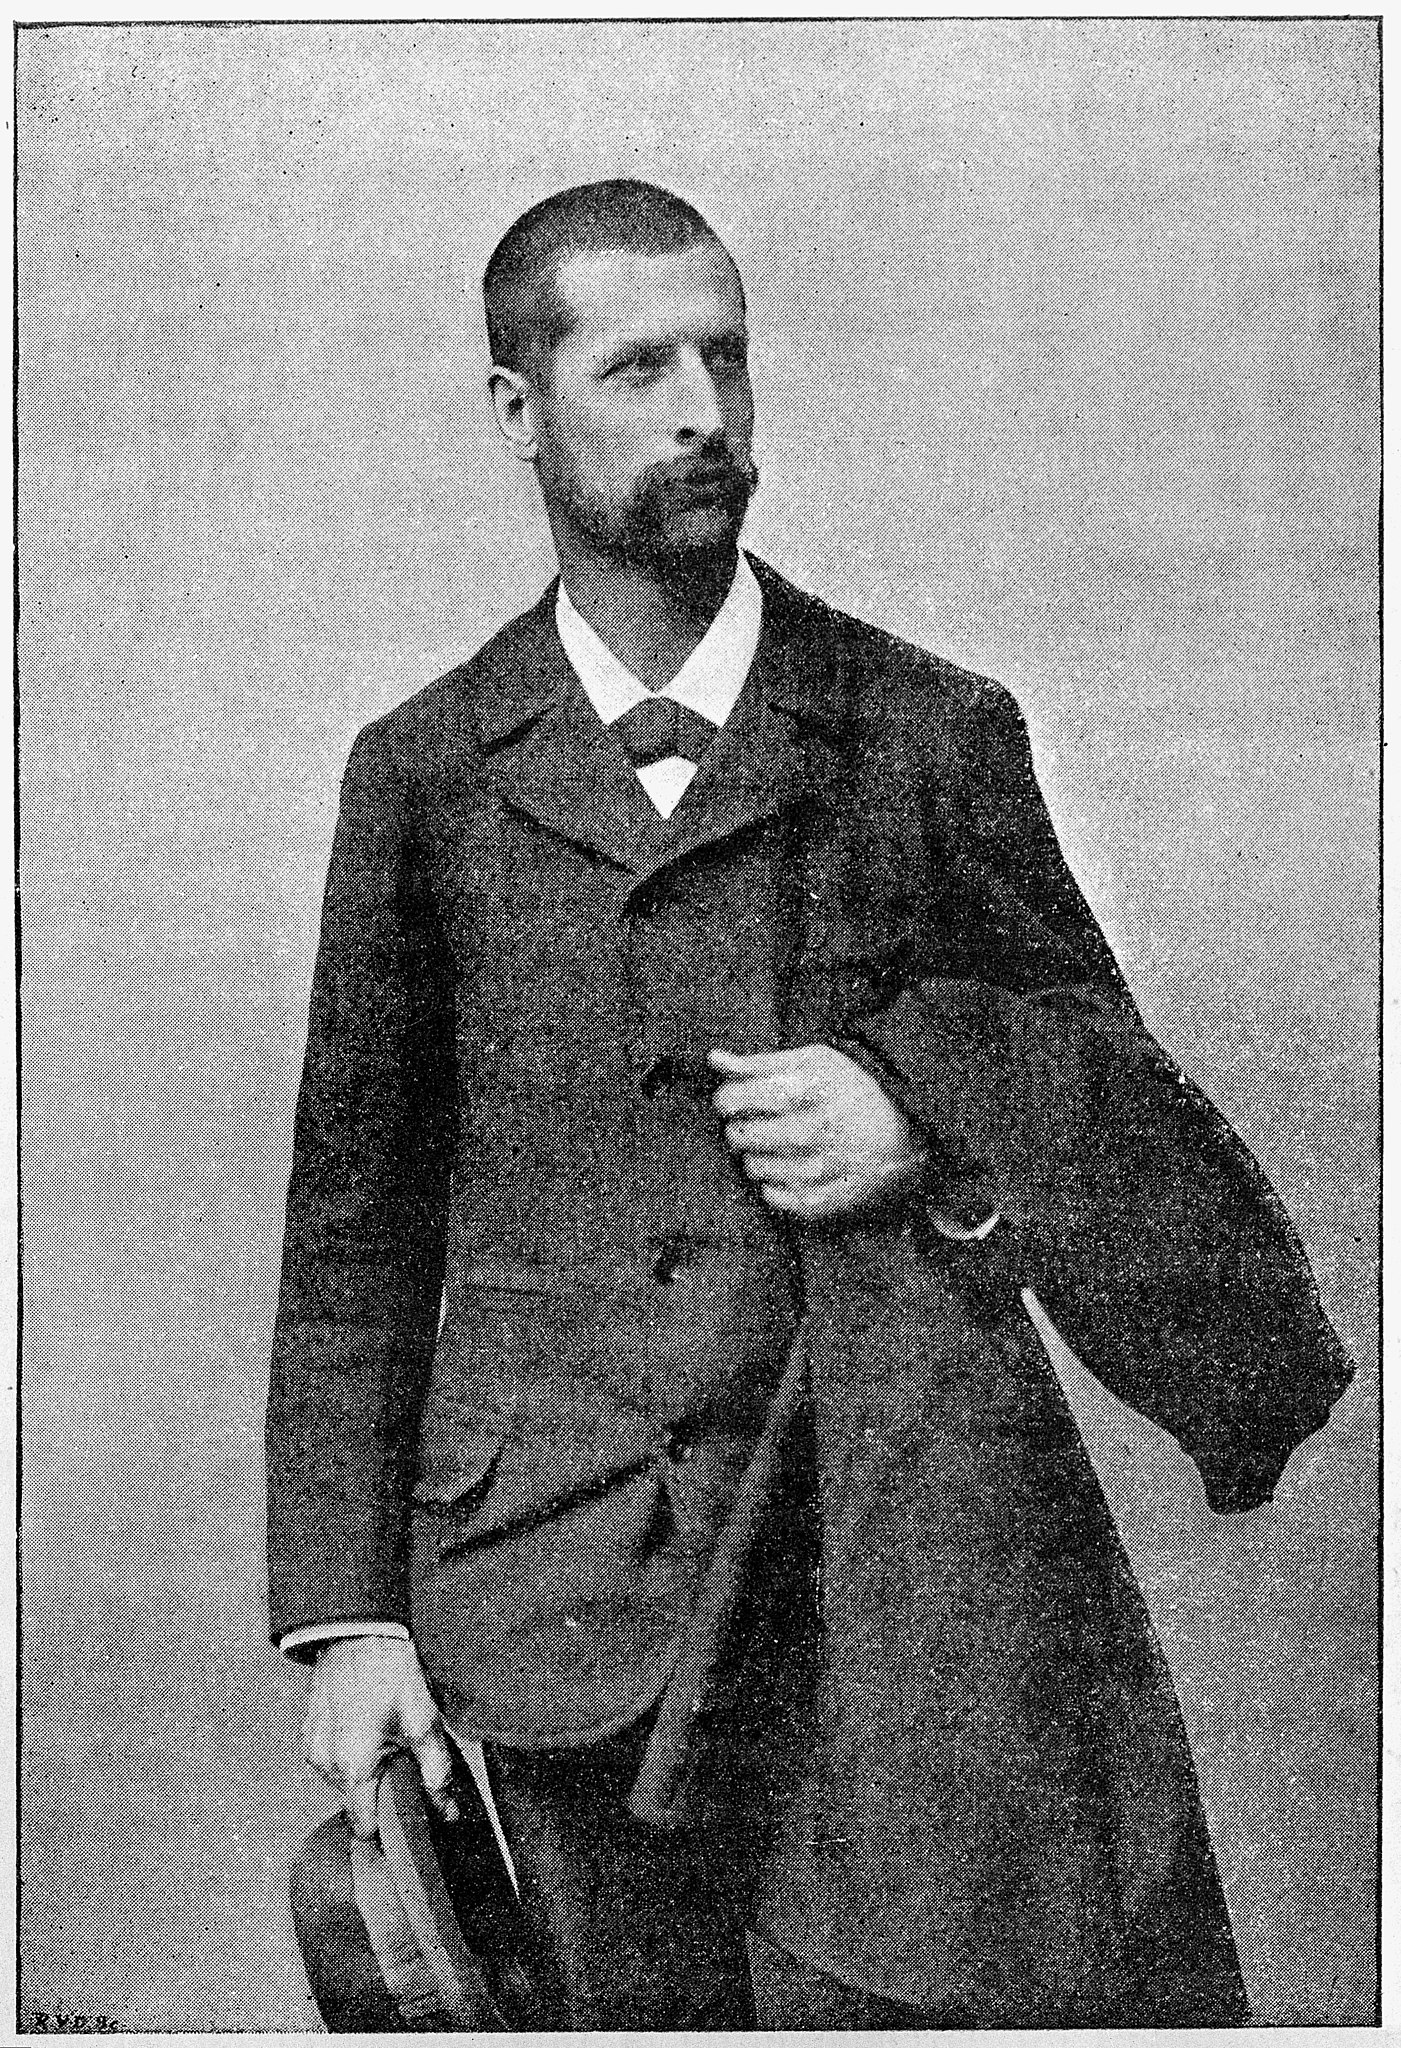
\includegraphics[width=.22\textwidth]{Figures/yersin.jpg}  
  \captionsetup{labelformat=empty}
  \caption{Alexandre Yersin.} 
\end{center}
\end{wrapfigure}
\addtocounter{figure}{-1}

This excerpt from Plague and Cholera is a great example of how laboratory conditions can act as an unintended auxiliary hypothesis that must be taken into account during research. It was 1894 in Hong Kong and all was set for an intellectual duel between Alexandre Yersin and Kitasato Shibasaburō that eventually unveiled the cause of the disease plague.

\begin{quote}
From the moment of his disembarkation in torrential rain, Yersin sees the bodies of plague victims lying in the street, in pools of standing water, in parks, aboard moored junks. British soldiers, acting on authority, remove the sick and empty their houses, pile everything up and set fire to it. {[}\ldots{]}
\end{quote}

\begin{quote}
`I notice many dead rats lying on the ground.' The first note scribbled by Yersin that evening concerns sewers spewing out decomposed bodies of rats. Since Camus, that has seemed obvious, but not then. {[}\ldots{]} By telegram, and as a concession to diplomacy, British governor Sir William Robinson gives Yersin explicit authority to come and study plague in Hong Kong. However, bad faith on the British side is clear to see, and it is even worse with the Japanese team under Shibasaburo Kitasato, who intends to reserve all autopsies for himself. {[}\ldots{]}
\end{quote}

\begin{quote}
Never again, in the history of humanity, will there be such an opportunity to become the person who vanquished plague. A few more weeks of devastation will mean a few thousand more bodies to study. {[}\ldots{]} Kitasato, though, has a handicap advantage. Not a single cadaver will be placed at Yersin's disposal. {[}\ldots{]}
\end{quote}

\begin{quote}
For Yersin's benefit he {[}Father Vigano{]} arranges, in just two days, to have a bamboo-framed, straw-covered hut erected near the Alice Memorial Hospital. With the matter of his living quarters and laboratory settled, Yersin installs a camp bed, unlocks the cabin trunk, and sets out microscope and test tubes. Vigano then greases the palms of the British sailors in charge of the hospital mortuary, where the bodies are stacked prior to being cremated or buried, and buys several from them. Yersin proceeds to ply his scalpel. {[}\ldots{]} `The bubo is quite distinct. In less than a minute I have it out and take it up to my laboratory. I make a quick preparation and place it under the microscope. One glance reveals a veritable mess of microbes, all similar. They are small stubby rods with rounded ends.' {[}\ldots{]} Yersin becomes the first human being to observe the plague bacillus, as Pasteur was the first to observe those of silkworm pebrine, ovine anthrax, chicken cholera and canine rabies.
\end{quote}

\begin{quote}
What Kitasato describes, having sampled organs and blood and disregarded the bubo, is the pneumococcus of a collateral infection, which he mistakes for the plague bacillus. Without luck, without chance, genius is nothing. The agnostic Yersin is blessed by the gods. Subsequent studies will show that one reason for Kitasato's failure is that he enjoyed the benefits of a proper hospital laboratory, including an incubator set at the temperature of the human body, a temperature at which pneumococcus proliferates, whereas the plague bacillus develops best at approximately twenty-eight degrees centigrade, the mean temperature in Hong Kong at that time of year and the temperature at which Yersin, with no incubator, conducts his observations.
\end{quote}

\begin{rnote}
From Plague and Cholera, by Patrick Deville. \citep{deville2014plague}

\end{rnote}

I absolutely recommend this book about Alexandre Yersin life. A Swiss-French physician and bacteriologist, pupil of Louis Pasteur, that trying to run away from himself became an agronomist and an explorer of the highlands of Vietnam and Cambodia.

\hypertarget{risks-of-induction-and-non-epistemic-values-in-ml}{%
\subsection{Risks of induction and non-epistemic values in ML}\label{risks-of-induction-and-non-epistemic-values-in-ml}}

I recommend the following \href{https://simonfischer.me/the-necessity-of-non-epistemic-values-in-machine-learning-modelling/}{blog post} from Simon Fischer. I copy a fragment here but the whole article is very interesting.

\begin{quote}
For example, when we think of the problem of \emph{filter bubbles} we are less and less confronted with opposing world views. Moreover, the idea that the future resembles the past, gives us examples of how Amazon has developed an algorithm for recruiting new staff which only hired males (Dastin, 2018). Even though the model might be correct from an epistemological point of view, such as accuracy or simplicity, it questions non-epistemic values, such as fairness. {[}\ldots{]}
\end{quote}

\begin{quote}
Another problem arises with regard to Popper's falsification approach. We cannot be sure what we have falsified: the hypothesis, the auxiliary assumptions, or even both? Consequently, under these considerations, it appears that the risks of drawing conclusions from machine learning outweigh the benefits. {[}\ldots{]}
\end{quote}

\begin{quote}
In the case of Amazon the false hypothesis and background assumptions were found rather quickly. But there could be more subtle biases around us which we are not yet aware. This again shows the twofold consequences in terms of inductive risk: The danger of scientists implementing these biases into the algorithms and the benefit of amplifying these biases, and thus making them visible to us. --- \citep{fischer_2020}
\end{quote}

\hypertarget{empirical-practices}{%
\chapter{Empirical Practices and Models}\label{empirical-practices}}

\hypertarget{overview-1}{%
\section{Overview}\label{overview-1}}

\begin{quote}
\emph{Empirical}: based on, concerned with, or verifiable by observation or experience rather than theory or pure logic.
\end{quote}

I would like to introduce this chapter in the same way the Book of Why \citep{book-of-why} introduces its fourth chapter ``Slaying the lurking variable''. During the times of Babylonian King Nebuchadnezzar (642 BC - 562 BC), one captive -- Daniel -- refused to eat royal meat offered by the King as part of their education and service in the court since it did not comply with his religious beliefs. Instead, Daniel asked to be fed on a vegetable diet. The overseer was reluctant as he thought the servants would lose weight and become weaker. Daniel proposed an experiment to convince his overseer. For ten days, one group of servants would be given a vegetable diet, while another group of servants would eat the king's meat. Then, the overseer would compare both groups and see that the vegetable diet did not reduce their strength. Of course, the experiment was a success, and the king was so impressed that he granted Daniel a favoured place in the court.

This example synthesizes the process of controlled experiments employed nowadays in experimental science. The overseer poses a question, \emph{will the vegetarian diet cause my servants to lose weight?}. There it is our hypothesis. To address the question, Daniel proposed a methodology. Divide the servants in two identical groups. Give one group a new treatment (e.g.~diet or a drug), while another group (control) remains under no special treatment. Of course, the two groups should be comparable and representative of some population in order to transfer the conclusions to the population at large. This process allowed Daniel to show the \emph{causal effect} (beware, we will tackle this in Chapter \ref{stats-abuse}) of the diet. Moreover, Daniel's experiment was prospective (in contrast to retrospective studies) as the groups were chosen in advance. Prospective controlled trials are a common characteristic of sound science. Still, Daniel did not think of everything, but we will see that in Chapter \ref{stats-abuse}.

\hypertarget{what-is-an-experiment}{%
\section{What is an experiment?}\label{what-is-an-experiment}}

Many data scientists believe their role should be limited to data analysis, but experiment design is fundamental for data collection, which conditions how the data must be analysed. Conclusions drawn from data can be biased or determined by decisions and errors taken during experiment design. Understanding this can help you spot issues during the data analysis and ask the right questions to your colleagues in charge of the experiments.

An experiment is an observation process in which we control background variables through manipulation, intervene on target variable (through manipulation) and observe the difference produced by such intervention thanks to measurements.

\begin{quote}
Experiment is the kind of scientific experience in which some change is deliberately provoked, and its outcome observed, recorded and interpreted with a cognitive aim. --- \citep{bunge2017philosophy}
\end{quote}

\hypertarget{observational-studies}{%
\subsection{Observational studies}\label{observational-studies}}

However, there are whole research areas were scientists cannot make experiments. For instance, astrophysics is mainly observational and theoretical as is not possible to manipulate the observed entities (e.g.~stars). It aims to find out measurable implications of physical models. Sometimes is not feasible, legal or ethical to conduct certain types of experiments, conducting observational studies instead. So, in \textbf{observational studies} there is no manipulation, no intervention on the target variable, neither control of background variables.

\hypertarget{natural-experiments}{%
\subsubsection{Natural experiments}\label{natural-experiments}}

\href{https://en.wikipedia.org/wiki/Natural_experiment}{\textbf{Natural experiments}} on the other side share the first two characteristics but is possible to control background variables (but not through manipulation though). See § \ref{john-snow} for an example. A major limitation of natural experiments when inferring causation is the presence of unmeasured confounding factors. Natural experiments are appealing for public health research because they enable the evaluation of events or interventions that are difficult or impossible to manipulate experimentally, such as many policy and health system reforms \citep{de2021conceptualising}.

\begin{quote}
For example the Canterbury earthquakes in 2010-2011 could be used to study the impact of such disasters because about half of a well-studied birth cohort lived in the affected area with the remainder living outside. {[}\ldots{]} More recently, the use of the term `natural' has been understood more broadly as an event which did not involve the deliberate manipulation of exposure for research purposes, even if human agency was involved. {[}\ldots{]} Natural experiments describing the study of an event which did not involve the deliberate manipulation of an exposure but involved human agency, such as the impact of a new policy, are the mainstay of `natural experimental research' in public health. --- \citep{de2021conceptualising}
\end{quote}

See Figure \ref{fig:diagram-experiments} for an schema depicting the conceptualisation of natural and quasi-experiments. Some authors differentiate between natural experiments and \emph{quasi-experiments}. In a quasi-experiment, the criterion for group assignment of the study units (e.g.~study participants) is selected by the researchers, whereas, in a natural experiment, the assignment occurs \emph{naturally}, without the intervention of the researchers.

\begin{quote}
Quasi-experiment: A quasi-experiment is an empirical interventional study used to estimate the causal impact of an intervention on target population without random assignment. Quasi-experimental research shares similarities with the traditional experimental design or randomized controlled trial, but it specifically lacks the element of random assignment to treatment or control. Instead, quasi-experimental designs typically allow the researcher to control the assignment to the treatment condition, but using some criterion other than random assignment. Quasi-experiments are subject to concerns regarding internal validity, because the treatment and control groups may not be comparable at baseline. In other words, it may not be possible to convincingly demonstrate a causal link between the treatment condition and observed outcomes. This is particularly true if there are confounding variables that cannot be controlled or accounted for. --- Wikipedia on \citep{rossi1985evaluation} and \citep{dinardo2010natural}.
\end{quote}



\begin{figure}

{\centering 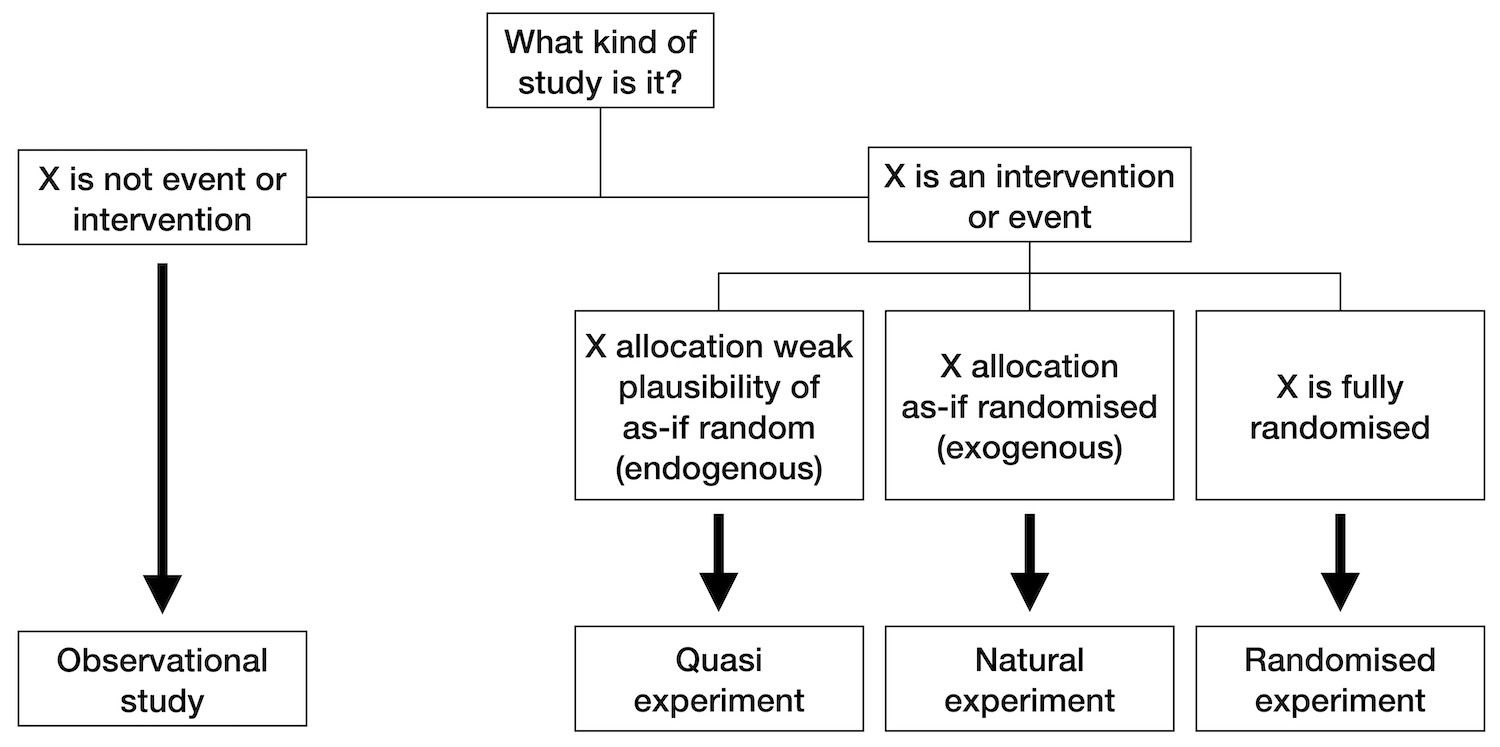
\includegraphics[width=1\linewidth]{Figures/natural-experiments} 

}

\caption{Diagram depicting the conceptualisation of natural and quasi-experiments within the evaluation framework of Thad Dunning. Re-drawn from \citep{de2021conceptualising}. Note that the same article provides three additional conceptualisations from different frameworks. For example, a different conceptualisation makes a distinction between quasi and natural experiments, arguing that natural experiments describe unplanned events whereas quasi-experiments describe events that are planned (but not controlled by the researcher).}\label{fig:diagram-experiments}
\end{figure}

\begin{quote}
Dunning takes this concept further and defines a `natural experiment' as a quasi-experiment where knowledge about the exposure allocation process provides a strong argument that allocation, although not deliberately manipulated by the researcher, is essentially random, referred to as `as-if randomization'. --- \citep{de2021conceptualising}
\end{quote}

\begin{tipbox}

\textbf{Definitions:}

\textbf{Target variables}: The target variable of a dataset is the feature of a dataset about which you want to gain a deeper understanding. They also receive the name ``dependent variables'' because, in an experiment, their values are studied under the supposition or demand that they depend, by some law or rule (e.g., by a mathematical function), on the values of other variables. The dependent variable is the \emph{effect}. Its value depends on changes in the independent variable.

\textbf{Independent variables}: It is a variable that stands alone and isn't changed by the other variables you are trying to measure. The independent variable is the \emph{cause}. Its value is independent of other variables in your study.

\textbf{Background variables}: An explanatory variable that can affect other (dependent) variables but cannot be affected by them. For example, one's schooling may affect one's subsequent career, but the reverse is unlikely to be true.

\end{tipbox}

We can recognise five elements in the observation process: the \emph{object} of observation; the \emph{subject} (or observer) and its perceptions; the \emph{circumstances} of observation (e.g.~environment of object and subject); the observation \emph{media} (e.g.~senses, instruments, procedures); and the body of \emph{knowledge} used to relate all the previous elements. The last two can be grouped into \emph{tools} (concrete and conceptual). So, an observation statement has the form ``\(w\) observes \(x\) under \(y\) with the help of \(z\)''. \citep{bunge2017philosophy}

\hypertarget{observability}{%
\subsubsection{Observability}\label{observability}}

We can try to define observability by stating that a fact is \emph{observable} ``only if there exists at least one subject, one set of circumstances, and one set of observation tools, such that the fact can appear to the subject armed with those tools under those circumstances'' \citep{bunge2017philosophy}. This definition is rather unsatisfactory since someone could claim the existence of ghosts or aliens. We should define what is objectively observable. Then, \(x\) is observable only if there exist at least one recording instrument \(w\), one set of circumstances \(Y\), and one set of observation tools \(Z\), such that \(w\) can register \(x\) under \(y\) helped by \(z\). Here we have eliminated the possibility of the subject's perceptual delusions, but devices (e.g.~a camera) have limitations too.

Observations are often expressed in the form of a rule so that other researchers can reproduce their results under similar conditions. Some facts cannot be repeated, such as the eruption of a volcano or a supernova. So very often, we expect results of the same kind to be reproducible by observers. Exact duplication is desirable but not always achievable. Even independent observers may make the same wrong observations due to faulty equipment or false hypotheses.

\hypertarget{indicators}{%
\subsubsection{Indicators}\label{indicators}}

Most facts we know about are indirectly observable, i.e.~we infer them through an intermediary. For instance, the wind is not directly observable but inferred from bodies apparently moved by it. We \emph{objectify} an unobservable fact by establishing its relationship to some perceptible fact(s) that serve us as an \emph{indicator} of the fact. In other words, hypotheses are made concerning unperceived facts and tested through evidence consisting of data about other directly observable facts, assuming that the latter are \textbf{collaterally connected with} or \textbf{effects} of the former. Of course, that such relationship should hold is as well a hypothesis (see Figure \ref{fig:indicator}).



\begin{figure}

{\centering 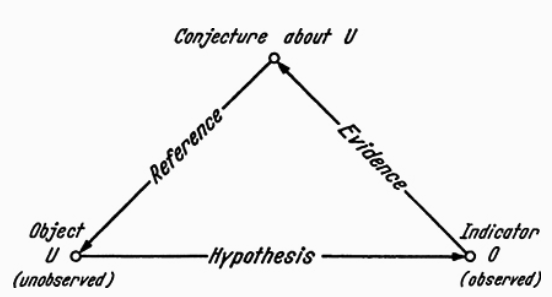
\includegraphics[width=0.5\linewidth]{Figures/indicator} 

}

\caption{The physical object-indicator relation, is expressed by a hypothesis enabling us to infer the object from observations made on its indicator. Figure extracted from \citep{bunge2017philosophy}.}\label{fig:indicator}
\end{figure}

\hypertarget{data-and-evidence}{%
\subsubsection{Data and Evidence}\label{data-and-evidence}}

Every evidence is a \emph{datum} but not every datum constitutes \emph{evidence}. What turns a datum into evidence is that is relevant to some idea, that it makes sense under some theory or body of knowledge. In particular, we believe a datum constitutes an evidence in favour of a theory and assign the theory some \emph{credence} because it justifies or predicts that evidence. The evidence must be related to a specific hypothesis, and this relationship is justified because of a body of theoretical knowledge. In fact, no evidence is absolute. Consider the following example from \citep{bunge2017philosophy}:

\begin{quote}
The observed deviation of a magnetic needle in the vicinity of an electric circuit (datum \(e\)) supports the hypothesis \(h_x\) that electricity is flowing through the circuit, on the theory \(⊤_1\) that electric currents produce magnetic fields which in turn interact with the fields of magnetic needles. But exactly the same datum \(e\) might be taken as an evidence in favour of the rival hypothesis \(h_2\) that a big magnet somewhere nearby has been switched on, on the theory \(⊤_2\) that magnets can interact directly with one another. The given datum is then \emph{ambiguous} and only an independent checking of \(h_x\) and \(h_2\), i.e.~a test independent of \(e\), will enable us to reach a decision between the two rivals.
\end{quote}

Importantly, the characteristics that make data count as evidence must be agreed prior to observation and on the basis of theory. Sometimes a scientist may obtain data that seems incompatible with a theory. Instead of getting rid of such data (or the theory), the scientist will attempt to reproduce the data and assess whether is anomalous data (e.g.~due to a faulty instrument) or not. The \emph{raw} data may contain any information, but \emph{refined} data should express only relevant and useful information for the problem at hand. Of course, some information is always lost in the process. In consequence, the refinement process is irreversible. Data are \emph{means} rather than \emph{ends} and we aim to systematise data in order to disclose patterns on it. For this reason \emph{noise} must be removed. The systematization of refined data may involve displaying information in graphs or tables as well as arranging information in data structures such as matrices.

\hypertarget{field-laboratory-and-simulation-experiments}{%
\subsection{Field, laboratory and simulation experiments}\label{field-laboratory-and-simulation-experiments}}

\hypertarget{field-experiments}{%
\subsubsection{Field experiments}\label{field-experiments}}

In contrast to observational experiments, \textbf{field experiments} randomly assign the sampling units (e.g.~study participants) into two groups (treatment and control) to test causal relationships. The same conditions are maintained for both groups only varying the intervention on the factor of interest (e.g.~two parts of soil (fertilized/unfertilized)). The background variables are considered as given and not manipulated.

\begin{itemize}
\tightlist
\item
  No manipulation.
\item
  No intervention on the target variable.
\item
  Control for the background variable (but not through manipulation).
\end{itemize}

In the example (see Figure \ref{fig:fertiliser}), the background variables are controlled, we do not alter the soil, the number of hours of sun light received by the two groups of plants, nor the watering conditions. The only intervention is giving fertiliser to one side of the field. In this case, the seeds can be randomly assigned the treatment (fertiliser) or control groups.

\begin{figure}

{\centering 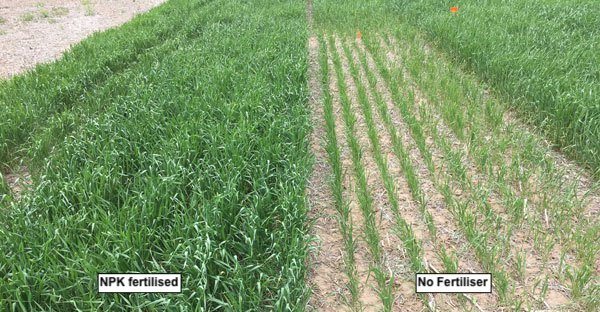
\includegraphics[width=0.66\linewidth]{Figures/crop} 

}

\caption{Fertiliser experiment.}\label{fig:fertiliser}
\end{figure}

\textbf{Potential threats to internal validity}

\begin{itemize}
\item
  Excludability: The assumption of excludability states that the randomization does not affect outcomes through other variables than the reception of the treatment. If this assumption is violated, the causal effect identified in a study is a combination of the treatment and other variables \citep{hansen2020systematic}. For instance, that the two fields do not receive the same amount of light.
\item
  Interference: Interference occurs when experimental units alter each other's outcomes. This generates a bias that precludes the proper estimation of causal effects by the reseachers.
\item
  Attrition: Attrition occurs when outcome data are missing. Attrition becomes a problem for causal inference when two conditions are present: (1) units with missing outcomes differ systematically on the outcome from those that are not missing and (2) attrition is different in experimental groups. There is greater potential for attrition in field experiments than in laboratory experiments because field experiments confer less control \citep{hansen2020systematic}. For instance, some participants may leave a study if they do not get any improvement.
\end{itemize}

\hypertarget{laboratory-experiments}{%
\subsubsection{Laboratory experiments}\label{laboratory-experiments}}

On the other side, \textbf{laboratory experiments} construct the same background conditions in both groups manipulating the environment (lab settings) and varying the intervention on the factor of interest. Background conditions are controlled through manipulation. For instance, temperature, pressure, humidity can be controlled for a fertiliser trial. Laboratory experiments tend to have higher internal validity, but at the cost of lower external validity (generalistation), owing to the artificial setting in which the study is conducted may not reflect the real world.

\hypertarget{simulation-experiments}{%
\subsubsection{Simulation experiments}\label{simulation-experiments}}

Finally, \textbf{simulation experiments} are constructions representing a real system on a computer to perform interventions. This type of experiments are done when it is not feasible to experiment on the real entities (e.g.~climate simulations or geological simulations). The important consideration is that all interventions and manipulations are performed on the computer representation instead of the real target itself.

\hypertarget{wrap-up}{%
\subsubsection{Wrap-up}\label{wrap-up}}

Therefore, an experiment is a controlled observation in which the observer manipulates the real variables (independent variables) that are believed to influence the outcome (dependent variable), both for the purpose of intervention and control. The following article provides a good description of the \href{https://opentextbc.ca/researchmethods/chapter/experiment-basics/}{basics of experiments}.

In Chapter \ref{stats-abuse} we will see some examples of experimental errors (e.g.~confirmation bias, selection bias, etc) as well as examples of statistical abuse. All in all, the experiment process is also a craft which entails learning from previous experiments (ours and others), as well as applying all available knowledge (theoretical and experimental) for the design of experiments.

\begin{tipbox}

\textbf{Definitions:}

\textbf{Repetition}: An experiment is repeatable if enough information is provided about the used data and the experiment methods and conditions. With such information, it should be possible to repeat the experiment.

\textbf{Reproduction}: An experiment is considered as reproduced if the repetition of the experiment yields the same result. For instance, in computer science, reproducing involves using the original data and code.

\textbf{Replication}: An independent experiment, in the spirit of the original experiment produces the same result. For example, in computer science replication entails collecting new data and use similar methods to reach similar conclusions in answer to the same scientific question. Or implementing a new software following similar design principles and reaching similar results.

\end{tipbox}

\hypertarget{how-to-evaluate-experiment-success}{%
\subsection{How to evaluate experiment success}\label{how-to-evaluate-experiment-success}}

Very often, success is not defined by a single goal or metric. For instance, the best car is not always the fastest car. In fact, there are many other values to bear in mind, such as gasoline consumption, pollution, ease of manufacture, etc. Similarly an experiment success is rarely assessed with a single metric in mind.

Moreover, some metrics must not be degraded, often called \textbf{guardrail metrics}. This type of metrics can include security, speed, robustness, etc. But very often include \emph{non-epistemic values} too. In this context, non-epistemic values are metrics not directly related to the instance to be designed, such as fairness, justice, or making money (or saving it), in contrast to metrics that make the instance at issue \emph{internally} or \emph{intrinsically} better (e.g.~speed). For instance, a car is not necessarily a better car depending on its price if what is judged is the \emph{car itself} in isolation, but a low price might make it easier to sell. In another example, the fastest data processing system might not necessarily be the best choice since other requirements must be considered too (e.g.~ease of use).

A non-epistemic value that is always at stake is money, or in a different shape, OPEX (operational expenditure) and CAPEX (capital expenditure). Very often, they condition other metrics, such as performance (e.g.~use less/worse resources) or safety (e.g.~employ less/worse materials). For example, I had the opportunity to work on the design of enterprise log processing systems. In this case, we wanted to maximise speed while reducing resources, as mid-sized companies often wish to reduce the number of servers deployed, which ultimately affects their operational costs (e.g.~space and electricity). Most commercial solutions scale horizontally, requiring the use of on-site server clusters to handle large amounts of data (at prohibitively high prices) or cloud-hosted clusters (impractical due to data protection). Our proposal optimised vertical scalability and coped with tens of millions of events per second with a single server. But of course, such an approach was specifically designed for a particular task, in contrast to the flexibility offered by commercial alternatives.

In data science, success should be defined by how well the analysis answers the research questions. For this reason, setting the research questions at the very beginning of the process remains crucial. They not only determine the data analysis but, more importantly, the data collection design. However, very frequently, the data science process starts with a given dataset. Still, it is essential to assess if the collected data can answer the posed questions.

\hypertarget{scientific-models}{%
\section{Scientific models}\label{scientific-models}}

Scientific models are widespread and varied. These include scale models (e.g.~plane models for aerodynamic studies), laboratory animals (e.g.~mice for drug trials), simulation models (e.g.~computational model for weather forecast). In all the previous cases, a model is made to replace or to stand in for what we are ultimately interested in. Models are characterised by being \textbf{representations}, containing \textbf{idealisations}, being \textbf{purpose dependent}, and \textbf{ready to be manipulated}.

\begin{quote}
Typically models are representations in which details, that appear inessential for intended uses, are omitted. A model is intended to represent the real thing in certain significant aspects. --- Guy Orcutt
\end{quote}

\begin{figure}

{\centering 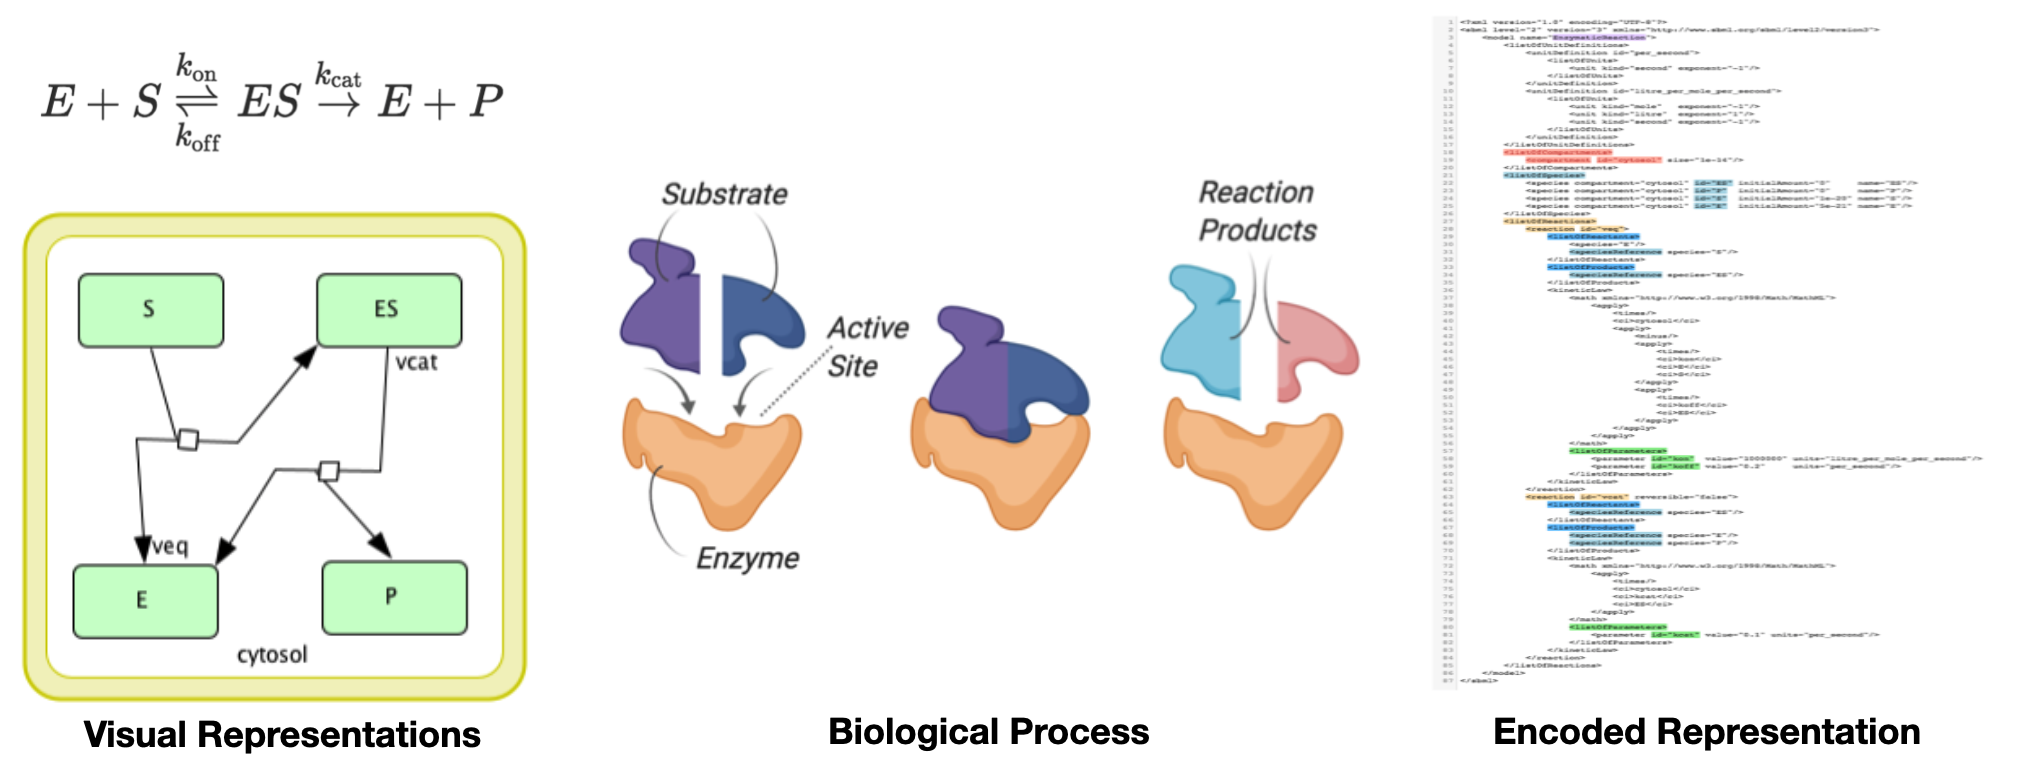
\includegraphics[width=1\linewidth]{Figures/sbml_model} 

}

\caption{Different representations of a biological process. On the right side, the process is encoded in a XML file in Systems Biology Markup Language (SBML) format. }\label{fig:sbml-model}
\end{figure}

\begin{quote}
We shall be concerned with model objects and theoretical models as hypothetical sketches of supposedly real, though possibly fictitious, things or facts. Thus a fluid may be modeled as a continuum endowed with certain properties, such as compressibility and viscosity. Such a model object may be grafted onto any of a number of general theories, say classical mechanics, or general relativistic mechanics. Likewise, a learning organism may be modeled as a black box equipped with certain input and output terminals, and this model object may then be expanded into a hypothetico-deductive system. In either case a specific theory, or theoretical model, of a concrete (or supposedly concrete) object, results. What can be subjected to empirical tests are such theoretical models: on the other hand general theories, being unconcerned with particulars, remain empirically untestable unless enriched with models of their referents. --- \citep{bunge2012method}
\end{quote}

For instance, a physical model of DNA on a table represents the real DNA. Obviously, such a model is not a piece of real DNA. It is made of something else (e.g.~plastic) and at a different scale. In this case, such a model is useful for pedagogic purposes. Although there are clear differences between models and targets, the key relationship is that \textbf{a model represents (in some way) the target}. From the methodological point of view, we must justify why to represent targets with models instead of investigating the targets themselves?. Possible answers include physical impossibility, costs, ethical and legal reasons, etc. However, very often the main justification to employ models is that targets are very complex. Therefore, employing a model that simplifies the target complexity might allow us to get a better understanding of the main factors operating in the target system. Our cognitive limits very often determine how we investigate complex systems, starting with a simpler model and increasing its complexity as we gain understanding.

\begin{quote}
A schematic representation of an object may be called a model object. If the represented object (or referent) is concrete or physical, then its model is an idealization of it. The representation may be pictorial, as in the case of a drawing, or conceptual, as in the case of a mathematical formula. It may be figurative, like the ball-and-spoke model of a molecule, of semisymbolic, as in the case of the contour map of the same molecule; or finally symbolic like the hamiltonian operator for that same object. --- \citep{bunge2012method}
\end{quote}

Therefore, we are intentionally choosing or building a model that differs from the target in some properties. Precisely because of this condition, we cannot assume that whatever is the case in the model is also the case in the target. \textbf{Models come with idealisations.} Not bearing in mind this key condition of the models can lead us to produce false claims about the target.

\begin{quote}
\begin{itemize}
\tightlist
\item
  \textbf{Idealized models.} Idealized models are models that involve a deliberate simplification or distortion of something complicated with the objective of making it more tractable or understandable. Frictionless planes, point masses, completely isolated systems, omniscient and fully rational agents, and markets in perfect equilibrium are well-known examples. Idealizations are a crucial means for science to cope with systems that are too difficult to study in their full complexity.
\item
  \textbf{Scale models.} Some models are down-sized or enlarged copies of their target systems (Black 1962). A typical example is a small wooden car that is put into a wind tunnel to explore the actual car's aerodynamic properties.
\item
  \textbf{Phenomenological models.} Phenomenological models have been defined in different, although related, ways. A common definition takes them to be models that only represent observable properties of their targets and refrain from postulating hidden mechanisms and the like.
\item
  \textbf{Exploratory models.} Exploratory models are models which are not proposed in the first place to learn something about a specific target system or a particular experimentally established phenomenon. Exploratory models function as the starting point of further explorations in which the model is modified and refined.
\item
  \textbf{Models of data.} A model of data (sometimes also ``data model'') is a corrected, rectified, regimented, and in many instances idealized version of the data we gain from immediate observation, the so-called raw data. Characteristically, one first eliminates errors (e.g., removes points from the record that are due to faulty observation) and then presents the data in a ``neat'' way, for instance by drawing a smooth curve through a set of points. These two steps are commonly referred to as ``data reduction'' and ``curve fitting''.
  --- \citep{sep-models-science}
\end{itemize}
\end{quote}

\hypertarget{the-models-of-the-atom}{%
\subsection{The models of the atom}\label{the-models-of-the-atom}}

For example, Bohr's model of the atom assumes that electrons orbit the atomic nucleus in circles. The success of such a model relied that the Bohr assumptions reproduced the series that fitted the hydrogen emission spectra. In 1913 it predicted the correct frequencies of the specific colours of light absorbed and emitted by ionised helium. One could say that Bohr was very lucky as despite his model is wrong in some ways, it also has some bits of truth, enough for his predictions about ionised helium to work out.



\begin{figure}[hbtp]

{\centering 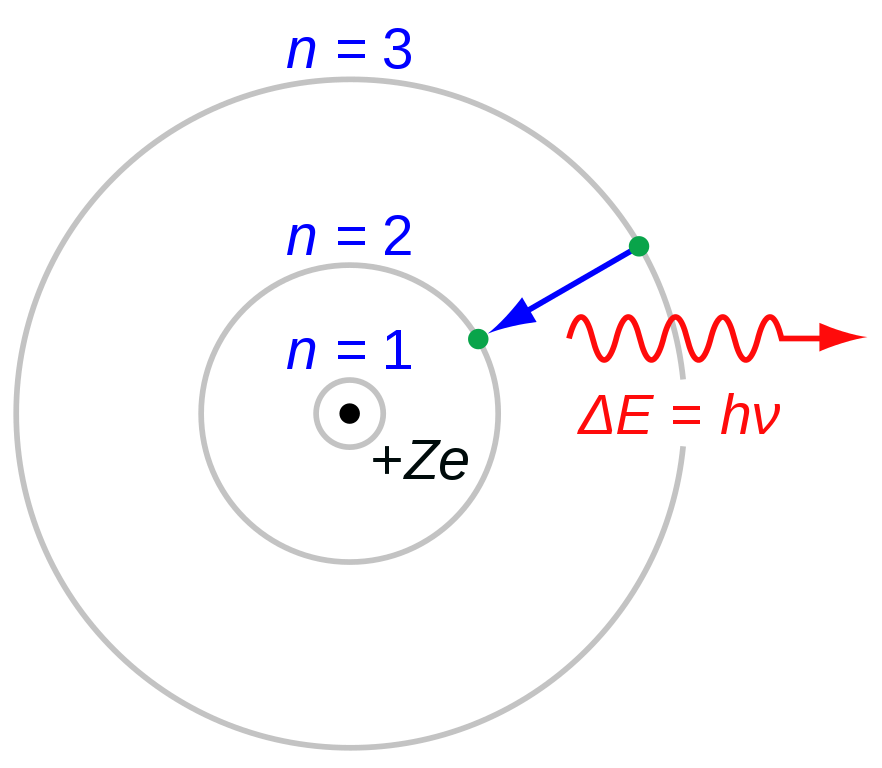
\includegraphics[width=0.33\linewidth]{Figures/bohr-atom-model} 

}

\caption{Illustration of bound-bound transition in the Bohr atomic model. Source: \href{https://commons.wikimedia.org/wiki/File:Bohr_atom_model.svg}{Wikipedia Commons}.}\label{fig:bohr-model}
\end{figure}

However, other predictions about the properties of the atom were wrong, and its implications were not observed in experiments. In the Schrödinger model, the electron of a one-electron atom, rather than travelling in fixed orbits around the nucleus, has a probability distribution allowing the electron to be at almost all locations in space, some being much more likely than others. Bohr theory (1913) was rejected in 1925 after the advent of quantum mechanics, but its model remains because despite its flaws and idealisations, \href{https://blogs.scientificamerican.com/guest-blog/why-it-s-okay-to-teach-wrong-ideas-in-physics/}{Bohr's model is useful for education}.

\hypertarget{the-models-of-benzene}{%
\subsection{The models of benzene}\label{the-models-of-benzene}}

\textbf{Models are as well purpose-dependent}. Suppose the next question. Which benzene model is better? A quantum mechanic model, or a structural formula?. On one side, the quantum mechanic model is more precise about the potential position of electrons. Additionally, is more similar to the target as it represents better its relevant properties. The structural model is simpler and easier to work with. In this case, theoretically tractable models such as structural models allow for functional group analysis in chemistry.



\begin{figure}[hbtp]

{\centering 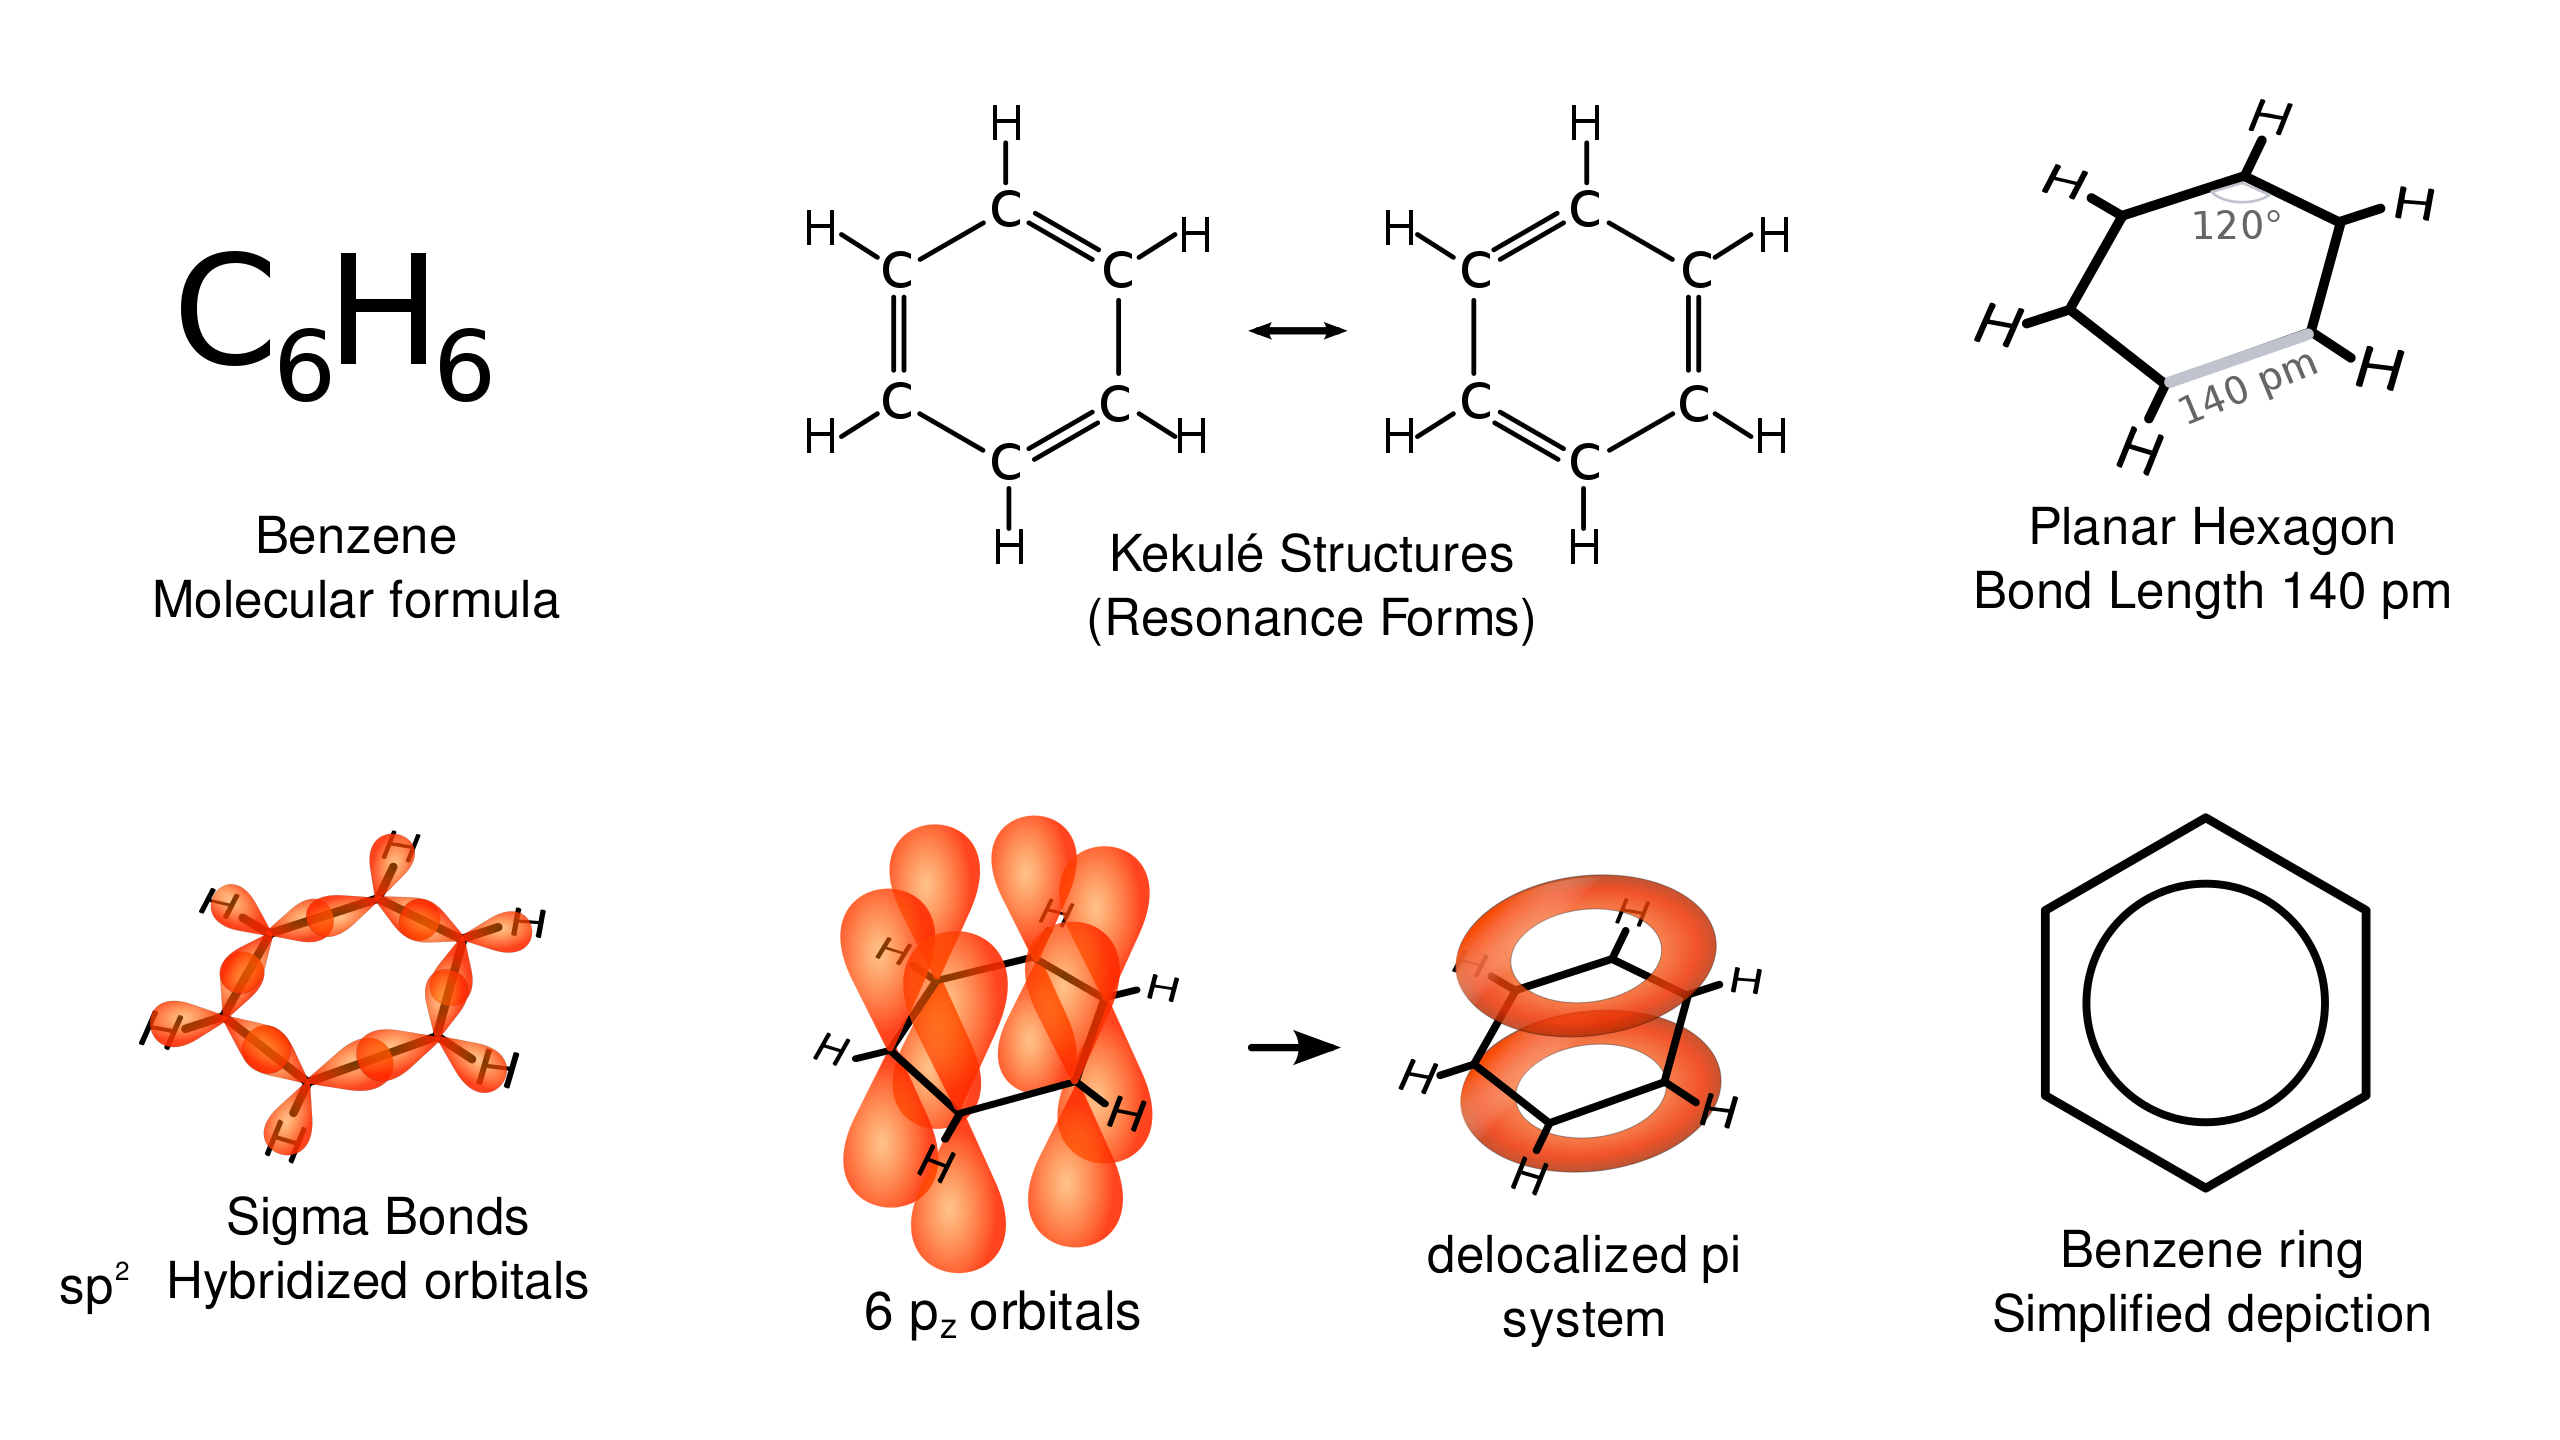
\includegraphics[width=0.9\linewidth]{Figures/Benzene_Representations} 

}

\caption{Various representations of Benzene. Source: \href{https://en.wikipedia.org/wiki/File:Benzene_Representations.svg}{Wikipedia Commons}.}\label{fig:benzene-model}
\end{figure}



\begin{figure}[hbtp]

{\centering 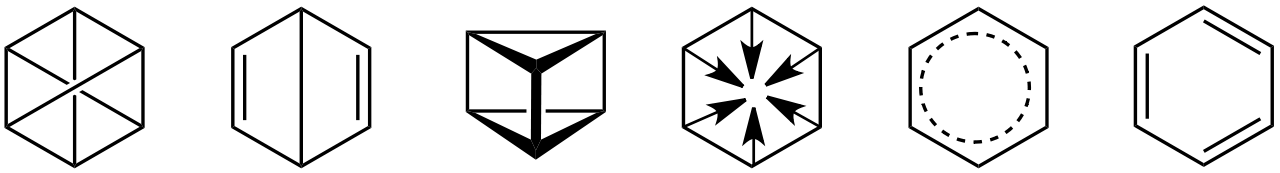
\includegraphics[width=0.9\linewidth]{Figures/Historic_Benzene_Formulae} 

}

\caption{Historic benzene structures (from left to right) by Claus (1867), Dewar (1867), Ladenburg (1869), Armstrong (1887), Thiele (1899) and Kekulé (1865). Dewar benzene and prismane are distinct molecules that have Dewar's and Ladenburg's structures. Thiele and Kekulé's structures are used today.}\label{fig:benzene-model-evolution}
\end{figure}

\hypertarget{models-as-analogies}{%
\subsection{Models as analogies}\label{models-as-analogies}}

\begin{wrapfigure}{R}{.36\textwidth}  
 \begin{center}
    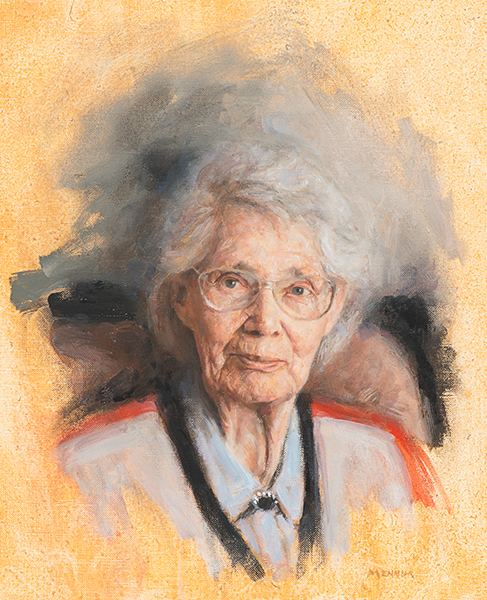
\includegraphics[width=.33\textwidth]{Figures/mary-hesse.jpeg}  
  \captionsetup{labelformat=empty}
  \caption{Prof. Mary Hesse (1924-2016), by Peter Mennim.} 
\end{center}
\end{wrapfigure}
\addtocounter{figure}{-1}

Philosopher Mary Hesse (1924-2016) argued that models act as analogies rather than descriptions of the targets. She distinguished between 3 kinds of analogies. In the first place, she considered that \textbf{positive analogies} hold between the aspects of a model and its target for which we have reasons to believe they are similar. An example of positive analogies can be found between mice and humans, which have similar hormone systems and physiology. On the other hand, the idealisations constitute \textbf{negative analogies}, such as the differences in size or lifespan between mice and humans. These negative analogies cover the properties in which model and target differ. Finally, \textbf{neutral analogies} concern the properties that we cannot investigate directly in the target, requiring the model for their study.

\begin{quote}
Without analogy there might be no knowledge: the perception of analogies is a first step towards classification and generalization. \citep{bunge2012method}
\end{quote}

For instance, the reaction to a certain drug or treatment of interest. At the initial stage, is not possible to tell whether the model-target relationships concerning these properties constitute positive or negative analogies because we do not know yet how the relevant target properties are affected. Instead, such properties are investigated in the model, and researchers hypothesise that the model is analogous to the target in such properties. For instance, we assume that the effects of a drug in mice will give us knowledge about its effects in humans.

\begin{quote}
The positive analogy between two items consists in the properties or relations they share (both gas molecules and billiard balls have mass); the negative analogy consists in the properties they do not share (billiard balls are colored, gas molecules are not); the neutral analogy comprises the properties of which it is not known (yet) whether they belong to the positive or the negative analogy (do billiard balls and molecules have the same cross section in scattering processes?). Neutral analogies play an important role in scientific research because they give rise to questions and suggest new hypotheses. --- \citep{sep-models-science}
\end{quote}

Consider again the Michelson and Morley experiment. Before the XX century, most physicists considered light as a wave. Their beliefs were justified on the many positive analogies between light, water and sound waves. For instance, light produces a diffraction pattern when encountering an obstacle, just as water and sound waves do. With this model in mind, physicists inferred a neutral analogy, namely, that light needs a medium to travel, as other waves require. They called this medium: luminiferous aether. The experiment from Michelson and Morley is a consequence of such model. However, the experiment revealed that such analogy was indeed a negative analogy, an idealisation. This discovery led people to replace the model of light for more precise models. Therefore, model manipulation allows discovering the effects of neutral analogies.



\begin{figure}

{\centering 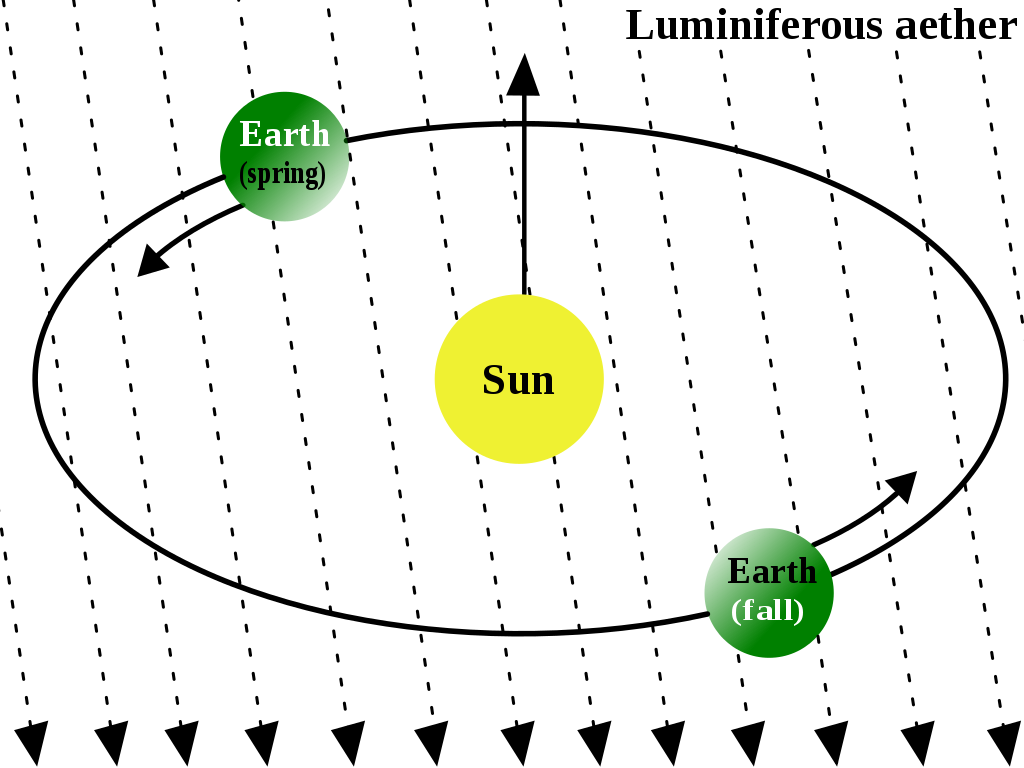
\includegraphics[width=0.5\linewidth]{Figures/luminiferous_aether} 

}

\caption{The luminiferous aether: it was hypothesised that the Earth moves through a "medium" of aether that carries light. Source: \href{https://commons.wikimedia.org/wiki/File:AetherWind.svg}{Wikipedia Commons}.}\label{fig:aether}
\end{figure}

\hypertarget{differences-between-models-and-experiments}{%
\subsection{Differences between Models and Experiments}\label{differences-between-models-and-experiments}}

There are several commonalities between models and experiments. Setting parameters and variables in models resembles experimental control. In the same way, model manipulation is akin to experimental manipulation. Moreover, model manipulation yields results that are observed, just as in experimental observations.

Notwithstanding, there are also important differences to bear in mind, which mainly concern the source of errors. For instance, the most troubling experimental errors concern internal validity questions, i.e.~the degree of confidence that the causal relationship put to test is not influenced by other factors or variables. For these reasons, researchers require careful design and control of experiments. Nonetheless, models are generally less sensitive to these issues since the modeller is aware of the idealisations and mechanisms of its models.

For modelling, the key concern is whether the relevant analogies between model and target hold. Such concern is usually not a problem for experiments, especially those conducted directly on the target. Once internal validity is assessed, researchers are confident that the inferences drawn from the experiment refer to the target. However, inferences drawn from model manipulation constitute neutral analogies considered as hypotheses regarding the target, requiring further testing and justification. This last step is error-prone.

\hypertarget{what-makes-a-good-model}{%
\subsection{What makes a good model?}\label{what-makes-a-good-model}}

Since models are purpose dependent, there is no exhaustive set of sufficient and necessary conditions to define what a good model is. Nonetheless, there are some common criteria (e.g.~robustness, simplicity, tractability) that can be balanced, but is often impossible to optimise all criteria at the same because some criteria are complements of each other.

The \textbf{similarity} criterion can for example assess physical resemblance. More generally, we could say that a model \(M\) is similar to target \(X\) if and only if \(M\) is similar to \(X\) with respect to the set of properties \(P\) to a certain degree. However, this definition does not tell us which properties should be optimised. For instance, for a scale model of an air plane aimed at aerodynamic studies, it might be more justified to maximise the similarities of geometric properties over the interior design (e.g.~the number of seats might not be relevant since the cabin is closed). Therefore, the purpose of the model justifies maximising one set of properties over another, in particular, the properties that are relevant for the research purpose.

\textbf{Robustness} expresses how model results are affected by condition changes. Therefore, a model result is robust (w.r.t. some condition) if changing such condition does not alter the result. For example, all properties except one (e.g.~plane hull colour) can be kept fixed to test whether painting the plane with a different colour might affect its aerodynamic properties. If the result remains equal, we can say the model is robust with respect to the hull colour. Perhaps such property is not relevant to the research purpose, but that is not enough to justify removing the property.



\begin{figure}

{\centering 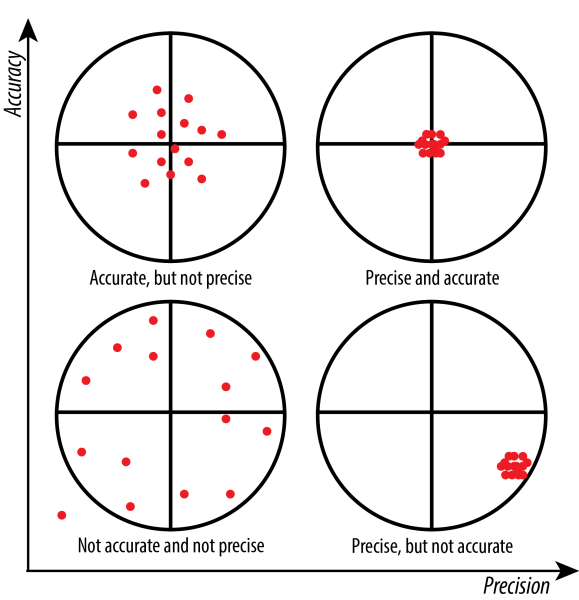
\includegraphics[width=0.66\linewidth]{Figures/prec_vs_acc} 

}

\caption{Accuracy consists of trueness (proximity of measurement results to the true value) and precision (repeatability or reproducibility of the measurement). Source: \href{https://wp.stolaf.edu/it/gis-precision-accuracy/}{St.~Olaf College}.}\label{fig:prec-vs-acc}
\end{figure}

Another model criterion to consider is \textbf{precision} (w.r.t. parameters). We say that model \(M_1\) is more precise than \(M_2\) if the parameter specifications of \(M_1\) \emph{imply} those from \(M_2\). This definition is better understood through an example. Consider the following models \(M_1\), \(M_2\), and \(M_3\) and below definitions. The first model describes a rate of changes as a function of \(X\). \(M_2\) is more precise as describes the rate of changes as a linear function of \(X\). The description of \(M_2\) implies the description of \(M_1\). Linear functions of \(X\) are a subset of functions of \(X\). Finally, the third model is yet more precise as it indicates an absolute value of the parameter \(a\), reducing the subset of linear functions from the definition of \(M_2\) to a particular linear function. Importantly, parameter precision is a property of the model alone, not of the relationship between model and target. Although precision offers potential for high accuracy, it is no warrant for it. For instance, if the actual rate of linear change would be other than \(1.2X\), then the less precise model \(M_2\) would be more accurate than \(M_3\). Similarly, if the rate of change would not change linearly, the more general model \(M_1\) would be more accurate than the alternatives.

\begin{itemize}
\tightlist
\item
  \(M_1: dX/dt = f(X)\)
\item
  \(M_2: dX/dt = aX\)
\item
  \(M_3: dX/dt = 1.2X\)
\end{itemize}

\begin{tipbox}

\textbf{Note for data scientists!}

Questions regarding scientific models also concern Machine Learning models to a great extent. For example, consider the precision and accuracy criteria. The following paragraph is extracted from \href{https://dl.acm.org/doi/pdf/10.1145/2347736.2347755}{the article ``A Few Useful Things to Know About Machine Learning'' by Pedro Domingos}.

\begin{quote}
Everyone in machine learning knows about overfitting, but it comes in many forms that are not immediately obvious. One way to understand overfitting is by decomposing generalization error into bias and variance. Bias is a learner's tendency to consistently learn the same wrong thing. Variance is the tendency to learn random things irrespective of the real signal. Figure illustrates this by an analogy with throwing darts at a board. A linear learner has high bias, because when the frontier between two classes is not a hyperplane the learner is unable to induce it. Decision trees do not have this problem because they can represent any Boolean function, but on the other hand they can suffer from high variance: decision trees learned on different training sets generated by the same phenomenon are often very different, when in fact they should be the same. Similar reasoning applies to the choice of optimization method: beam search has lower bias than greedy search, but higher variance, because it tries more hypotheses. Thus, contrary to intuition, a more powerful learner is not necessarily better than a less powerful one. --- \citep{domingos2012few}
\end{quote}

\end{tipbox}

\textbf{Simplicity} is often another criteria that affects models. A simpler model might fit very well its purpose. For example, underground maps often misrepresent distances or omit unnecessary details such as roads, monuments, etc. Such simplification is suited for the particular purpose of travelling in the underground but is not useful for other purposes. We can say a model is simpler if it contains less parameters, considers less variables and uses less operations than another model. Therefore, simplicity is a virtue with respect to the models and not to targets. Is usually a practical criterion that facilitates the model use.

Related to simplicity, we can find \textbf{tractability}. We say a model is tractable (w.r.t. a set of rules) if the relevant model result may be obtained by applying certain principles to the model. For instance, models solved through analytical methods (e.g.~mathematical proofs) are called analytically tractable in contrast to models for which results can only be approximated through numerical simulations methods. Tractability implies the existence of methods to analyse and solve such models. In this sense, \textbf{theoretical tractability} considers theoretical principles to assess the suitability of the model for certain operations. For instance, a structural representation of a chemical compound allows for the application of functional group classification (this is an example of theoretical principle to fulfil). In contrast, a quantum mechanical model is more accurate but does not allow for such operation. Therefore we consider it a less tractable model.

Finally, \textbf{transparency} is an epistemic value that assesses the degree to which the model user can cognitively understand how the model result is produced. This criterion is known in artificial intelligence as interpretability and/or explainability. For example, a decision tree is often human-readable while the nature of neural networks creates obfuscated models difficult to interpret. Transparent models allow to back-track the result and understand how it was produced from a given input. A transparent model enables the scientist to check the correctness of the results, which is especially important when employing models developed by third parties.

Again, most of the previous virtues will require certain trade-off. Increasing an epistemic value often entails decreasing another one. Therefore, building or choosing a model requires finding the best trade-off for the model's purpose.

\hypertarget{models-as-mirrors}{%
\subsection{Models as mirrors}\label{models-as-mirrors}}

A common way to consider models is as mirrors of the real world. Very often, models are built to be as similar as possible to the target. This is common in highly complex projects such as brain simulations of the neural networks that represent human brain activity or epidemic simulations in which all the available demographic information (e.g.~transportation, habits) is considered. The aim of such complex projects is to build a model as a replacement of the actual target system. In the case of epidemic simulations, it is clear that is not feasible to conduct real-world experiments, but the simulation can serve as a way to try different vaccination strategies that might, for instance, prioritise the vaccination of potential super spreaders, i.e.~people who are in contact with many people during their daily routine (e.g.~supermarket cashiers, waiters). In this sense, we say that the simulation is \emph{mirroring} the world. Another example from engineering includes finite element analysis (FEA) which is used to divide a complex problem into smaller elements to facilitate calculations.

This type of model is very similar to the target and require high precision modelling. However, these advantages come at a cost. For instance, they compromise the simplicity, transparency and sometimes the tractability of the models. Despite the high similarity of the models to their target systems, it is not enough to avoid external validity issues. For example, FEA employs a mesh consisting of millions of small elements that mould the physical shape of the analysed structure. Then, calculations are made for each element. Such approximations are usually polynomial, which means that the structural elements have been interpolated, and their precision is bounded to the mesh size. Therefore, the accuracy depends on the purpose of the analysis (e.g.~car, hardware tools, camera).

\begin{figure}

{\centering 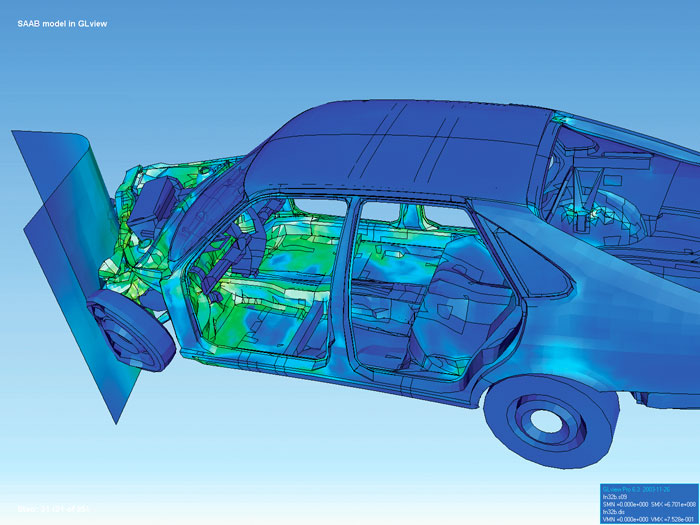
\includegraphics[width=0.5\linewidth]{Figures/FAE_visualization} 

}

\caption{A visualization of an asymmetrical collision analysis using the finite element analysis method.}\label{fig:fea}
\end{figure}

\hypertarget{models-as-isolations}{%
\subsection{Models as isolations}\label{models-as-isolations}}

An alternative perspective is to consider models as isolations of particular features of the complex world. This consideration is motivated by the following question. Can models be similar to their target systems and still be simple? We have previously seen that these two factors are very often inversely related. Isolated models choose a particular aspect of the target, disregarding all the rest. Then, a model is built to represent the behaviour of such factors as accurately as possible.

\begin{figure}

{\centering 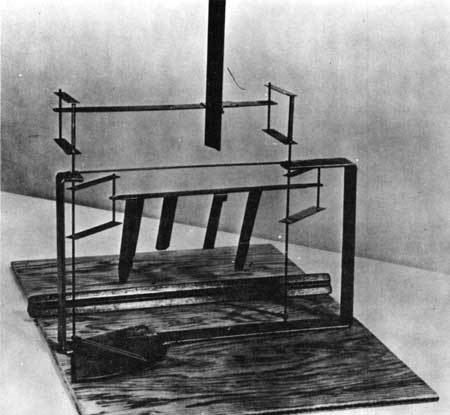
\includegraphics[width=0.5\linewidth]{Figures/lift} 

}

\caption{Reproduction of lift balance used in 1901 wind tunnel; model airfoil in testing position. Source: NPS.}\label{fig:lift}
\end{figure}

During the development of the airplane. George Cayley (1773 - 1857) proposed to separate the airplane system into 3 subsystems: Lift, Propulsion, Control. After this, the problem is divided into three problems, i.e.~how to obtain lift, how to provide propulsion, and how to offer control. The Wright Brothers developed a separate model for each of this subsystems. As can be observed in Figure \ref{fig:lift}, the lift balance model does not resemble an airplane. Similarly, their propeller model was not attached to the airplane. Likewise, they employed gliders to test their control systems. This contrast with the approach of other inventors, such as Hiram Maxim, who attempted to build a full scale from scratch.
An overview of the Wright Brothers Invention Process can be found at \href{https://wright.nasa.gov/overview.htm}{NASA's website}.



\begin{figure}[h]

{\centering 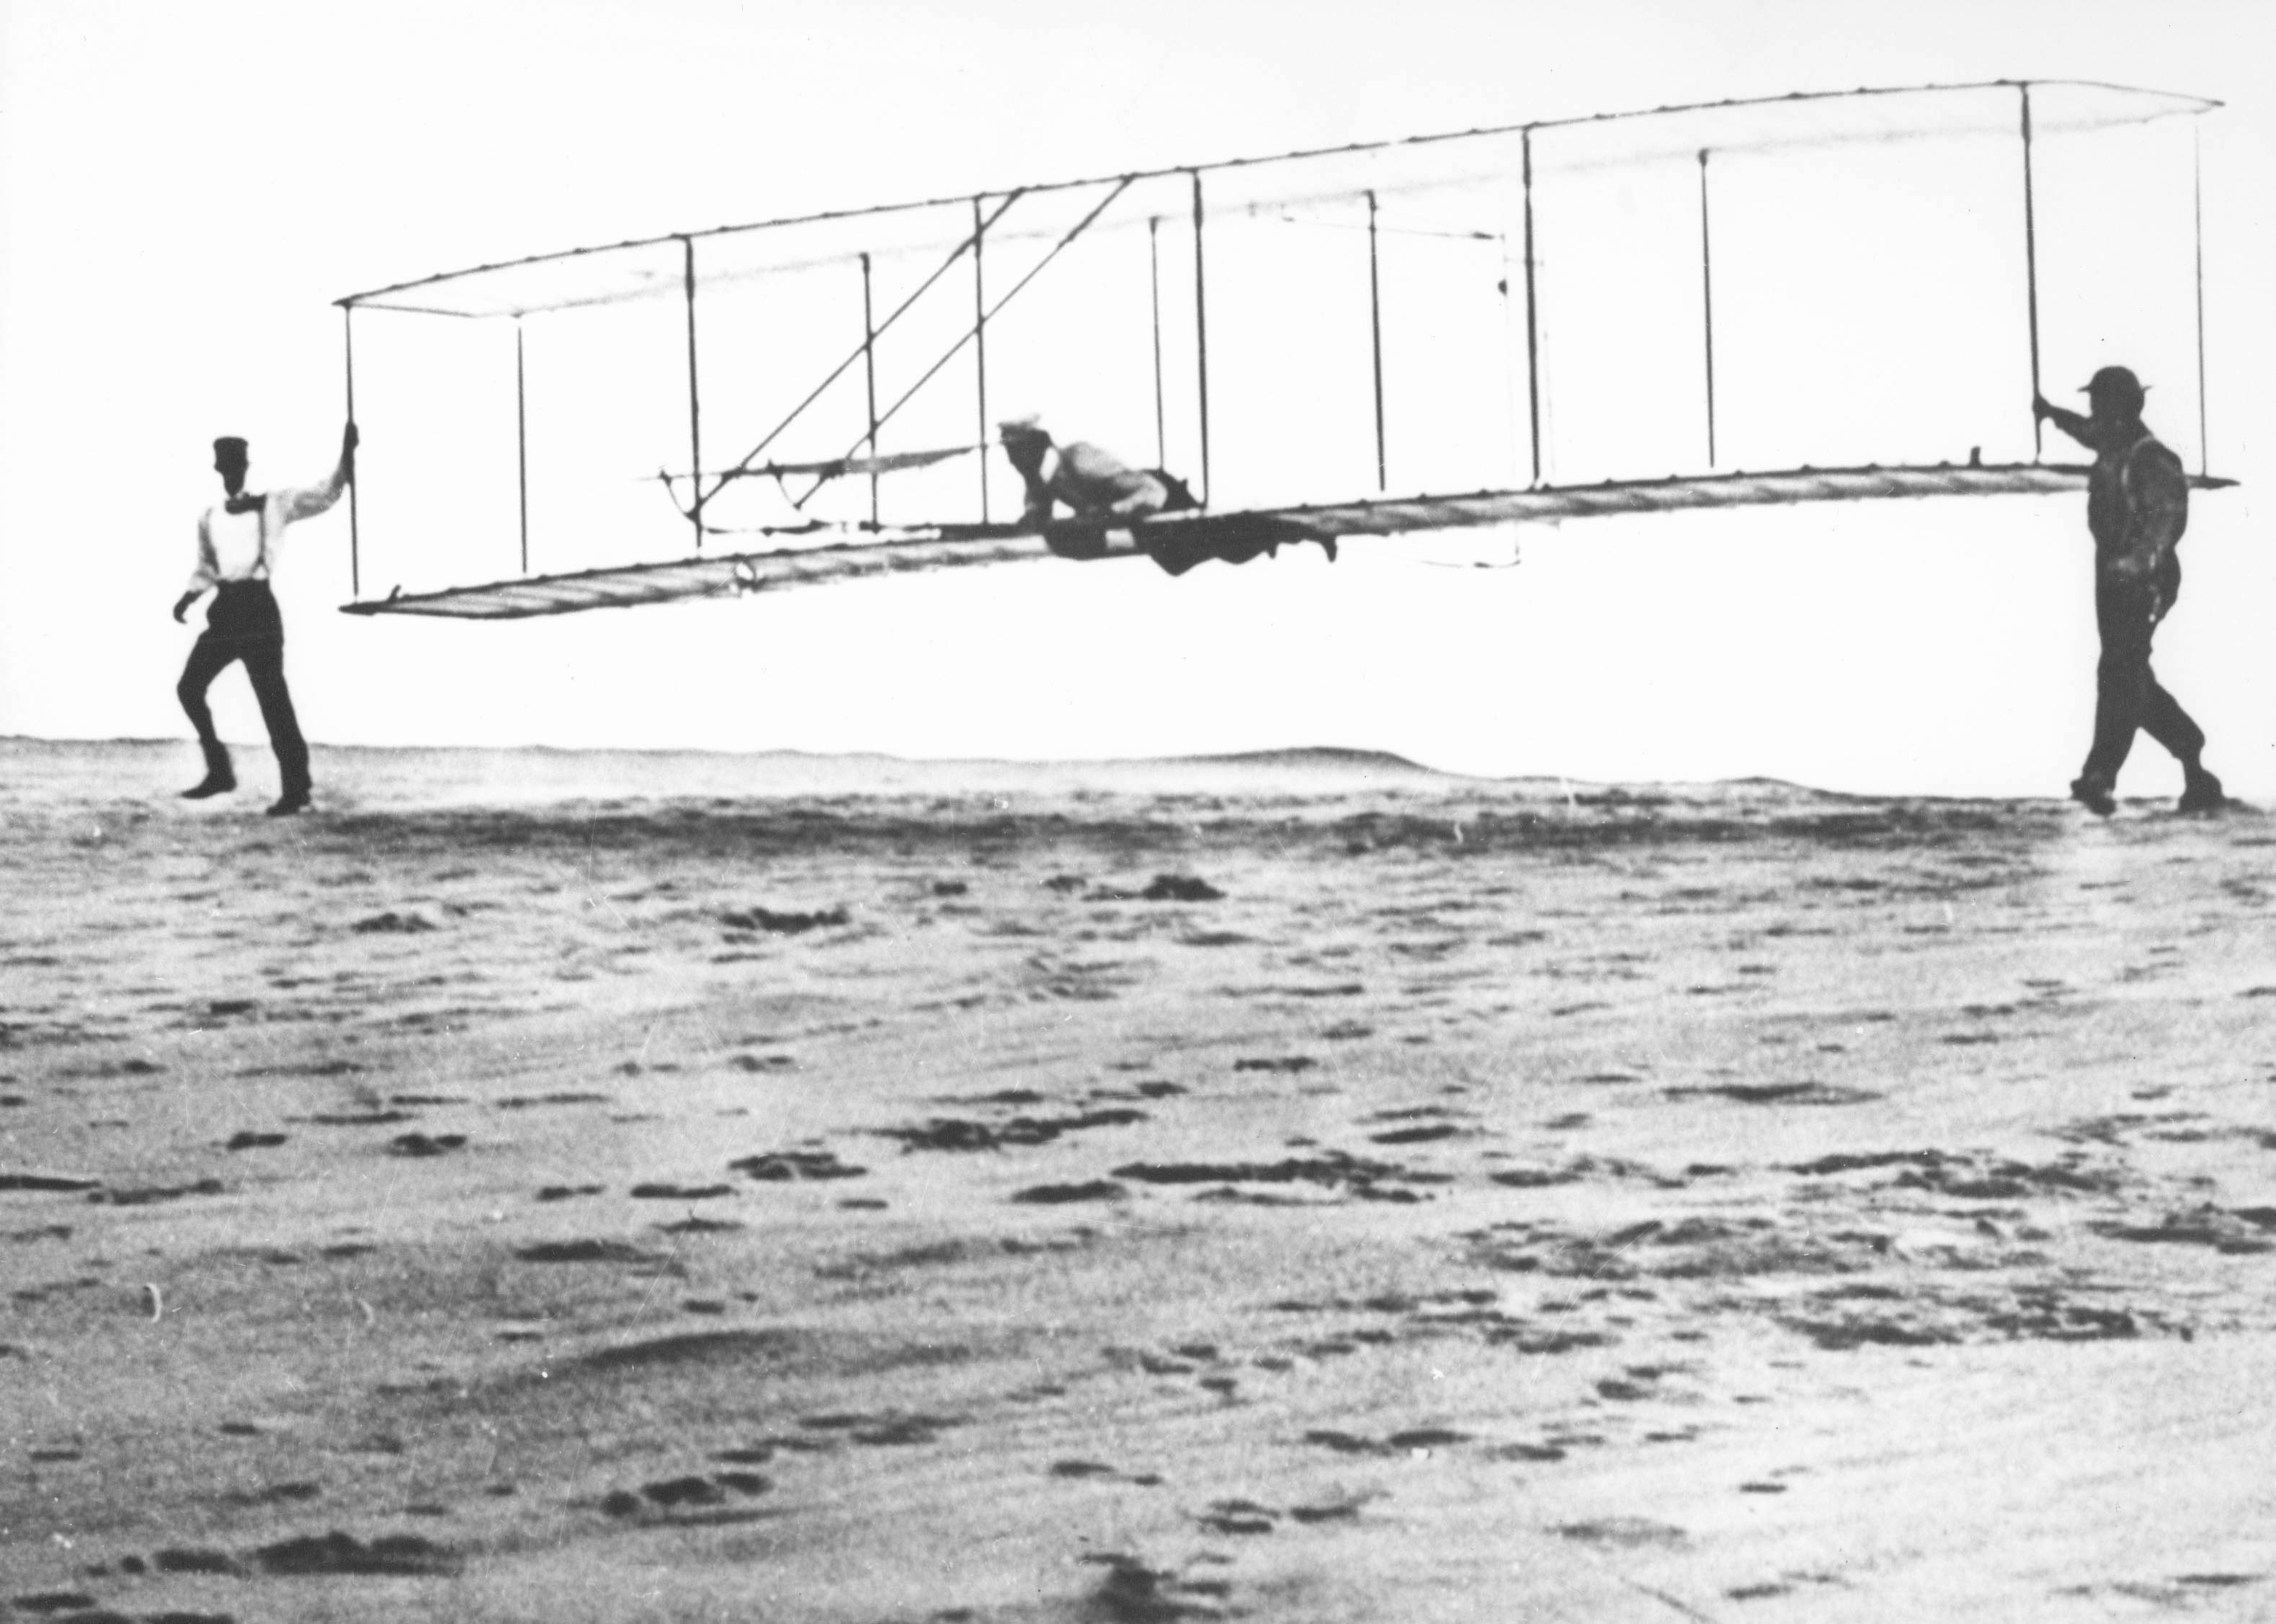
\includegraphics[width=0.5\linewidth]{Figures/Wright_Brothers} 

}

\caption{Historic photo of the Wright brothers' third test glider being launched at Kill Devil Hills, North Carolina, on October 10, 1902. Wilbur Wright is at the controls, Orville Wright is at left, and Dan Tate (a local resident and friend of the Wright brothers) is at right.}\label{fig:brothers}
\end{figure}

However, a limitation of this approach is that the target system must be dividable in different subsystems. Similarly, the results of valid isolating models might not look like the real world phenomena simply because the latter is a combination of effects. On the other side, the model represents a single effect in isolation. Therefore, the validation of isolated models is problematic.

\hypertarget{examples-2}{%
\section{Examples}\label{examples-2}}

\hypertarget{willow}{%
\subsection{Willow tree experiment}\label{willow}}

\begin{wrapfigure}{R}{.25\textwidth}  
 \begin{center}
    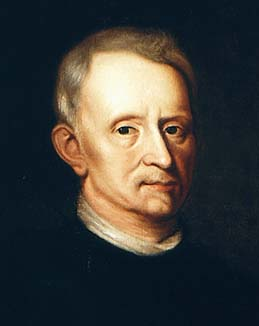
\includegraphics[width=.22\textwidth]{Figures/Jan_Baptist_van_Helmont_portrait.jpg}  
  \captionsetup{labelformat=empty}
  \caption{Portrait of Jan Baptist van Helmont by Mary Beale, c.1674.} 
\end{center}
\end{wrapfigure}
\addtocounter{figure}{-1}

Jan Baptist van Helmont (1580 - 1644) was a chemist, physiologist, and physician from the Spanish Netherlands (current Belgium).
In 1634, Jan Baptist was arrested by agents of the Spanish Inquisition for the crime of studying plants and other natural phenomena. During his house arrest, he studied how plants grew. The prevailing theory at the time, stated that plants grew by eating soil, and Jan Baptist conceived an experiment to test this idea. Such prevailing theory has its origins in the ancient Greeks.

Jan Baptist started by weighing a small willow tree (2.28 kg) and then weighed the dry soil (90 kg) in which he planted the tree. To prevent the dust from the surrounding air from mixing with the earth, the rim of the pot was protected, covered with a sheet of iron covered with tin and pierced by many holes. The tree was watered with rainwater or (when necessary) with distilled water. Jan Baptist left the tree for five years. After the five years had passed, Jan Baptist re-weighed the tree, which weighed 169 pounds (about 77 kg). He also re-weighed the dried soil and found the same 200 pounds (90 kg) minus about 2 ounces (56 gm).

He wrongly concluded that the mass gain of the tree was produced by the water, which was his only intervention on the system. Although the experiment was carefully conducted, the conclusions derived from the experiment were wrong because the theory on which it was based was incorrect. Importantly, the fact that Helmont used soil contradicted his hypothesis that only water was needed for plant growth \citep{hershey1991digging}.

Jan Baptist did not know anything about photosynthesis. During the photosynthesis, carbon from the air and minerals from the soil are used to generate new plant tissue. Ironically, Helmont has been credited with discovering carbon dioxide \citep{hershey1991digging}.

The employment of the balance during van Helmont's experiment was an important improvement; Jan Baptist believed that the mass of materials had to be accounted for during the study of chemical processes. This experiment is considered the first quantitative experiment in plant nutrition. It is also a great example of how firm conclusions can be misled by lack of knowledge of the studied system. Jan Baptist failed to control for an important background factor.



\begin{figure}[H]

{\centering 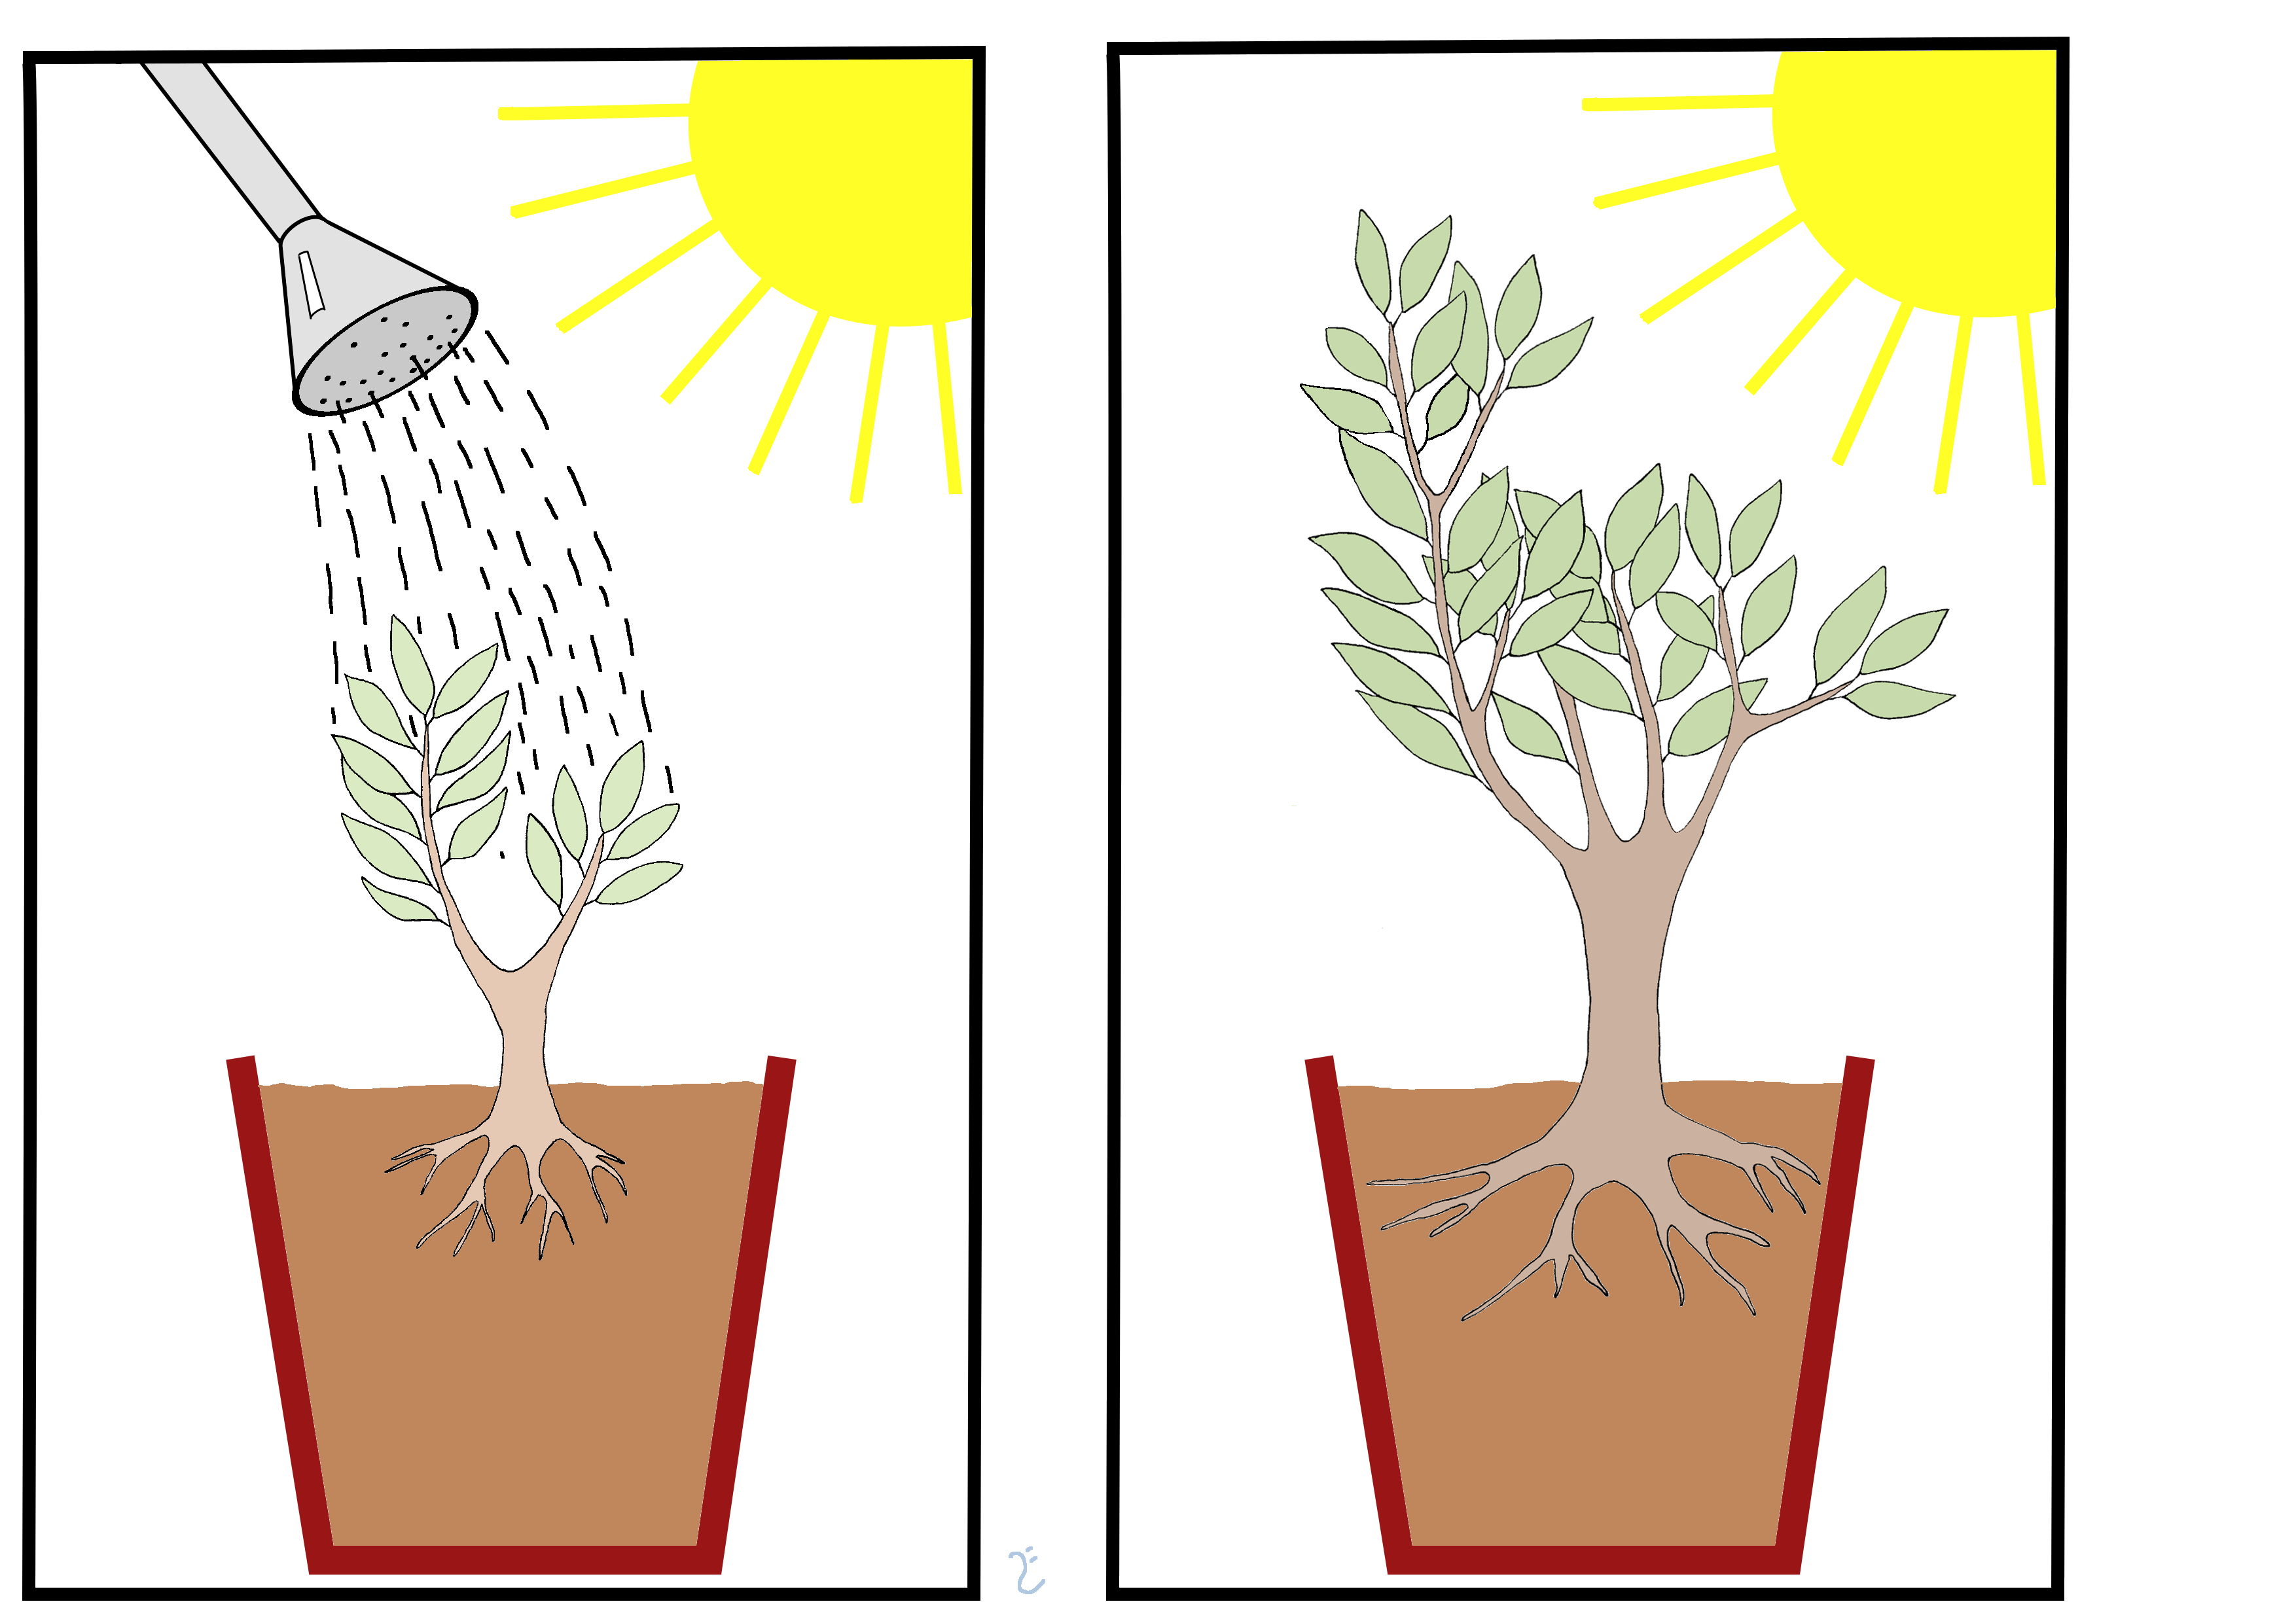
\includegraphics[width=0.7\linewidth]{Figures/Van_Helmont_Experiment} 

}

\caption{Illustration of the willow tree experiment. By \href{https://commons.wikimedia.org/wiki/File:Van_Helmont_Experiment.jpg}{Lars Ebbersmeyer}.}\label{fig:van-helmont}
\end{figure}

\hypertarget{john-snow}{%
\subsection{1854 Broad Street cholera outbreak}\label{john-snow}}

\begin{wrapfigure}{R}{.25\textwidth}  
 \begin{center}
    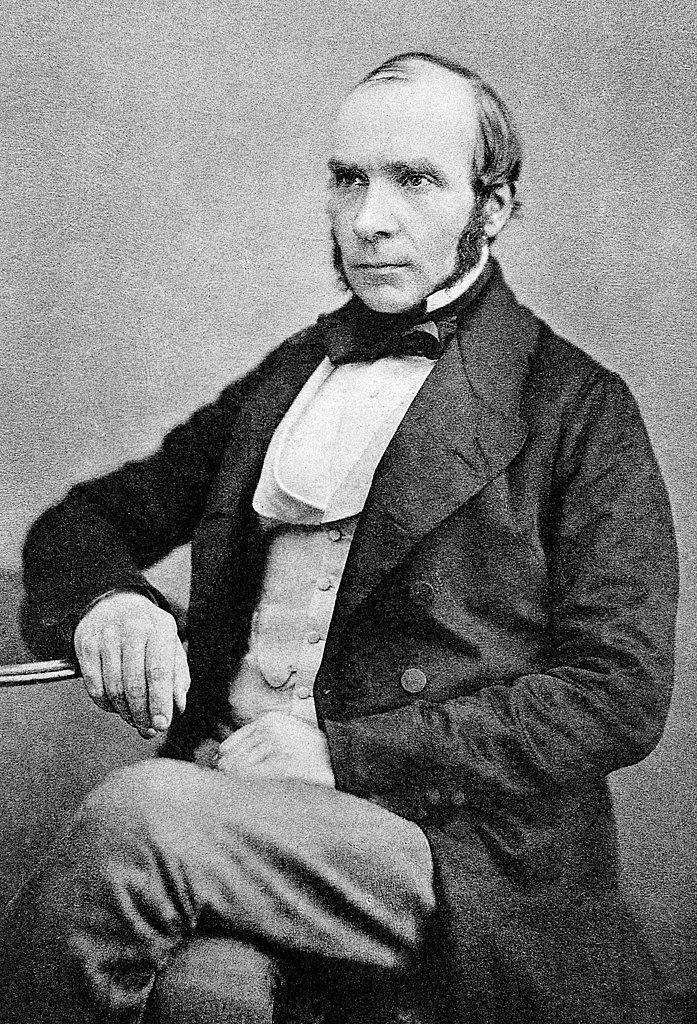
\includegraphics[width=.22\textwidth]{Figures/John_Snow.jpg}  
  \captionsetup{labelformat=empty}
  \caption{Dr. John Snow (1813-1858), British physician.} 
\end{center}
\end{wrapfigure}
\addtocounter{figure}{-1}

The birth of epidemiology and public health is often attributed to the Natural Experiment described by Dr.~John Snow in the mid-1800s when he investigated the relationship between drinking contaminated water and the incidence of cholera \citep{applied_stats_healthcare}. The case of Dr.~Snow is very popular in public health science and can be found in several books and posts on-line but I recommend the explanation given in Chapter 7 from The Book of Why \citep{book-of-why} as the authors also re-formulate the case in causal terms, using concepts that were not available in the mid-1800s. Below, I give a summarised account of this study.

\begin{quote}
\emph{Miasma}: ``A vaporous exhalation formerly believed to cause disease.''
\end{quote}

Since the 1830s, various epidemics spread across Europe but were often attributed to social unrest and political upheaval. During the 1850s, there were several theories and misconceptions about the causes of cholera outbreaks. The miasma theory attempted to explain outbreaks of bubonic plague and cholera, stating that they were caused by a form of ``bad air''. According to the competing theory, i.e.~the germ theory of disease, the cause of the outbreak was a yet unknown germ. However, in 1853, disease-causing germs had not yet been observed under a microscope and the germ theory of disease was not established yet. Louis Pasteur did not demonstrate the relationship between germ and disease until the 1860s. Therefore, the prevailing theory was that a miasma of unhealthy air caused cholera.

In August 1854, a major outbreak of cholera occurred in Soho, London (United Kingdom). In just three days, 127 people died in Broad Street. By September, 500 people had died. John Snow was skeptical of the prevailing miasma theory and theorized that the cause was the presence of an agent in the contaminated water source from certain water supplying companies \citep{applied_stats_healthcare}. Namely, the Southwark and Vauxhall Company and the Lambeth Waterworks Company. The main difference between the two companies was that the former drew its water from London Bridge, which was downstream from London's sewers. Years earlier, Lambeth had moved its water intake so that it would be upstream of the sewers.



\begin{figure}

{\centering 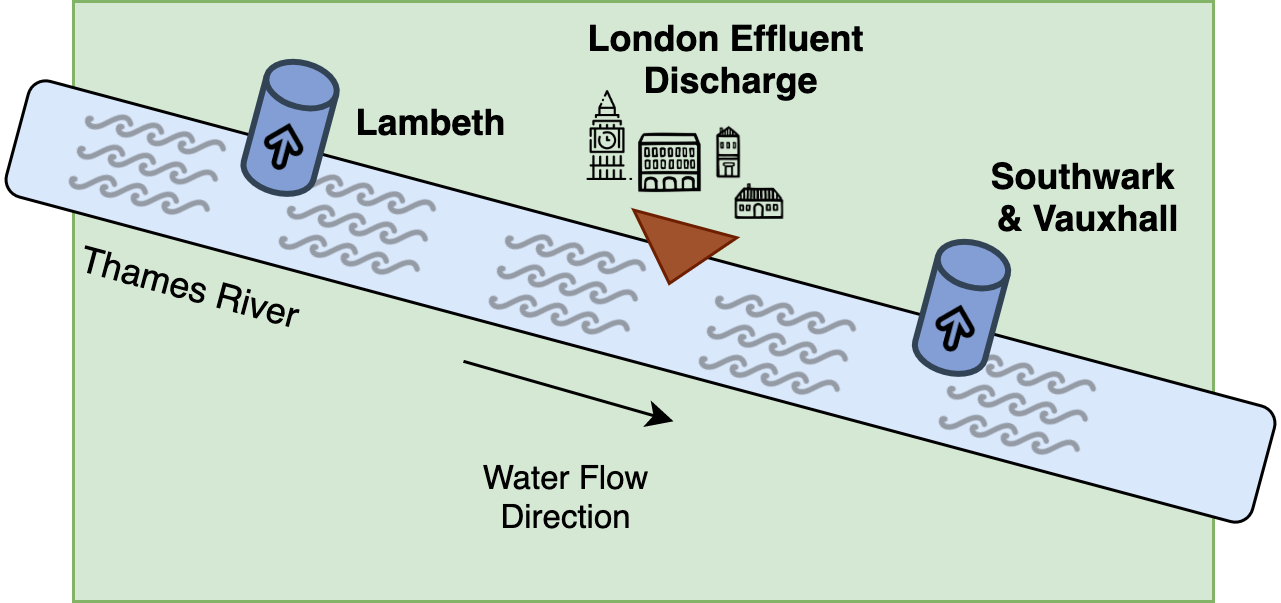
\includegraphics[width=0.66\linewidth]{Figures/JohnSnowRiver} 

}

\caption{Water distribution by the Lambeth Water and the Southwark \& Vauxhall Companies.}\label{fig:thames}
\end{figure}

Therefore, the customers of the Southwark and Vauxhall Company were getting water contaminated by the excrements of cholera victims, whereas Lambeth users were drinking uncontaminated water.

In consequence, districts supplied by the Southwark and Vauxhall Company had a death rate eight times higher than other districts. At this point, the evidence supporting the hypothesis of water contamination is just circumstantial. The causal diagram from Figure \ref{fig:snow-dia-A} depicts the situation. A proponent of the miasma theory could argue that the effect of miasma was strongest in those districts \citep{book-of-why}.

\begin{figure}

{\centering 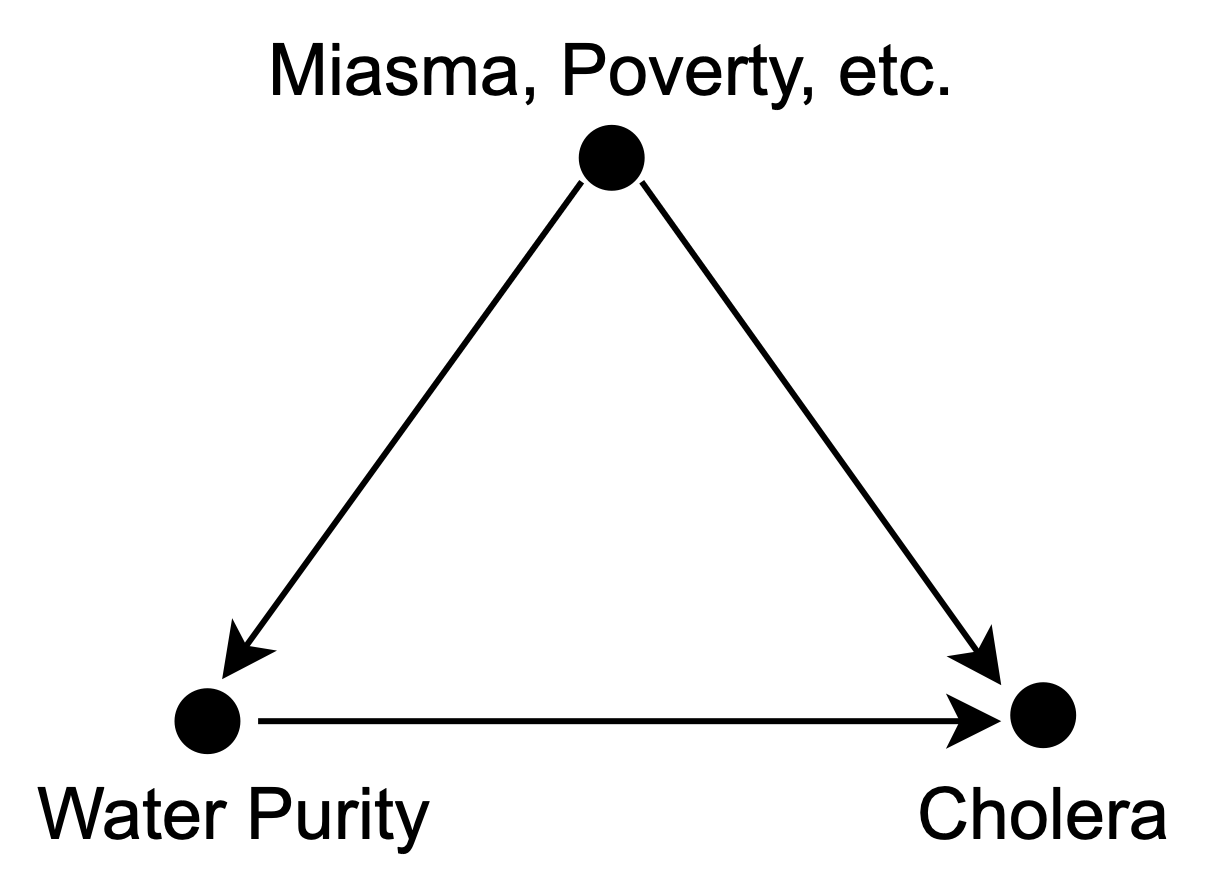
\includegraphics[width=0.33\linewidth]{Figures/SnowDiagramA} 

}

\caption{Causal diagram for cholera for the case of John Snow.}\label{fig:snow-dia-A}
\end{figure}

Then, Snow noted that in some districts water was served by both companies (see Fig. \ref{fig:snow-map}), and even there, the death rate was still higher in the houses where water was supplied by the Southwark and Vauxhall Company. Those households did not showcase any difference in terms of poverty or miasma. Snow wrote: ``each company supplies to both rich and poor, both large houses and small; there is no difference either in the condition or occupation of the persons receiving the water of the different companies.'' \citep{book-of-why}.

\begin{longtable}[]{@{}lc@{}}
\caption{Relation of the household water source and deaths}\tabularnewline
\toprule
Source of water & Deaths \\
\midrule
\endfirsthead
\toprule
Source of water & Deaths \\
\midrule
\endhead
Southwark and Vauxhall company & 286 \\
Lambeth company & 14 \\
Direct from the river & 22 \\
Pump wells & 4 \\
Ditches & 4 \\
Unknown & 4 \\
\bottomrule
\end{longtable}

\textbf{It is precisely at this point where the natural experiment takes all its strength.} Around 300 people of both sexes, every age, and socio-economic class were naturally divided into two groups without them to know. One group received pure water, whereas the other received water mixed with sewage.

The observations of John Snow introduced a new variable into the causal diagram (see Fig. \ref{fig:snow-dia-B}), the \textbf{Water Company}. In this new diagram we can see that there is no arrow between Miasma and Water Company, therefore both variables are independent. Moreover, we can note the presence of an arrow between Water Company and Water Purity. Finally, the diagram depicts a third assumption. There is no direct arrow from Water Company to Cholera, i.e.~water companies do not deliver cholera to their customers in any other way.

\begin{figure}[htb]

{\centering 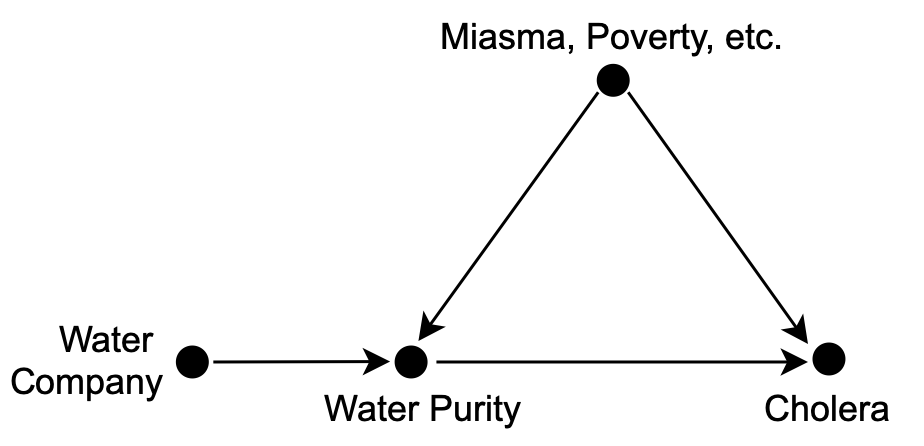
\includegraphics[width=0.5\linewidth]{Figures/SnowDiagramB} 

}

\caption{Causal diagram after the introduction of an instrumental variable.}\label{fig:snow-dia-B}
\end{figure}

A variable that satisfies these properties is called an \textbf{instrumental variable}. See \citep{pokropek2016introduction} for examples of valid and invalid instrumental variables and \href{https://scpoecon.github.io/ScPoEconometrics/IV.html}{SciencesPo} for econometric examples. \textbf{Since there are no confounders of the relation between Water Company and Cholera, any observed association must be causal}. Similarly, the association between Water Purity and Cholera is also causal.

\begin{quote}
Specifically, an instrumental variable Z is an additional variable used to estimate the causal effect of variable X on Y. The traditional definition qualifies a variable Z as an instrumental (relative to the pair (X, Y)) if (i) Z is independent of all variables (including error terms) that have an influence on Y that is not mediated by X and (ii) Z is not independent of X. --- \citep{pearl2000causality}
\end{quote}

Although today miasma theory has been discredited, poverty and location are clear confounders. In \citep{book-of-why}, the authors show how instrumental variables can be used to determine the number of lives that could have been saved by purifying the water supply. The instrumental variable \textbf{Water Company} allow us to find the effect of \textbf{Water Purity} on \textbf{Cholera} even without being able to control, or collect data on, the confounder variables (poverty, location, etc.).

One of the main innovations of John Snow approach was to focus on death rates in districts served by two water companies rather than on data from victims of the Broad Street pump which drew water from a well.

\begin{quote}
A transitional period began in the late 1850s with the work of Louis Pasteur. This work was later extended by Robert Koch in the 1880s. By the end of that decade, the miasma theory was struggling to compete with the germ theory of disease. Viruses were initially discovered in the 1890s. Eventually, a ``golden era'' of bacteriology ensued, during which the germ theory quickly led to the identification of the actual organisms that cause many diseases. --- Wikipedia, \href{https://en.wikipedia.org/wiki/Germ_theory_of_disease}{Germ theory of disease}.
\end{quote}

\begin{figure}[htbp]

{\centering 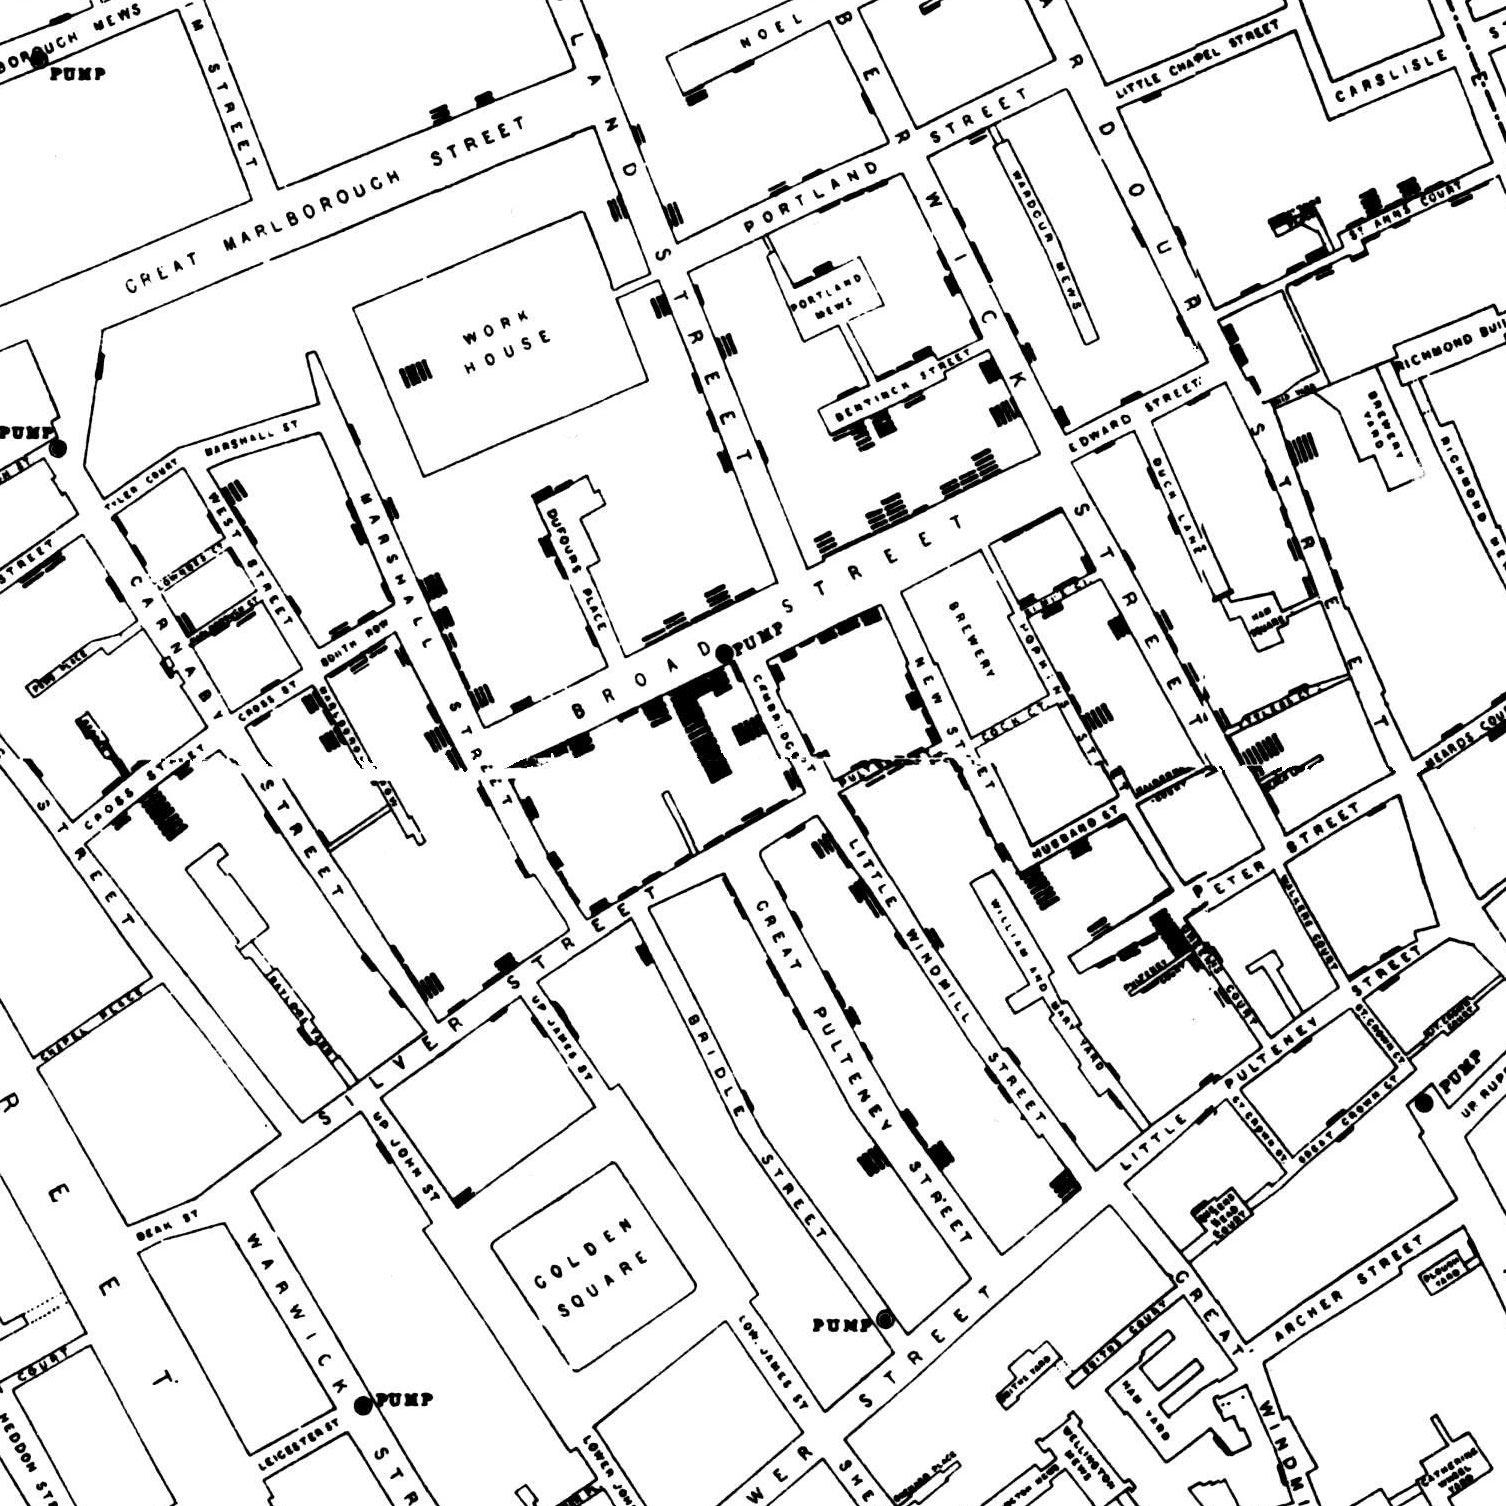
\includegraphics[width=1\linewidth]{Figures/snow-cholera-map-crop} 

}

\caption{Detail of John Snow’s map of Cholera in the Broad Street outbreak in 1854. Each bar represents one death in a topography that attempted to relate the water source (“Pump”) to pattern of cases in the neighborhood outbreak.}\label{fig:snow-map}
\end{figure}

\hypertarget{stats-abuse}{%
\chapter{Experimental Control and Statistical Abuse}\label{stats-abuse}}

\begin{notebox}

\begin{center}
\textbf{Course Note:}

\end{center}

This chapter is under construction. Some content is hidden.

\end{notebox}

\hypertarget{stats-overview}{%
\section{Overview}\label{stats-overview}}

Daniel did not think of everything when designing his experiment. He did not take confounding bias into account. For instance, Daniel and his friends could have been healthier than the control group. Under such supposition, their strong appearance after ten days of a vegetarian diet may have nothing to do with the diet itself. Perhaps, they would have become even stronger if they had eaten the meat from the king. As we have seen in previous examples presented in this book, confounding bias happens when a variable influences both who is chosen for the treatment group as well as the experiment outcome. These variables might be known variables or act as a lurking third variable we are not aware of. Such variables are easy to spot in causal diagrams.

The term \emph{``confounding''} means \emph{``to pour, mingle, or mix together''}, and Figure \ref{fig:confounder-simple} illustrates why such name was chosen to denominate these situations. The true causal effect \(X -> Y\) is \emph{mixed} with the spurious correlation between \(X\) and \(Y\) induced by the fork \(X <- Z -> Y\) \citep{book-of-why}.

\begin{figure}

{\centering 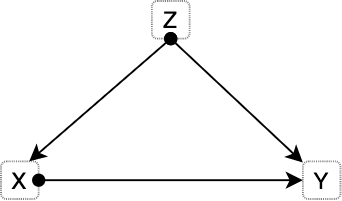
\includegraphics[width=0.33\linewidth]{Figures/causal_diagram_confounder_simple} 

}

\caption{Most basic version of confounding situation: Z is a confounder of the proposed causal relationship between X and Y.}\label{fig:confounder-simple}
\end{figure}

\hypertarget{the-smoke-debate---part-ii}{%
\subsection{The smoke debate - Part II}\label{the-smoke-debate---part-ii}}

Many famous cases present these confounding situations. For instance, this book previously tackled the debate around smoking and lung cancer. Austin B. Hill and Richard Doll noticed that hidden biases could be present in their previous case-control studies, and the replication of the studies would not be enough to overcome them. In consequence, they began a prospective study (1951) in which they considered 60.000 physicians from United Kingdom consisting of questionnaires tackling their smoking habits. These physicians were followed over time. In just five years, heavy smokers showed a death rate from lung cancer 24 times higher than non-smokers. A similar study conducted in the United States showed that smokers died from lung cancer 29 times more often than non-smokers while heavy smokers died 90 times more frequently. However, former smokers reduced their risk by a factor of two. This behaviour is often called the ``dose-response effect'', indicating that a prolonged dose of a drug causes a stronger response.

Still, R. A. Fischer and Jacob Yerushalmy remained sceptical, stating that such prospective studies failed to compare smokers to non-smokers, arguing that they were not identical groups. The rationale of the critic is that smokers in the study are self-chosen. Moreover, there might be a constitutional difference between smokers and non-smokers. For instance, smokers might be more risk-taking, or more prone to be alcoholics, which might cause adverse health effects which are then wrongly attributed to smoking by Hill and Doll studies. Another possibility they appealed to is the existence of a smoking gene that caused people to become smokers and made them more likely to develop lung cancer.

The \emph{constitutional hypothesis} was almost impossible to test. In 2000, the sequencing of the human genome became real and with it the possibility to study links between genes and lung cancer. Actually, such genes do exist, as with breast cancer that make people more prone to develop certain types of cancer. In 1959, a couple of researchers published a rebuttal of Fischer's arguments that settled the debate. One of the researchers, Cornfield, was not a statistician, nor a biologist, but instead, a historian with statistical knowledge who worked in the department of agriculture (this is of course not a cause of his family name). Cornfield aimed to debunk such constitutional hypothesis with the following reasoning: suppose the possibility of a confounding factor (e.g.~smoking gene) that would fully explain the cancer risk of smokers. If smokers have 9 times the risk of developing lung cancer, the supposed confounding factor ought to be at least nine times more common in smokers to account for such risk difference. Let's exemplify this. If 11\% of non-smokers have such a gene, then 99\% (since they have 9 times more risk: 11 x 9) of smokers would have to have the gene. But if 12\% of non-smokers would have the smoking gene, then it is not mathematically possible for the cancer gene to fully explain the association between smoking and lung cancer. This is known as Cornfield's inequality, and led to the development of sensitivity analysis.

The above's explanation shows that the association between smoking and lung cancer is too strong to be explained by appeal to a smoking gene (or any other constitutional hypothesis). In essence, Cornfield's rationale gives us a way to choose between both causal diagrams. Once it becomes evident that such constitutional hypothesis is not able to fully explain the association, the relationship between smoking and lung cancer (left diagram) becomes apparent.

\begin{figure}

{\centering 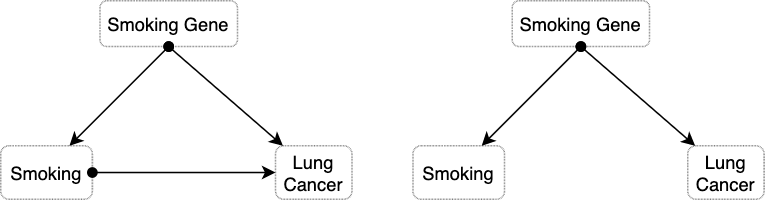
\includegraphics[width=0.7\linewidth]{Figures/SmokeDebate_diagram} 

}

\caption{The causal diagram on the left presents the situation in which the constitutional hypothesis is insufficient to explain the association between smoking and lung cancer. The diagram on the right side depicts the alternative situation in which the smoking gene fully explains the observed association.}\label{fig:smoke-debate-dia}
\end{figure}

The tobacco industry magnified any bit of controversy they could find on the scientific studies. Such organised denialism explains why the link between smoking and cancer remained so controversial in the public long after the debate was settled among epidemiologists.

\begin{quote}
Remarkably, even researchers at the tobacco companies were convinced---a fact that stayed deeply hidden until the 1990s, when litigation and whistle-blowers forced tobacco companies to release many thousands of previously secret documents. In 1953, for example, a chemist at R.J. Reynolds, Claude Teague, had written to the company's upper management that tobacco was ``an important etiologic factor in the induction of primary cancer of the lung,'' nearly a word-for-word repetition of Hill and Doll's conclusion. --- The Book of Why \citep{book-of-why}.
\end{quote}

\hypertarget{experimental-control}{%
\section{Experimental Control}\label{experimental-control}}

Experimental control entails a series of procedures for experiment and observation design aimed at minimising the effects of extraneous variables (i.e.~confounding factors) other than the manipulated variables (i.e.~independent variable) to ensure that the measured variable (i.e.~dependent variable) is only affected by the independent variables. To evaluate the effects of manipulating the independent variables, some control system is needed in which no such deliberate changes are introduced. As we have seen, sampling units (e.g.~study participants) are often divided into two groups (the experimental group and the control group) in a way that the only noticeable (or significant) difference between them lies in the stimuli exerted by the experiment.
Therefore, the control and experimental groups must be \emph{homogeneous} in all relevant factors.

In general, there are two techniques for the formation of such homogeneous groups: individual and collective control \citep{bunge2017philosophy}. \textbf{Individual control} requires simultaneous pairing of individuals in both groups, i.e.~every member of the experimental group has a corresponding equivalent member in the control group. For instance, for every thirty years old Asian man in the control group another thirty years old Asian man is assigned to the experimental group. Simultaneous pairing is complex and expensive. \textbf{Statistical control} has two main types. On one side, the \emph{control of distributions} should be performed to equate certain parameters such as averages, spreads (i.e.~std. dev.) and other collective properties (e.g.~medians). This technique is more flexible as only some properties are kept under control. In this case, we would take two samples of people with the same age and height distributions. Both simultaneous pairing and distribution control share a common disadvantage regarding the formation of the groups, which could be unintentionally biased. For instance, we could assign the strongest people to the treatment (or experimental) group to make sure they bear the treatment. To prevent this issue the two groups are usually formed at random. Thanks to \textbf{randomisation}, all variables (including most unknown factors) that were not previously controlled become randomly distributed, minimising their effect on the dependent variables. However, randomisation is not an alternative to other techniques, but rather a complement.

\hypertarget{other-experimental-control-techniques}{%
\subsection{Other experimental control techniques}\label{other-experimental-control-techniques}}

There are multiple strategies for experimental control. We have previously seen the method of division into treatment and control groups. The control and treatment groups can entail two moments in \textbf{time}, with the initial setting being the control scenario which is later on manipulated through the intervention of certain variables (e.g.~measure noise from bats in a dark chamber before and after turning a light). Another technique requires \textbf{holding certain factors constant} or finding scenarios (like in a field experiment) with the same background conditions. Nonetheless, constructing such conditions in a laboratory can also achieve this goal. In an \textbf{elimination} strategy some factors are removed to simplify study conditions, such as air resistance in a vacuum chamber or \href{https://en.wikipedia.org/wiki/Drop_tube}{drop tower}, radio waves in a Faraday cage, or gravity in space experiments. A common case of elimination is \textbf{blinding}, where subjects do not know which group they are assigned to (single blinding). Moreover, double-blinding implies hiding this information from the experimenter and/or the data analyst. Finally, we can \textbf{separate factors} by measuring their effect and correcting for it. For example, the measurements of time dilation require taking into account the Doppler effect caused by the changing distance between the observer and the moving clock. GPS systems perform adjustments due to the effects of time dilation and gravitational frequency shifts. Another example, missile trajectories are often adjusted for the effect of \href{https://en.wikipedia.org/wiki/Coriolis_force}{Coriolis force}.

\begin{center}\rule{0.5\linewidth}{0.5pt}\end{center}



\begin{figure}

{\centering 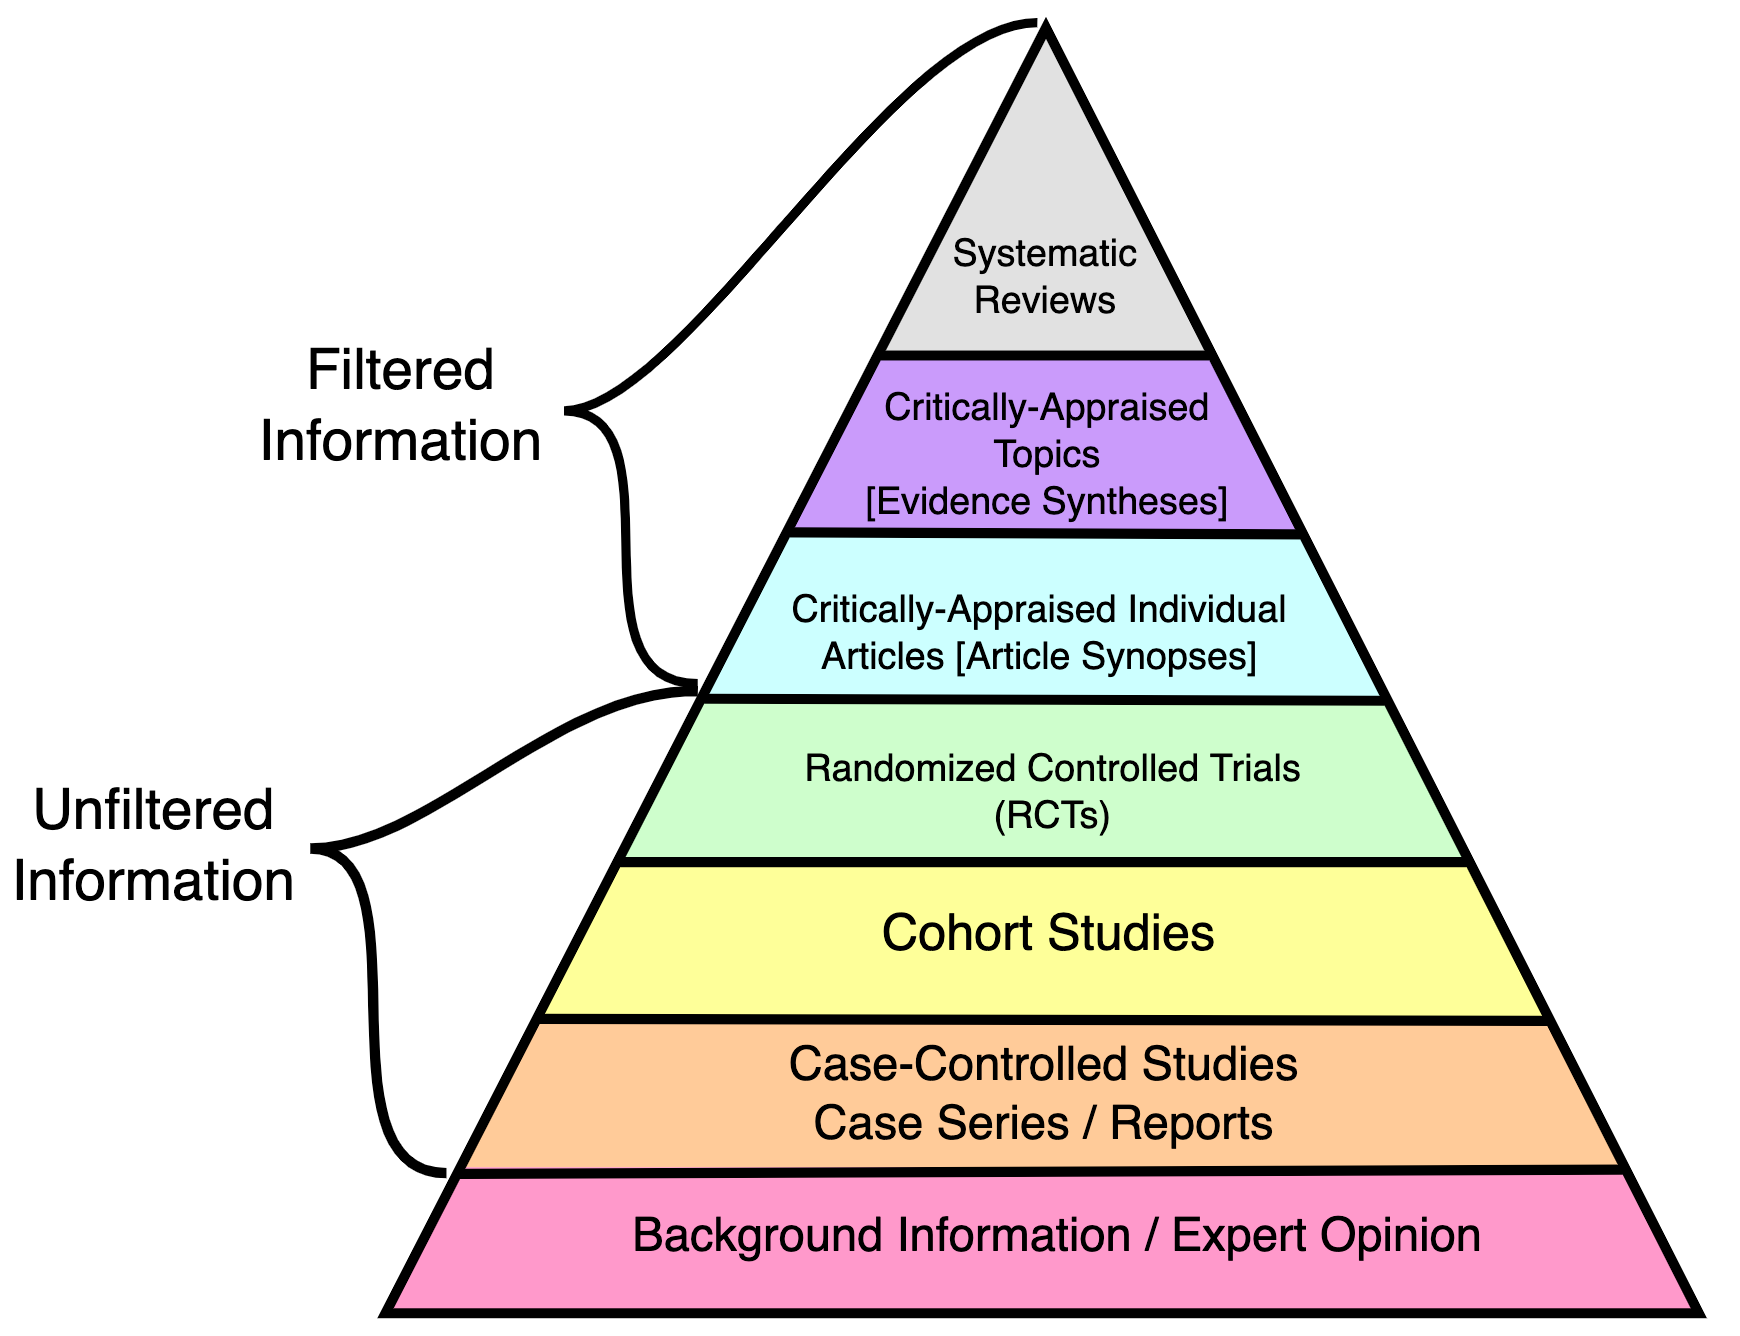
\includegraphics[width=0.7\linewidth]{Figures/pyramid-evidence} 

}

\caption{Figure from \href{https://commons.wikimedia.org/wiki/File:Research_design_and_evidence_-_Capho.svg}{Wikimedia} by CFCF. Keep in mind that this hierarchy is not free from \href{https://en.wikipedia.org/wiki/Hierarchy_of_evidence\#Criticism}{criticism} and take it just as a useful simplification.}\label{fig:pyramid-eviodence}
\end{figure}

\hypertarget{randomised-control-trials}{%
\section{Randomised Control Trials}\label{randomised-control-trials}}

The fundamental problem of causal inference tell us that it is impossible, by definition, to observe the effect of more than one treatment on a subject over a specific time period. A study participant cannot both take the pill and not take the pill at the same time. Directly observing causal effects is impossible. Nonetheless, this does not make causal inference impossible. There are certain techniques and assumptions that allow to circumvent the fundamental problem. In this context, randomized experiments allow for the estimation of population-level causal effects.

Randomisation offers a systematic solution for the division of participants (or sampling units) into two groups. In particular, RCTs are frequently regarded as a gold standard for clinical trials and among the highest quality evidence available (see Figure \ref{fig:pyramid-eviodence}). However, as with every method, it will only yield fruitful results if applied correctly, and its sole employment does not warrant against other errors.

There are different types of randomisation. In \textbf{simple randomisation}, subjects are assigned into two groups purely randomly but in small samples, we risk creating uneven groups. \textbf{Block randomisation} works by randomising participants within blocks such that an equal number are assigned to each treatment. For example, given a block size of 4, there are 6 possible ways to equally assign participants to a block (AABB, ABAB, ABBA, BAAB, BABA, BBAA). Allocation proceeds by randomly selecting one of the orderings and assigning the next block of participants to study groups according to the specified sequence. A major disadvantage of this method is that it might be possible to predict the next sequence. \textbf{Stratified randomisation} is crucial whenever all other properties (except for the factors of interest) need to be assigned equally. The study population is first stratified into subgroups (i.e.~\emph{stratas}) sharing attributes, then followed by simple or block random sampling from the subgroups.

One of the main advantages of RCTs is the reduction of selection bias or allocation bias. In Chapter \ref{stats-abuse} we will see biases in more detail. The randomisation process reduces mistrust towards a potential rigged distribution of the participants. Another common advantage is that it facilitates blinding the groups from investigators and participants.

\begin{tipbox}

\textbf{Terminology Note:}

Very often terms are used interchangeably in many domain but they can also mean different things depending on the are.

\begin{quote}
By ``allocation bias'' we understand the bias caused by allocating patients with better prognosis to either the experimental or the control group. In the context of a randomized trial the term ``selection bias'' is sometimes used instead of allocation bias to indicate selection of patients into treatment arms. We avoid the term ``selection bias'' as it has a different meaning in epidemiology more broadly: selection of non-representative persons into a study. --- \citep{paludan2016mechanisms}
\end{quote}

\end{tipbox}

However, RCTs do not necessarily ensure that background factors are equally distributed in the treatment and control groups. For small samples randomisation can provide unequal distributions. The average number after rolling a dice an infinite amount of times will converge to 3.5, but we should not be surprised if we roll a dice 10 or 20 times obtaining considerably more occurrences of the number 6 than the other numbers. The danger of relying on pure randomisation to balance covariates has been described in \citep{krause2003random} \citep{morgan2012rerandomization}. For this reason is essential to check for imbalances in known factors after randomisation. Stratified randomisation also helps balancing known factors. Nonetheless, randomisation does not necessarily guarantee full control of unknown factors but \emph{on average} their effect should be significantly smaller than the treatment applied \citep{deaton2018understanding}.

\begin{quote}
When we use an RCT to evaluate an intervention, we do so with respect to one or more endpoints (or outcomes) that will be measured in the future, after the period of intervention. It could be blood pressure, death, quality of life, etc. We want to understand the causal effect of the intervention on that outcome, but this is tricky. That's because to really understand the effect of the intervention, we would need to give it to someone and measure the outcome to see what happened. Then we would need to reset the universe back to the exact point when the intervention was given, withhold it this time, and see what happened when they were left untreated. The difference in the outcomes between the two scenarios would be our estimate of the causal effect of the intervention. This is clearly a fantasy, but hope is not lost. Thankfully we can mimic this counterfactual situation by randomizing people into groups, and since we are now talking about groups, we have to start talking about distributions of future outcomes. --- \href{https://statsepi.substack.com/p/out-of-balance}{Darren Dahly, PhD}
\end{quote}

Although RCTs are still preferred to observational studies, there are scenarios in which intervention is not possible. For instance, we cannot assign participants to be obese or not in order to study the effect of obesity on heart diseases.

\begin{wrapfigure}{R}{.25\textwidth}  
 \begin{center}
    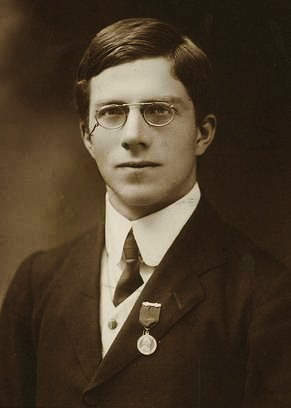
\includegraphics[width=.22\textwidth]{Figures/RAFisher.jpeg}  
  \captionsetup{labelformat=empty}
  \caption{Ronald Aylmer Fisher in 1913} 
\end{center}
\end{wrapfigure}
\addtocounter{figure}{-1}

\hypertarget{origins-of-rcts}{%
\subsection{Origins of RCTs}\label{origins-of-rcts}}

R.A. Fisher (1890-1962) conceived the RCTs in the 1930s for its employment in agriculture experiments. Fisher designed intricate approaches to disentangle the effects of fertiliser from other variables. Using the \emph{Latin Square}, he would divide the field into a grid of subplots to test each fertiliser with each combination of soil type and plant. However, in this scenario the experimenter would observe the effects of the fertiliser \emph{mixed} (i.e.~\emph{confounded}) with a variety of other things (e.g.~soil fertility, drainage, microflora). Fischer realised that the only design that would ``\emph{trick nature}'' is one where the fertilisers are assigned randomly to the subplots. Of course, sometimes you might be unlucky and assign a certain fertiliser to the least fertile subplots, but other times you might get the opposite assignment. A new random allocation is generated each time the experiment is conducted. By running the experiment multiple times the luck of each allocation is \emph{averaged}.

\begin{quote}
But Fisher realized that an uncertain answer to the right question is much better than a highly certain answer to the wrong question. {[}\ldots{]} If you ask the right question, getting an answer that is occasionally wrong is much less of a problem. You can still estimate the amount of uncertainty in your answer, because the uncertainty comes from the randomization procedure (which is known) rather than the characteristics of the soil (which are unknown). --- Section ``Why RCTs work'' in Chapter 4 from \citep{book-of-why}
\end{quote}

The Book of Why describes the aforementioned experiment in causal terms \citep{book-of-why}. The causal diagram from Figure \ref{fig:rct-diagram} depicts a model describing how the yield of each plot is determined by both the fertiliser and other variables, but the effect of the fertiliser is also affected by the same variables (red arrows). The experimenter aims to know about the effect of the fertiliser controlling for the latter effects. In other words, a model in which the effects represented by the red arrows are controlled. In this second scenario, the relation between Fertilizer and Yield is \emph{unconfounded} since there is no common cause of Fertiliser and Yield.

\begin{figure}

{\centering 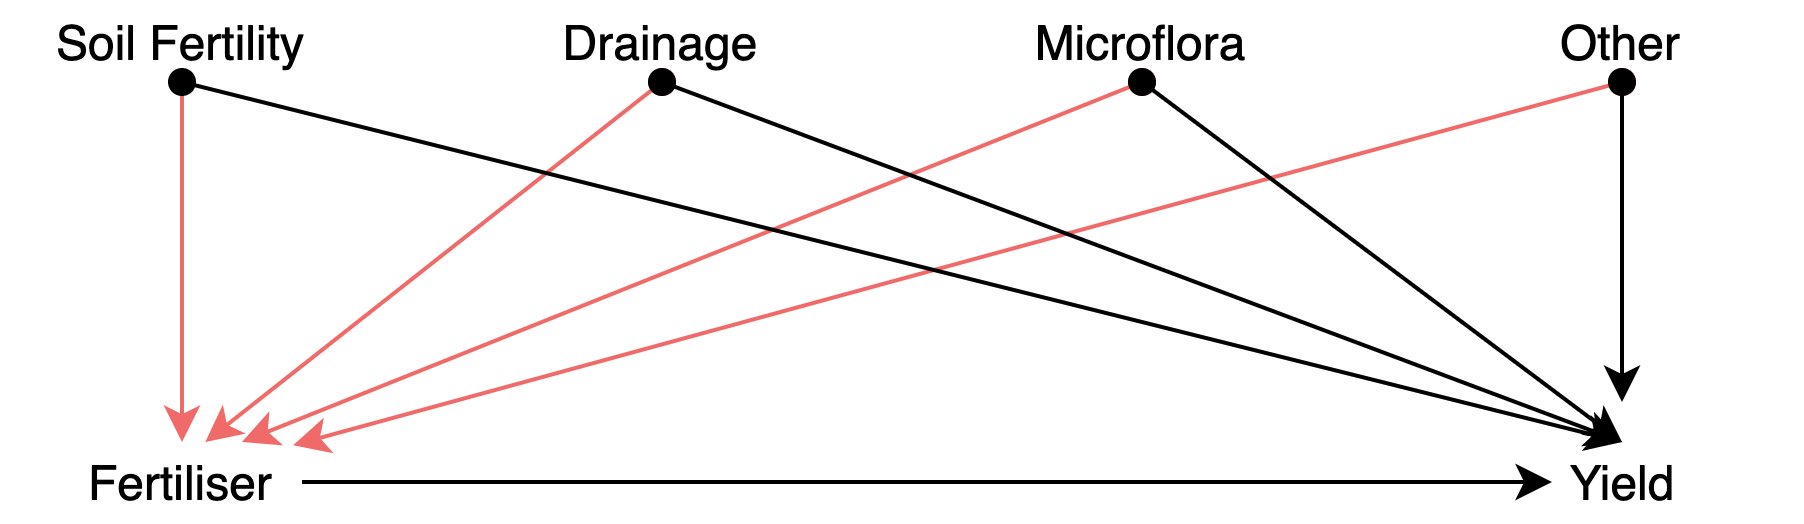
\includegraphics[width=1\linewidth]{Figures/RCT-causal-diagram} 

}

\caption{Causal diagram depicting an improperly controlled experiment.}\label{fig:rct-diagram}
\end{figure}

\hypertarget{validity}{%
\subsection{Validity}\label{validity}}

\begin{quote}
When a hypothesis is designed to explain certain observed phenomena, it will of course be so constructed that it implies their occurrence; hence, the fact to be explained will then constitute confirmatory evidence for it. But it is highly desirable for a scientific hypothesis to be confirmed also by ``new'' evidence --- by facts that were not known or not taken into account when the hypothesis was formulated. Many hypotheses and theories in natural science have indeed received support from such ``new'' phenomena, with the result that their confirmation was considerably strengthened. --- \citep{hempel-pos}
\end{quote}

Transferring RCTs results to other scenarios is not trivial. All in all, RCTs results concern a particular sample used during the study. The study sample is of course drawn from a larger group, i.e.~the population, but the RCT results cannot be simply applied to another sample drawn from the population. Randomisation is not the same as random sampling from the population. In fact, there are many RCT studies that misrepresented certain population groups. An example of women inclusion issues in clinical studies includes the under-representation of women in stroke randomized controlled trials, which leads to misleading conclusions that affect stroke care delivery \citep{tsivgoulis2017under}. A similar bias exists in animal research, including \href{https://www.wired.com/2016/07/science-huge-diversity-problem-lab-rats/}{lab mice}.

\begin{quote}
Most rodents used in biomedical studies --- the ones that suss out the effects of treatments before they make it to humans --- have boy parts and boy biological functions. And that particular kind of gender imbalance has cascading effects. A growing body of evidence indicates that females process pain differently than males. But many lab scientists who study ways of treating pain \emph{still }use all-male cohorts of lab mice. They say it's because male mice and rats aren't as hormonal as females---because isn't that what they always say---and are therefore more reliable in terms of getting data. And that means the scientific community is ignoring research that might help women manage pain better. --- \textbf{Science Has a Huge Diversity Problem\ldots{} in Lab Mice - Wired}
\end{quote}

\begin{center}\rule{0.5\linewidth}{0.5pt}\end{center}

\begin{quote}
Of 2,347 articles reviewed, 618 included animals and/or cells. For animal research, 22\% of the publications did not specify the sex of the animals. Of the reports that did specify the sex, 80\% of publications included only males, 17\% only females, and 3\% both sexes. A greater disparity existed in the number of animals studied: 16,152 (84\%) male and 3,173 (16\%) female. --- \citep{yoon2014sex}
\end{quote}

Therefore, RCTs must be internally valid, --- i.e.~the design must eliminate the possibility of bias --- but to be clinically useful the result must also be relevant to a well-defined group of patients in a particular clinical setting (i.e.~external validity). Differences between trial protocol and routine practice also affect the external validity of RCTs. In \citep{rothwell2006factors}, the authors list some of the most important potential determinants of external validity.

\hypertarget{cross-validation-in-machine-learning}{%
\section{Cross-validation in Machine Learning}\label{cross-validation-in-machine-learning}}

As data scientists, you may wonder why the previous practices are relevant to your job. In this section I want to show how similar control measures must be considered regarding machine learning (ML). When applying supervised ML methods, is important to prevent over-fitting and under-fitting situations. In particular, over-fitting occurs when a model begins to \emph{memorize} training data rather than \emph{learning} to generalize from a trend (see Figure \ref{fig:overfitting}). One of the techniques to detect or lessen the change of over-fitting includes cross-validation. The basis of this technique is to test the generalization power of the model by evaluating its performance on a set of data not used during the training stage.



\begin{figure}

{\centering 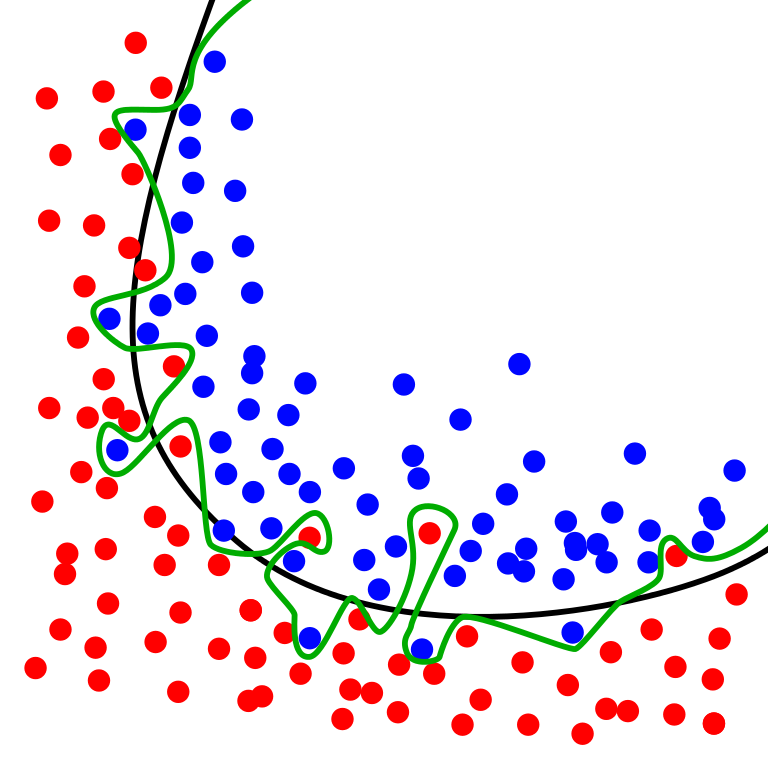
\includegraphics[width=0.45\linewidth]{Figures/Overfitting} 

}

\caption{Source: \href{https://en.wikipedia.org/wiki/File:Overfitting.svg}{Wikimedia}. The green line represents an overfitted model and the black line represents a regularized model. While the green line best follows the training data, it is too dependent on that data and it is likely to have a higher error rate on new unseen data, compared to the black line.}\label{fig:overfitting}
\end{figure}

The simplest approach is the \textbf{hold out method} which entails spliting the dataset into a train and test sets. However, yet another part of the dataset is often held out (validation set) so that the model training proceeds on the training set, the model evaluation on the validation set, and once the hyperparameters are successfully tweaked, the final evaluation is conducted on the test set. This process reduces the amount of data available for training. Cross-validation (CV) alleviates this issue.

The following procedure (see Figure \ref{fig:cross-validation}) is followed for each of the \(k\) ``folds'':

\begin{itemize}
\tightlist
\item
  A model is trained using \(k-1\) of the folds as training data.
\item
  The resulting model is validated on the remaining part of the data.
\end{itemize}

The performance measure reported by K-fold CV is then the average of the values computed in the loop. This approach can be computationally expensive, but does not waste too much data \citep{scikit-learn}.



\begin{figure}

{\centering 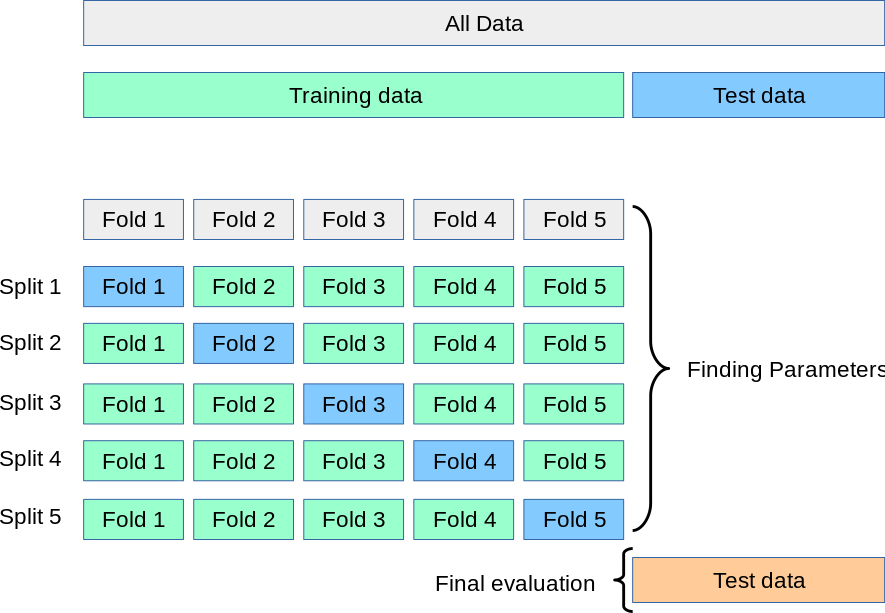
\includegraphics[width=0.75\linewidth]{Figures/grid_search_cross_validation} 

}

\caption{Source: \href{https://scikit-learn.org/stable/modules/cross_validation.html\#cross-validation}{Scikit-Learn}. A test set should still be held out for final evaluation, but the validation set is no longer needed when doing CV. In the basic approach, called K-fold CV, the training set is split into k smaller sets \citep{scikit-learn}.}\label{fig:cross-validation}
\end{figure}

However, the vanilla approach to K-fold CV does not consider certain properties of the dataset. In particular, K-fold CV is not affected by classes or groups. For instance, the training set of the first CV iteration in Figure \ref{fig:k-fold-vis} does not contain one of the classes.

\begin{figure}

{\centering 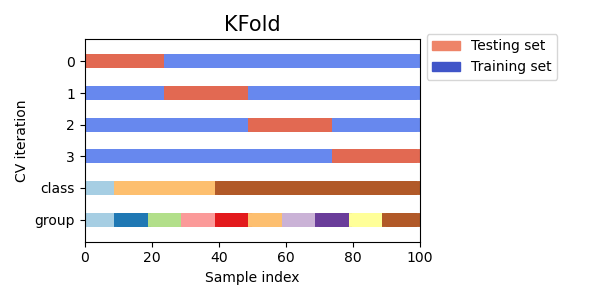
\includegraphics[width=0.63\linewidth]{Figures/k-fold-vis} 

}

\caption{Source: Scikit-Learn. K-fold CV is not affected by classes or groups.}\label{fig:k-fold-vis}
\end{figure}

Issues similar to the ones previously studied regarding RCTs can arise when conducting cross-validation. Some problems exhibit a large imbalance in the distribution of the target classes. For example, the negative class can be more representative than the positive class. In such cases, stratified sampling is recommended (see Figure \ref{fig:k-fold-strategies}) to preserve relative class frequencies in each train and validation fold.

One strong assumption of machine learning theory is that data is Independent and Identically Distributed (i.i.d.), i.e.~that all samples stem from the same generative process and that such process is assumed to have no memory regarding past samples. For example, a succession of throws of a fair coin is i.i.d. since the coin has no memory, so all the throws are independent. In this sense, if we know that the generative process has a group structure (e.g.~samples collected from different subjects, experiments, measurement devices) we should use group-wise CV. The grouping of data depends on the context. For instance, in medical data, we can find multiple samples for each patient, so it makes sense to group the samples by patient to prevent any \href{https://scikit-learn.org/0.24/common_pitfalls.html\#data-leakage}{\emph{data leakage}}. Similarly, problems where the samples have been generated using a time-dependent process call for \href{https://scikit-learn.org/stable/modules/cross_validation.html\#timeseries-cv}{time-series aware CV schemes}.



\begin{figure}

{\centering 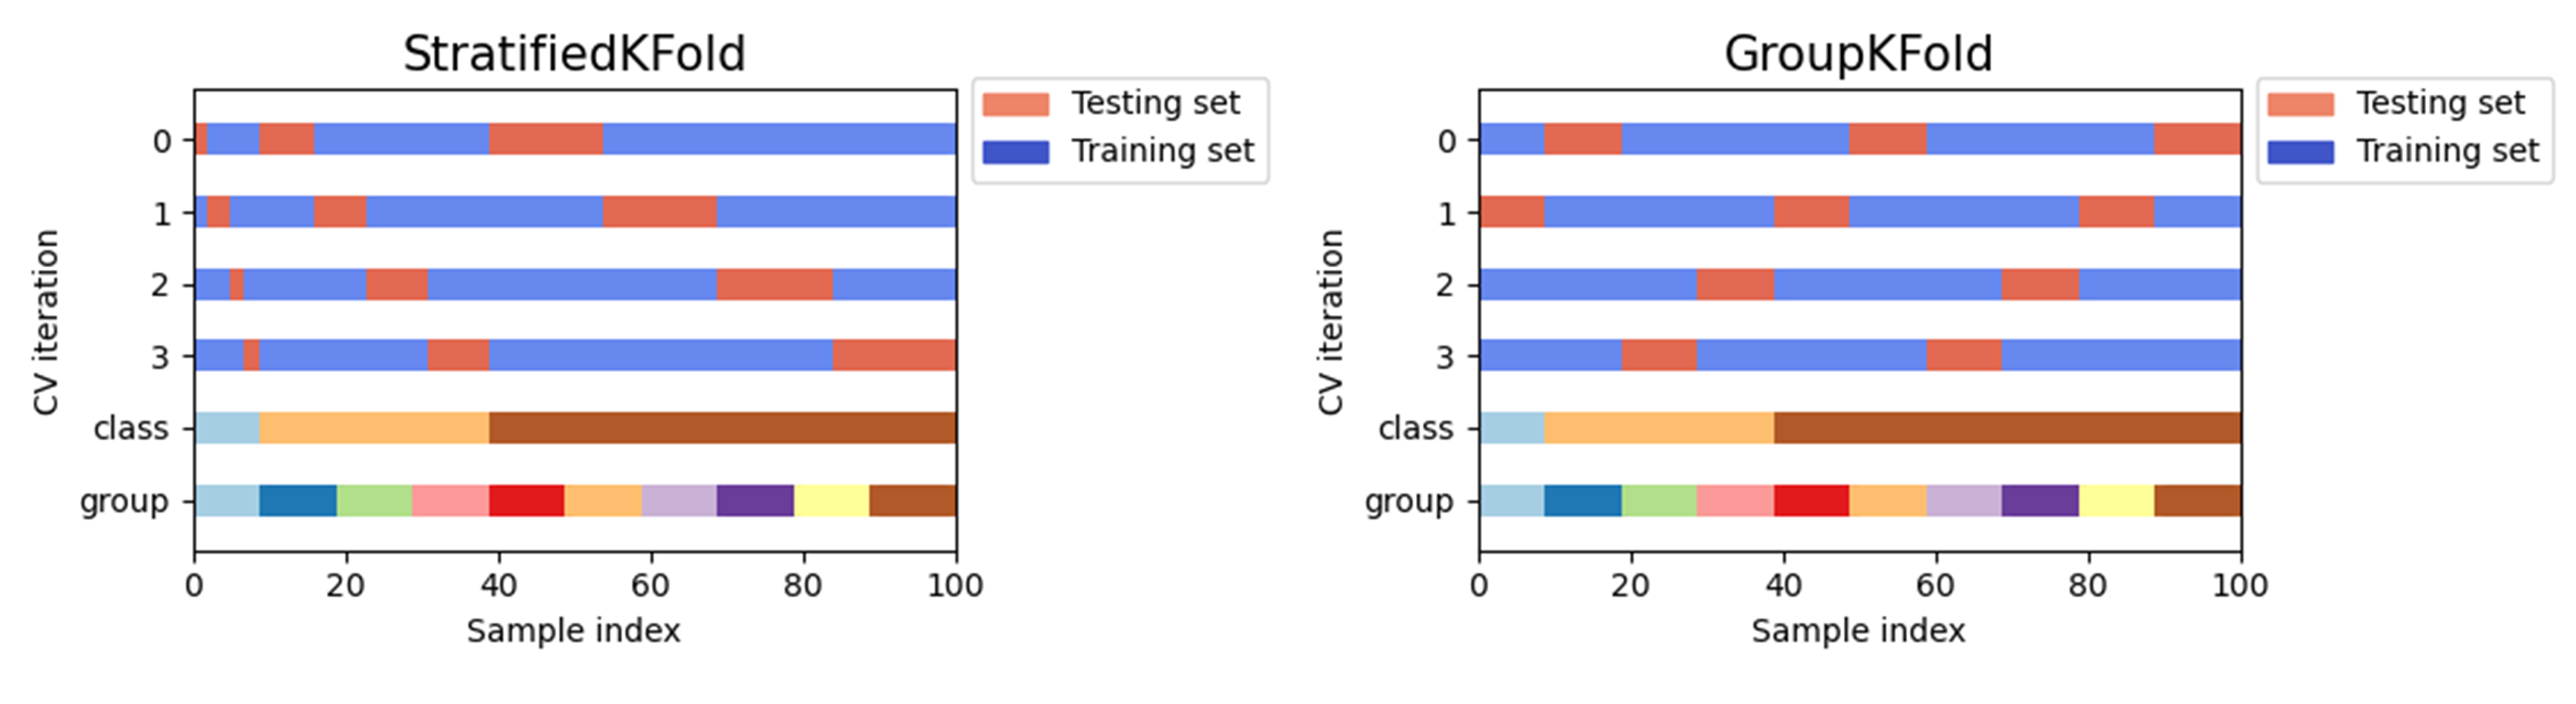
\includegraphics[width=1\linewidth]{Figures/kfold-strategies} 

}

\caption{Source: Scikit-Learn. Other K-fold CV strategies. \href{https://scikit-learn.org/stable/modules/cross_validation.html\#group-k-fold}{\textbf{GroupKFold}} is a variation of K-fold which ensures that the same group is not represented in both testing and training sets. \href{https://scikit-learn.org/stable/modules/cross_validation.html\#stratified-k-fold}{\textbf{StratifiedKFold}} is a variation of K-fold which returns stratified folds: each set contains approximately the same percentage of samples of each target class as the complete set..}\label{fig:k-fold-strategies}
\end{figure}

Similar to RTC internal validity, cross-validation does not ensure transferability to other scenarios. External validation must be performed with independent datasets to ensure robustness against new scenarios. Consider a deep-learning algorithm trained to predict the number of years a patient will survive based on its characteristics and the medication administrated. This system could be then transferred to a different hospital, in another country, region, or city where the population characteristics (diet, hygiene, professions) are different. The model will require undertaking a certain recalibration process to learn the new conditions.

\hypertarget{data-is-not-enough}{%
\section{Data alone is not enough}\label{data-is-not-enough}}

The confirmation of a hypothesis is often considered to increase as the number of favourable test findings grows, but the increase in confirmation, produced by one new favourable instance, will generally become smaller as the number of previously established favourable instances grows \citep{hempel-pos}. Many researchers and data scientists blindly rely on the dogma \emph{the more data, the merrier} but the addition of one more favourable finding raises the hypothesis confirmation but little. The confirmation of a hypothesis depends not only on the quantity of the favourable evidence available but also on its variety.

As he have seen during this course, data alone is not enough. Note that this is especially a problem for solutions based on Machine Learning, since domain knowledge or \emph{context} should be introduced somehow to \emph{direct} the model in the desired direction.

\begin{quote}
``There is no learning without bias, there is no learning without knowledge'' --- \citep{skansi2020guide} \citep{domingos2015master}.
\end{quote}

An example of how data depends on its context is user ratings or opinions. For instance, the meaning of \emph{fashionable clothes} changes over time, as do political terms. This issue is known as \emph{concept drift} \citep{kubat2017introduction}. Similarly, a text-mining engine to tag biology terms with the corresponding ontology terms may confuse elements between species, as several entities appear in multiple animals or organisms. Context is crucial for external validation and translation of solutions into real-world settings. A system for clothes recommendation should adapt to countries, cultures or ages. Similarly, a health system to predict patient risk based on disease comorbidities must be \emph{calibrated} for each country or region (e.g.~Diabetes treatment is often affordable in the EU, but an expensive treatment in the USA, which increases its mortality rate).

\begin{figure}

{\centering 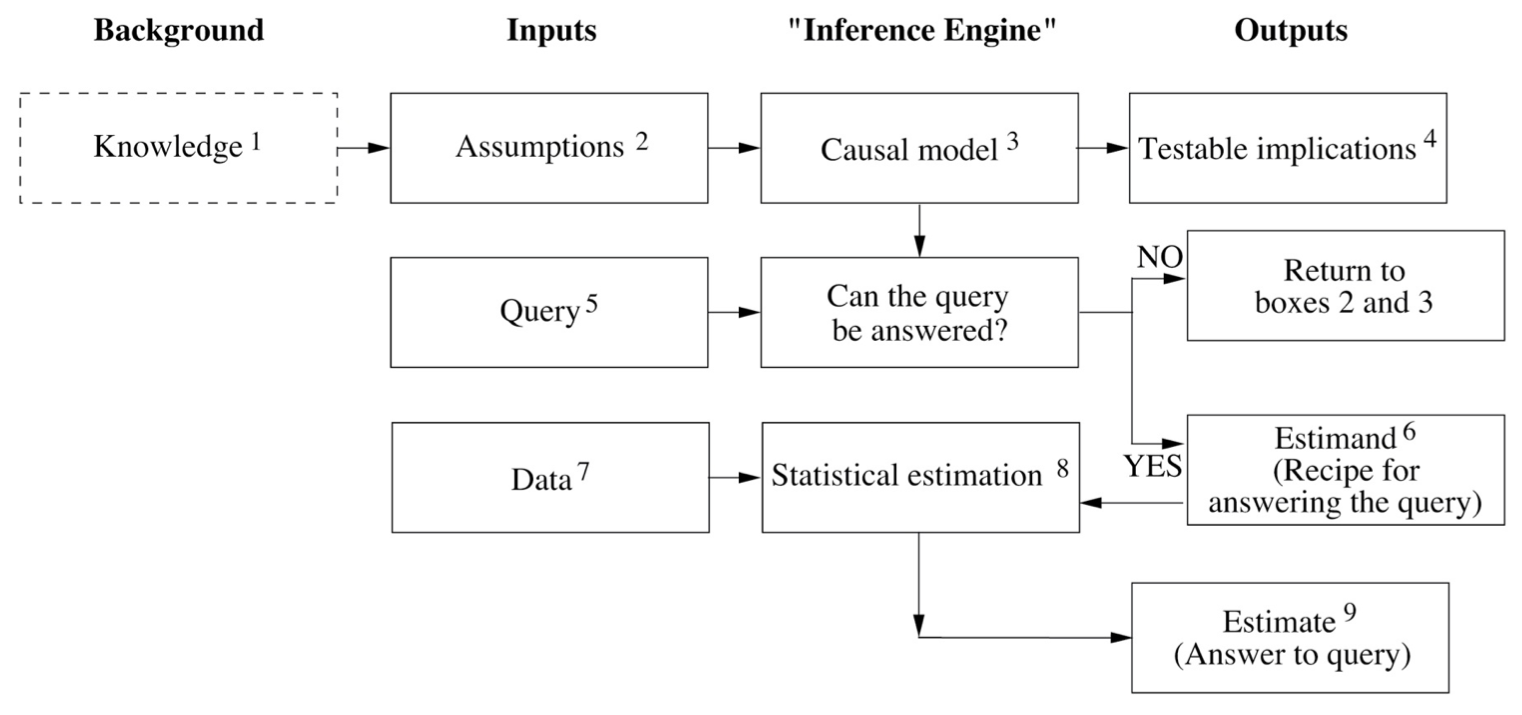
\includegraphics[width=0.9\linewidth]{Figures/jpearl_inference_engine} 

}

\caption{Diagram extracted from The Book of Why. The diagram depicts a hypothetical inference engine that combines data and causal knowledge to produce answers to questions of interest. Knowledge (dashed) is not part of the engine but required for its construction. Boxes 4 (testable implications) and 9 (estimate) could also feedback such knowledge to incrementally improve the engine.}\label{fig:inference-engine}
\end{figure}

Figure \ref{fig:inference-engine} represents an ideal causal inference engine for scientific questions. Today, causal models for scientific applications are based on a similar design. It is important to notice how this diagram showcases the importance of extra-observational information (i.e.~information other than data) such as \textbf{assumptions}, which derive from the available \textbf{knowledge}. With them, a \textbf{causal model} is built in any of its different forms, e.g.~logical statements, structural equations, causal diagrams, etc. Causation (or a causation assumption) can be defined from the following analogy, \(X\) is a cause of \(Y\) if \(Y\) \emph{listens} to \(X\) and determines its value in response to what it hears. For instance, the patient's lifespan \(L\) is determined by the intake of drug \(D\). In this case, \(D\) acts as a cause of \(L\) (although it might not be the only cause), which is represented by an arrow from \(D\) to \(L\) in a causal diagram (see Figure \ref{fig:blueprint}). For the sake of simplicity the other causes of \(L\) can be grouped in an additional variable \(Z\).

In box \(4\) the patterns encoded in the paths of the causal model yield a series of observable consequences (or data dependencies), that we know as \textbf{testable implications} (remember the hypothetico-deductive method?). These implications can be used to test the model. For instance, the lack of path between \(D\) and \(L\) would imply that \(D\) and \(L\) are independent, meaning that a variation of \(D\) will not alter \(L\). If such implication is contradicted by the data, the model should be revised bearing in mind this new knowledge. The box \(5\) is in charge of the scientific \textbf{query} which must be encoded in causal vocabulary, e.g.~\(P(L | do(D))\), i.e.~what is the probability that a typical patient would live \(L\) years given that it takes the drug \(D\)?.

\begin{figure}

{\centering 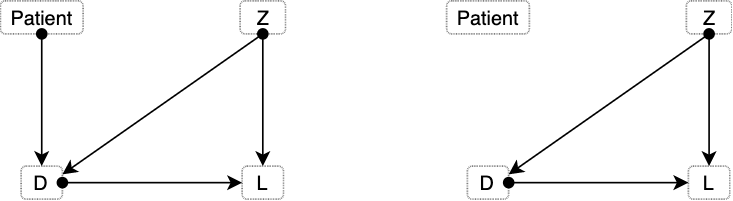
\includegraphics[width=0.7\linewidth]{Figures/blueprint} 

}

\caption{Diagram depicting two different scenarios: before, and after an intervention.}\label{fig:blueprint}
\end{figure}

The \(do()\) operator represents an intervention in the system, in contrast to an observation \(P(L|D)\). An instance of the latter would entail letting the patient decide between taking or not the drug (see left side of Figure \ref{fig:blueprint}). Such decision might be affected by other variables we are not aware, like the patient's education, family, etc. However, when we make an intervention and assume that we are giving the drug to the patient, the arrow illustrating the patient's decision disappears (right side of Figure \ref{fig:blueprint}).

The \textbf{\emph{estimand}} is the recipe to answer the scientific query, written as a probability formula, such as \(P(L | D, Z) \times P(Z)\). Once the \textbf{data} is introduced, an \textbf{estimate} can be calculated. Importantly, some queries may not be answerable regardless of the amount of data collected. For instance, our causal model could indicate that both \(D\) and \(L\) depend upon a third variable \(Z\). If there would not be any way to measure \(Z\), the query \(P(L | do(D))\) would be unanswerable. Collecting data for this question would be worthless. Under such a scenario, the causal model needs to be reviewed. Either to introduce new knowledge to enable estimating \(Z\), or to simplify the previous assumptions, potentially increasing the risk of wrong answers, e.g.~stating that \(Z\) has a negligible effect on \(D\).

Following the analogy, the data acts as the ingredients of the recipe provided by the \emph{estimand}. Our estimate (box \(9\)) represents an approximate answer to the query. Such an answer is approximate because data always represents a finite sample from a theoretically infinite population \citep{book-of-why}. An example of answer in this case could be that drug \(D\) increases lifespan \(L\) of diabetic patients by \(30\% \pm 10\%\).

The most important fact about the diagram in Figure \ref{fig:inference-engine} is that data and causal model are two independent pieces of the puzzle that later work together. Data is collected after the causal model and stating that the scientific query can be answered. The \emph{estimand} computation does not require any data. Comparing this to conventional machine learning (ML) systems, an ML solution would have to be re-trained when moved from one hospital to another since such model just fitted a function to data, without levering from any causal model.

\hypertarget{examples-3}{%
\section{Examples}\label{examples-3}}

\hypertarget{covid-israel}{%
\subsection{Covid-19: How can efficacy versus severe disease be strong when 60\% of hospitalized are vaccinated?}\label{covid-israel}}

\begin{rnote}
\emph{There are three kinds of lies: Lies, damned lies, and statistics}

\end{rnote}

In this \href{https://www.covid-datascience.com/post/israeli-data-how-can-efficacy-vs-severe-disease-be-strong-when-60-of-hospitalized-are-vaccinated}{blog post}, biostatistics Professor Jeffrey Morris demonstrates how without properly controlling for age, efficacy against severe disease in Israel may appear weak when in fact within each age-group it is extremely strong. Consider the table from Figure \ref{fig:vaccine-rates-a} and the following data from the the Israeli government. As of August 15, 2021 nearly 60\% of all patients currently hospitalized for COVID-19 are vaccinated. Out of 515 patients currently hospitalized with severe cases in Israel, 301 (58.4\%) of these cases were fully vaccinated.

\begin{figure}

{\centering 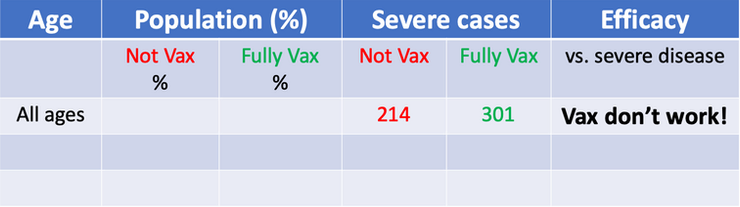
\includegraphics[width=0.7\linewidth]{Figures/vaccines-ex-fig1} 

}

\caption{Misleading table. This kind of tables have been used to claim that vaccines do not work or that its efectiveness reduces over time.}\label{fig:vaccine-rates-a}
\end{figure}

The numbers are true, but we need more than that to draw a proper conclusion about vaccine efficacy. Consider the following extreme scenarios. If the number of vaccinated people would be 0 we would expect all severe cases to be not vaccinated (obviously). On the other hand, if 100\% of people would have been vaccinated, we would expect all severe cases to proceed from vaccinated people and 0 from non vaccinated. In this case, we have an in-between situation where 80\% of residents (older than 12 years) have been vaccinated. Therefore, since the group of vaccinated people is larger than the non-vaccinated, we can expect more severe cases in absolute numbers. However, once we adjust for vaccination rates and normalise the counts, the story changes. The rate of severe cases is three times higher in unvaccinated individuals.

\begin{figure}

{\centering 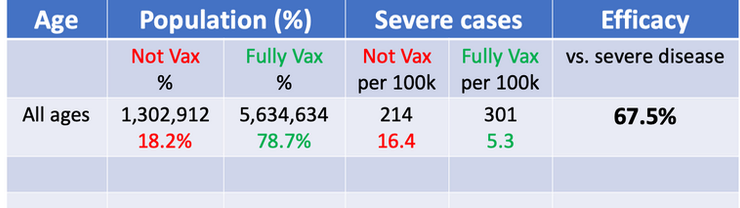
\includegraphics[width=0.7\linewidth]{Figures/vaccines-ex-fig2} 

}

\caption{Table adjusted for vaccination rates.}\label{fig:vaccine-rates-b}
\end{figure}

\begin{quote}
Vaccine Efficacy vs.~Severe disease = 1 - 5.3/16.4 = 67.5\%.
The interpretation of this number is that the vaccines are preventing \textgreater2/3 of the serious infections leading to hospitalization that would have occurred sans vaccination.
\end{quote}

Still, the obtained efficacy is lower than what we would expect. There are other factors that contribute to this confusion, including: age disparity in vaccinations, old people is more likely to be hospitalized than young people, etc.

I recommend going through the blog post to see how the author continues to apply adjustments and stratifications to find the true efficacy of the vaccines. Moreover, this is a good example of the Simpson's paradox, where misleading results can be obtained in the presence of confounding factors.

\begin{quote}
In conclusion, as long as there is a major age disparity in vaccination rates, with older individuals being more highly vaccinated, then the fact that older people have an inherently higher risk of hospitalization when infected with a respiratory virus means that it is always important to stratify results by age; Even more fundamentally, it is important to use infection and disease rates (per 100k, e.g.) and not raw counts to compare unvaccinated and vaccinated groups to adjust for the proportion vaccinated. Use of raw counts exaggerates the vaccine efficacy when vaccinated proportion is low and attenuates the vaccine efficacy when, like in Israel, vaccines proportions are high.
\end{quote}

\hypertarget{viz-hurricane}{%
\subsection{Misinterpretations of hurricane forecast maps}\label{viz-hurricane}}

The \href{https://www.nytimes.com/interactive/2019/08/29/opinion/hurricane-dorian-forecast-map.html}{following article} by Alberto Cairo published in The New York Times explains how hurricane cone forecast maps can mislead the public and produce real-world consequences.

\begin{figure}

{\centering 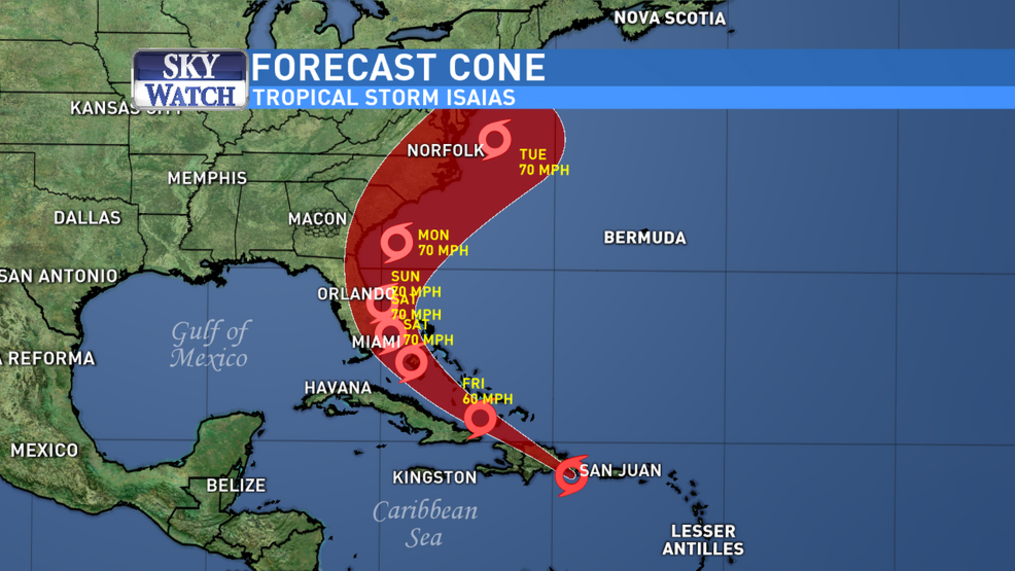
\includegraphics[width=0.66\linewidth]{Figures/hurricane-forecast-maps-tv} 

}

\caption{Example of hurricane forecast cone graphic in TV.}\label{fig:hurricane-tv}
\end{figure}

\href{https://www.semanticscholar.org/paper/Misinterpretations-of-the-\%E2\%80\%9CCone-of-Uncertainty\%E2\%80\%9D-in-Broad-Leiserowitz/f7c04b6eb883cf7d7fdee007cda056ed18182829}{Studies} show that people can misinterpret this type of map as indicating that the hurricane will get bigger over time. Others think it shows areas under threat. Recent \href{https://interactive.miami.edu/hurakan/}{research} suggests that 40\% of people would not feel threatened if they lived just outside of the cone. Moreover, people who live inside the cone, but far from the center, take less precautions than those closer to the central line. These misunderstandings have real-world consequences. Actually, the cone represents a range of possible positions and paths for the storm's center. The dots in the middle of the cone correspond to the forecast of where the hurricane's center could be in the following five days. But there's a good chance that the actual center of the storm will not end up being at those positions.

To create the cone, the National Hurricane Center (N.H.C.) surrounds each estimated position of the storm center with circles of increasing size. \textbf{These circles represent uncertainty}, meaning that the storm center may end up being anywhere inside the circles --- or even outside of them. The uncertainty circles grow over time because it is more difficult to to predict what will happen in five days from now than in one day. Finally, a curve connects the circles, resulting in what is popularly known as the `cone of uncertainty'.

\begin{figure}

{\centering \includegraphics[width=0.66\linewidth]{Figures/hurricane-forecast-maps} 

}

\caption{Cone of uncertainty.}\label{fig:hurricane-map}
\end{figure}

\begin{quote}
N.H.C. says cones will contain the path of the storm center only 60 to 70 \% of the time. In other words, one out of three times we experience a storm like this, its center will be outside the boundaries of the cone. Hurricanes are also hundreds of miles wide, and the cone shows only the possible path of the storm's center. Heavy rain, storm surges, flooding, wind and other hazards may affect areas outside the cone. The cone, when presented on its own, doesn't give us much information about a hurricane's dangers. The N.H.C. designs other graphics, including this one showing areas that may be affected by strong winds. But these don't receive nearly as much attention as the cone. The cone graphic is deceptively simple. That becomes a liability if people believe they're out of harm's way when they aren't. As with many charts, it's risky to assume we can interpret a hurricane map correctly with just a glance. Graphics like these need to be read closely and carefully. Only then can we grasp what they're really saying.
\end{quote}

\begin{rnote}
From a \href{https://www.nytimes.com/interactive/2019/08/29/opinion/hurricane-dorian-forecast-map.html}{NYT article} by Alberto Cairo

\end{rnote}

\begin{figure}

{\centering \includegraphics[width=0.66\linewidth]{Figures/hurricane-forecast-heat-map} 

}

\caption{Other graphics designed by USA National Hurricane Center.}\label{fig:hurricane-heatmap}
\end{figure}

\hypertarget{ethics-and-responsibility}{%
\chapter{Ethics and Responsibility}\label{ethics-and-responsibility}}

\begin{notebox}

\begin{center}
\textbf{Course Note:}

\end{center}

This chapter is under construction. Content is hidden.

\end{notebox}

\hypertarget{wont-fix}{%
\chapter{Extra Material}\label{wont-fix}}

This section includes related questions and topics not tackled in this course.

\hypertarget{history-of-science}{%
\section{History of science}\label{history-of-science}}

Although many historical examples are given to the students to illustrate the different chapters and topics addressed in this course, the history of science is not part of the course curriculum. However, we aim to include a rich but brief summary of the history of science as optional reading in further semesters of this course.

\hypertarget{theory-relatedness-of-observations}{%
\section{Theory-relatedness of observations}\label{theory-relatedness-of-observations}}

In the philosophy of science, observations are said to be ``theory-laden'' when they are affected by the theoretical presuppositions held by the investigator. This thesis of theory-ladenness is associated with the works of Thomas Kuhn and perhaps first put forth by Pierre Duheem \citep{sep-science-theory-observation}.

\begin{quote}
``A related topic is the theory-relatedness of observations; some have claimed that there are no such things as fully theory-independent observations. If true, it would undermine the possibility of objectivity of science and force us to accept strong relativism. I believe that this disastrous consequence can be avoided and that there really is a basis of theory-neutral data, also in the humanities.'' -- {[}johansson2016philosophy{]}.
\end{quote}

\begin{quote}
The question then arises: is it just as easy to distinguish between theoretical statements and observational statements? The answer is no, as can be seen from the previous examples regarding how unconscious background beliefs can affect what is observed and reported even a in a very simple tasks such as time measurements. -- {[}johansson2016philosophy{]}.
\end{quote}

\hypertarget{gettier-problems}{%
\section{Gettier problems}\label{gettier-problems}}

The definition of knowledge is an ongoing debate among epistemologists. Although the three criteria from Plato are necessary conditions, they are not sufficient as there are situations that satisfy all these conditions and yet don't constitute knowledge (see \href{https://en.wikipedia.org/wiki/Gettier_case}{Gettier cases}) but such cases are rather philosophical and will not be discussed during this course.

\hypertarget{realism}{%
\section{Realism and anti-realism}\label{realism}}

For now this will not be included as part of the course curriculum. For a short account of this topic, read Chapter 4 from \citep{okasha-pos}.

  \bibliography{book.bib,packages.bib}

\end{document}
